\documentclass[12pt]{article}

\usepackage{graphics}
\usepackage{epsfig,dsfont}
\usepackage{times,tikz, tikz-qtree}
\usepackage{amsmath, amssymb, hyperref,float}
\usepackage[nottoc,numbib]{tocbibind}
\usepackage{framed, pseudocode}
\usepackage{mathrsfs} 
\usepackage{graphicx, dsfont}
\usepackage{amsthm,fullpage}
\usepackage{graphicx,float,hyperref}
\usepackage{verbatim}
\usepackage{multirow} % for column and two spanning in tables
\usepackage{subfigure}
\usepackage[ruled,vlined]{algorithm2e}

%%%%----------------------------------------- Code for notation list
% Macro for 'List of Symbols', 'List of Notations' etc...
\def\listofsymbols{ 
 
 %%% this file lists the notations used in the thesis for the reader's benefit and for clarity of exposition. 
 
 % to define a new symbol use the command:   \newnot{symbol:nml} for example.  
 
 
 %%%%%%%%%%%%%%%%%%%%%%%
%Sample List of Symbols
%%%%%%%%%%%%%%%%%%%%%%%
{\Huge\textbf{List of Symbols}}
\begin{tabbing}
% YOU NEED TO ADD THE FIRST ONE MANUALLY TO ADJUST THE TABBING AND SPACES
%$\vert \vec{x} \vert_{\nu} = \left(\sum_{i=1}^d\vert x_i\vert^\nu\right)^{1/\nu}$~~~~~\=\parbox{4.5in}{The $\nu$ norm of the vector $\vec{x}$.\dotfill \pageref{symbol:norm}}\\
$ \vec{a}$~~~~~~~~~~~~~~~~~~~~~~~~~~~~~~~~~~~~~~~~\=\parbox{4.5in}{A column vector of entries $a_i$ for $i=1,\dots,d$. \dotfill \pageref{symbol:vec} }\\

%ADD THE REST OF SYMBOLS WITH THE HELP OF MACRO
%\addsymbol : {}{symbol:proptp}
%\addsymbol \vert \vec{x} \vert_{\nu} = \left(\sum_{i=1}^d\vert x_i\vert^\nu\right)^{1/\nu}: {\hspace{1.2in}The $\nu$ norm if the vector $\vec{x}$.}{symbol:norm}
%\addsymbol \vec{a}: {A column vector of entries $a_i$ for $i=1,\dots,d$.}{symbol:vec}
$\vert \vec{x} \vert_{\nu} = \left(\sum_{i=1}^d\vert x_i\vert^\nu\right)^{1/\nu}$~~~~~\=\parbox{4.5in}{The $\nu$ norm of the vector $\vec{x}$.\dotfill \pageref{symbol:norm}}\\
\addsymbol \mathds{1}[A]: {Indicator function for the set $A$.}{symbol:ind_A}
\addsymbol N_{[a,b]}(A\vert B,C): {\hspace{.0in}Normal density on $A$, with mean $B$, and variance $C$, truncated to $[a,b]$.}{symbol:normal}
\addsymbol \sim: {Distributed as, or, Distributed according to the density.}{symbol:sim}
\addsymbol \propto: {Proportional to}{symbol:propto}
\addsymbol R(\mathcal{T}_i): {\hspace{.0in}The risk of the $i$th tree.}{symbol:risk_tree}
\addsymbol \text{Inv\textendash Gamma}(A\vert B,C): {\hspace{.0in}Inverse gamma density on $A$, with shape $B$, and scale $C$. }{symbol:inv_gamma}
\addsymbol \text{Multinomial}(A\vert B, C): {\hspace{.0in}Multinomial mass function on A, with count $B$ and probabilities $C$.}{symbol:mult}
\addsymbol \text{Dirichlet}(A\vert B): {\hspace{.0in}Dirichlet density on $A$ with concentration parameters $B$.}{symbol:dirichlet}
\addsymbol s(\mathcal{A},n): {\hspace{.0in}The shatter coefficient for sets $\mathcal{A}$ on sample size $n$.}{symbol:shatter_coef}
\addsymbol V_\mathcal{A}: {\hspace{.0in}The VC dimension for functions in the class $\mathcal{A}$. }{symbol:VC_dim}
\addsymbol v_n=\frac{\sum_{i=1}^n\mathds{1}(y_i =\hat{\mathcal{T}}(X_i))}{n}: {\hspace{.0in}The empirical error of the classifier.}{symbol:empirical_error}
\addsymbol v=\Pr(\mathcal{T}(X)=y): {\hspace{.0in}The theoretical (Bayes) error of the classifier.}{symbol:true_error}
\addsymbol \mathcal{H}(x): {\hspace{.0in}The entropy function.}{symbol:entropy}
\addsymbol \mathbb{R}: {\hspace{.0in}The real number system.}{symbol:real}
\addsymbol \mathbb{S}^d: {\hspace{.0in}The $d$-dimensional simplex.}{symbol:simp}
\addsymbol J(\vec{y}\vert\vec{x}): {\hspace{.0in}The Jacobian of the transformation from $\vec{y}$ to $\vec{x}$.}{symbol:jacobian}
\addsymbol Diag(a_i): {\hspace{.0in}A square, diagonal matrix with diagonal entries $a_i$.}{symbol:diag}
\addsymbol \mathcal{O}(A): {\hspace{.0in}Big ``O'' of $A$.}{symbol:big_oh}
\addsymbol \odot: {\hspace{.0in}Hadamard product of two vectors (element-wise product).}{symbol:hadamard}
\addsymbol MVN(\vec{a} \vert \vec{b}, C): {\hspace{.0in}Multivariate normal on $\vec{a}$, with mean $\vec{b}$, and covariance $C$.}{symbol:mvn}
\addsymbol S\beta(c\vert \alpha, \beta, a, b): {\hspace{.0in}Scaled beta distribution on $c$ with parameters $\alpha$, $\beta$, scaled to the support $[a,b]$. }{symbol:scaled_beta}
\addsymbol \Phi,\ \ (\Phi^{-1}): {\hspace{.0in}Cumulative density  (quantile) function for the standard normal.}{symbol:sncdf}
\addsymbol Unif(A,B): {\hspace{.0in}Continuous uniform density on the region $[A,B]$.}{symbol:unif}
\addsymbol \text{Exponential}(\lambda): {\hspace{.0in}The exponential density with rate $\lambda$.}{symbol:exponential_dist}
\addsymbol \text{Laplace}(\mu,\sigma): {\hspace{.0in}Laplace density with location $\mu$ and scale $\sigma$. }{symbol:laplace_dist}
%\addsymbol \text{Inv-Wishart}(A \vert B,C): {\hspace{.0in}Inverse Wishart distribution on $A$, with degrees of freedom $B$ and matrix $C$}{symbol:inv_wishart}
%\addsymbol \text{tr}(A): {\hspace{.0in}The trace of the matrix A, the sum of the diagonal elements.}{symbol:trace}

% .
% .
% .
% .
% ALWAYS KEEP THE FOLLOWING LINE
\end{tabbing} \clearpage}
\def\addsymbol #1: #2#3{$#1$ \> \parbox{4.5in}{#2 \dotfill \pageref{#3}}\\} 
\def\newnot#1{\label{#1}} 
%%%%%--------------------------------------End of code for notation list


%%%%----------------------------------------- Code for abbreviation list
% Macro for 'abbreviations' etc...
\def\listofabbreviations{ 
 
 %%% this file lists the notations used in the thesis for the reader's benefit and for clarity of exposition. 
 
 % to define a new symbol use the command:   \newabbrev{abbrev:nml} for example.  
 
 
 %%%%%%%%%%%%%%%%%%%%%%%
%Sample List of Abbrevations
%%%%%%%%%%%%%%%%%%%%%%%
{\Huge\textbf{List of Abbreviations}}
\begin{tabbing}
% YOU NEED TO ADD THE FIRST ONE MANUALLY TO ADJUST THE TABBING AND SPACES
CS~~~~~\=\parbox{6in}{\hspace{.4in}Computer science\dotfill \pageref{abbrev:CS}}\\
%ADD THE REST OF SYMBOLS WITH THE HELP OF MACRO
%\addsymbol : {}{symbol:proptp}
\addabbrev GLM : {\hspace{.4in}Generalized linear model}{abbrev:GLM}
\addabbrev GLMM : {\hspace{.4in}Generalized linear mixed model}{abbrev:GLMM}
\addabbrev UCI: {\hspace{.4in}University of California Irvine}{abbrev:UCI}
\addabbrev ALN: {\hspace{.4in}Additive logistic regression}{abbrev:ALN}
\addabbrev CART: {\hspace{.4in}Classification and Regression Tree}{abbrev:CART}
\addabbrev CGM: {\hspace{.4in}Chipman, George and McCulloch}{abbrev:CGM}
\addabbrev DMS: {\hspace{.4in}Denison, Mallick and Smith}{abbrev:DMS}
\addabbrev MH: {\hspace{.4in}Metropolis-Hastings}{abbrev:MH}
\addabbrev MCMC: {\hspace{.4in}Markov chain Monte Carlo}{abbrev:MCMC}
\addabbrev FS: {\hspace{.4in}Forward selection}{abbrev:FS}
\addabbrev SSVS: {\hspace{.4in}Stochastic search variable selection}{abbrev:SSVS}
\addabbrev RJ-MCMC: {\hspace{.4in}Reversible jump Markov chain Monte Carlo}{abbrev:RJ-MCMC}
\addabbrev LAR: {\hspace{.4in}Least angle regression}{abbrev:LAR}
\addabbrev LASSO: {\hspace{.4in}Least absolute shrinkage and selection operator}{abbrev:LASSO}
\addabbrev UUP: {\hspace{.4in}Uniform uncertainty principle}{abbrev:UUP}
\addabbrev MSE: {\hspace{.4in}Mean squared error}{abbrev:MSE}
\addabbrev VIMP: {\hspace{.4in}Variable importance}{abbrev:VIMP}
\addabbrev ZIP: {\hspace{.4in}Zero-inflated Poisson}{abbrev:ZIP}
\addabbrev GP: {\hspace{.4in}Gaussian process}{abbrev:GP}
\addabbrev VC: {\hspace{.4in}Vapnik-Chervonenkis}{abbrev:VC}
\addabbrev DGP: {\hspace{.4in}Data generating process}{abbrev:DGP}
\addabbrev MVN: {\hspace{.4in}Multivariate normal}{abbrev:MVN}
\addabbrev ZINB: {\hspace{.4in}Zero-inflated negative binomial}{abbrev:ZINB}
\addabbrev DiVaS: {\hspace{.4in}Dirichlet variable selection}{abbrev:DiVaS}
\addabbrev ALoVaS: {\hspace{.4in}Additive logistic variable selection}{abbrev:ALoVaS}
\addabbrev ALT: {\hspace{.4in}Additive logistic transformation}{abbrev:ALT}
\addabbrev GL: {\hspace{.4in}Gramacy and Lee}{abbrev:GL}
\addabbrev DGP: {\hspace{.4in}Data generating process}{abbrev:DGP}
\addabbrev MTD: {\hspace{.4in}Markov transition density}{abbrev:MTD}
\addabbrev CHAID: {\hspace{.4in}Chi-squared automatic interaction detection}{abbrev:CHAID}
\addabbrev GIG: {\hspace{.4in}Generalized inverse Gaussian}{abbrev:GIG}
\addabbrev MGF: {\hspace{.4in}Generalized inverse Gaussian}{abbrev:MGF}



% ALWAYS KEEP THE FOLLOWING LINE
\end{tabbing} \clearpage}
\def\addabbrev #1: #2#3{#1 \> \parbox{6in}{#2 \dotfill \pageref{#3}}\\} \def\newabbrev#1{\label{#1}} 
%%%%%--------------------------------------End of code for notation list


\newtheorem{mydef}{Definition}
\newtheorem{lem}{Lemma}
\newtheorem{thrm}{Theorem}

\graphicspath{ {/Users/rlucas7/Dropbox/Public/Thesis_Proposal/figures/} }
%\graphicspath{ {images_folder/}{other_folder/}{third_folder/} } use this if there are several filepaths or folders for images 

%for fancy script letters... $\mathscr{ABCDEFGHIJKLMNOPQRSTUVWXYZ}$
\newcommand{\Risk}{(1/n)\sum_{i=1}^n\mathbb{I}(g(Z_i)=y_i)}
\newcommand{\erisk}{(1/n)\sum_{i=1}^n\mathbb{I}(\hat{g}(Z_i)=y_i)}
\newcommand{\bayesorprob}{Bayesian}
\newcommand{\yvec}{\underline{y}}
\newcommand{\xvec}[0]{\underline{x}}
\newcommand{\simp}[1]{\mathbb{S}^{#1}}
\newcommand{\Rsp}[1]{\mathbb{R}^{#1}}
\newcommand{\muvec}[0]{\underline{\mu}}
\renewcommand{\vec}[1]{\underline{{#1}}}
\newcommand{\iid}[0]{$i.i.d.$}
\newcommand{\invgam}[3]{\text{Inv-Gamma}({#1}\vert{#2},{#3})}
\newcommand{\Sbeta}[4]{S\beta(#1\vert#2, #3, #4)}
\newcommand{\ALT}{ALT}
\newcommand{\ALN}{ALN}
%\usepackage[mathscr]{euscript} 
% for less fancy script letters... $\mathscr{ABCDEFGHIJKLMNOPQRSTUVWXYZ}$

% The proposal format is the following:
%        30 pages
%        12 point type
%        1 inch margins all around = 6.5   inch columnT
%        (Total:  30 * 6.5   = 195 page-inches)
%
% For letter-size paper: 8.5 in x 11 in
% Latex Origin is 1''/1'', so measurements are relative to this.

\linespread{1.7} % 1.6 = double space, 1.3 = 1.5 space comment out for regular


\topmargin      0.0in
\headheight     0.0in
\headsep        0.0in
\oddsidemargin  0.0in
\evensidemargin 0.0in
\textheight     9.0in
\textwidth      6.5in


\title{{\bf Doctoral Thesis } \\
\it Submitted to the faculty at Virginia Tech}
\author{ {\bf Lucas Roberts}  \\
Department of Statistics \\
Virginia Tech \\
{\small rlucas7@vt.edu}
}
\date{\today}




\begin{document}
\pagestyle{plain}
\pagenumbering{roman}
\maketitle


\pagebreak
\begin{abstract}
In this thesis we provide a historical survey of the statistics and computer science research in decision trees. We review both the greedy and Bayesian approaches to decision tree induction and propose a novel modification to previous Bayesian decision tree methods. Our approach facilitates covariate selection explicitly in the model, something not present in most previous research. We define a transformation that allows us to use priors from linear models tp facilitate covariate selection in decision trees. Using this transform, we modify many common approaches to variable selection in the linear model and bring these methods to bear on the problem of explicit covariate selection in decision tree models. We also provide theoretical guidelines, including a theorem, which gives necessary and sufficient conditions for consistency of decision trees in infinite dimensional spaces. Our examples and case studies use both simulated and real data cases with moderate to large numbers of covariates. The examples support the claim that the approach presented here is to be preferred in large dimensional datasets. Moreover, the approach approach shown here has, as a special case, the most commonly used previous approach.    

%The thesis proposal is a type of contract between the faculty and the student. 
%An accepted thesis proposal indicates that the work proposed by the student, 
%once completed, will be accepted by the faculty as sufficiently innovative and 
%substantial as to be recognized with the award of the degree. It is part of 
%the training of the student's research apprenticeship that the form of this 
%proposal must be as concise as those proposals required by major funding 
%agencies.

\end{abstract}

\pagebreak
\tableofcontents
\pagebreak

\listoffigures
\pagebreak

\listoftables
\pagebreak

\clearpage
\phantomsection
\chapter{\LARGE{\textbf{List of Symbols}}}
 \addcontentsline{toc}{section}{\textbf{List of Symbols}}
\listofsymbols
\pagebreak

\clearpage
\phantomsection
\chapter{\LARGE{\textbf{List of Abbreviations}}}
 \addcontentsline{toc}{section}{\textbf{List of Abbreviations}}
\listofabbreviations
\pagebreak

\cleardoublepage
\pagenumbering{arabic}

% intro chapter
\section{Introduction}
\label{ch:intro}

%Include an introductory paragraph here befroe the start of section 1.1.

% Citing previous \cite{breiman1984classification} and current  \cite{gramacy2012categorical} work

%\subsection{The Scope and Nature of This Thesis}

%list/outline 

% what is the goal of this thesis? 

This thesis outlines variable selection as a genre of research in the intersecting domains of statistics, computer science (CS) and other data sciences, including several related subfields of CS \newabbrev{abbrev:CS} and statistics. Our goal is to develop methods to perform \emph{explicit} variable selection within a decision tree model. We emphasize ``explicit'' because there are several \emph{ad hoc} methods that are currently common in applied practice. These \emph{ad hoc} methods perform variable selection using decision trees, usually with little theoretical justification, and no notion of measure on the individual variables. 

Towards our goal, we give an historical overview of decision trees, surveying literature from both CS and statistics, spanning seven decades. While an exhaustive literature review would be a Herculean task, we seek to examine a representative sample of literature to give the reader sufficient knowledge of the choices and strategies applied by researchers. 
What will emerge is a confluence of several fields including mathematics, statistics, CS and related subdomains applying their own methods of research into this diverse subdomain of study.     

% traditional role of variable selection.

We are fundamentally looking toward variable selection as the goal, but a reasonable question to ask is ``who cares?''; why should we think that variable selection is worth studying? Moreover, why should we study variable selection in this very specific subdomain of decision trees? The simplest answer is that datasets are getting bigger. Cheap computing power and the march towards an interconnected web of business, socialization and life has nearly automated many data collection processes. This automation has created a 21st century gold rush into any academic pursuit that trains an individual to work with data. %In addition, capital investments have followed recognizing the potential for overnight wealth creation with the properly chosen and implemented idea.
Thus, big datasets are here to stay.

 Big data can mean a large number of observations, or a large number of variables. In this thesis we are mainly concerned with a large number of variables. Specifically, we study methods to choose subsets of variables from a decision tree model in reasonable ways. 

% methods of VS: forward, backward, stepwise<- ?are these the same? -> stagewise, SSVS: spike-slab etc. Geweke's approach, RJMCMC, any I missed? 

There are many well known statistical models, perhaps the most common is the linear model. A straight forward extension to the linear model is the transformed linear model, known as the generalized linear model (hereafter abbreviated GLM). \newabbrev{abbrev:GLM} Further extensions allow for random effects, known as GLMMs \newabbrev{abbrev:GLMM}(the extra M stands for `mixed'). The earliest developed variable selection techniques are usually considered to be the forward, backward, and stepwise techniques. These three techniques were originally studied for linear regression models in the 1960s. Examining historically, as we do in the next subsection, we will see that decision trees were also one of the first forms of variable selection when the landmark paper by Morgan and Sonquist \cite{morgan1963problems} was published. This groundbreaking work would not be fully appreciated in the research community for nearly two decades. Finally in the 1990s and the first decade of this century, the methods employed in this original paper would be in widespread use, in both academia and industry. 

% straightforward implementation for linear models, GLM and GLMM are straightforward extensions. How to accomplish VS in context of decision trees? 

%One of the primary benefits of the linear model is stated within its' name \emph{linearity}. Linearity makes conceptualizing, computation, and interpretation simple. The original benefit of the theory of the GLM model was that codes previously used for weighted least squares could be used to fit GLM models with relatively little change. An additional benefit of the GLM model is the linearity in the transformed space. This linearity allows an analyst to apply all the variable selection methods from the linear model to the GLM (and GLMM) models. Contrast this with the decision tree model where there is no linearity in the tree model. The recursive partitioning model was proposed initially to handle complex survey data \cite{morgan1963problems} and deal with interactions that the linear model cannot handle or would be too complicated to practically handle. As with most things this model change represents a compromise between simplicity of the model and simplicity of the computational procedure that returns the estimator. 

This introductory chapter only outlines the material to be discussed in the subsequent thesis. We give a literature review of decision trees in the proceeding two subsections of this chapter. The final subsection of this chapter provides a brief literature review of variable selection methods. Chapter 2 gives an overview of the various decision tree models discussed in this thesis and gives some technical details about the models. Chapter 3 presents variable selection methods for decision trees using a Dirichlet type prior approach for covariate selection. In Chapter 3 we discuss a class of methods for variable selection proposed by the author of this thesis. Chapter 4 presents case studies of decision tree variable selection methods using simulated data and using data taken from the UCI \newabbrev{abbrev:UCI}machine learning repository \cite{Frank:2010uq}. Chapter 5 presents an alternative approach using normal distributions as a variable selection distribution and transforming to a probability scale using a transform we call the ALN \newabbrev{abbrev:ALN}transform. We call this method the additive logistic variable selection (ALoVaS) method. 
This chapter shows how the class of methods from Chapter 3 can be used to solve the decision tree variable selection problem using non-Dirichlet priors for the probability of selecting a covariate. Chapter 6 presents a case study of the ALoVaS method applied to the internet ads dataset. Chapter 7 Compares  and contrasts the DiVaS and ALoVaS methods. Finally, Chapter 8 discussed and synthesizes the results and conclusions of the thesis and points to future work. %what is a decision tree 





% Chapter on Decision trees and on Bayes Decision trees
\chapter{Preliminaries}
\label{ch:preliminaries}
This chapter provides an overview of the models used for decision tree induction and variable selection. We begin by discussing the earliest methods of induction, greedy algorithms. With the advance of time (about a decade), greedy induction approaches became fully implemented through high quality Fortran code. Bayesian approaches to building decision trees were not possible until advances in computing power and the rediscovery of sampling based approaches to Bayesian statistics became popular again. While the work of Breiman et al. \cite{breiman1984classification} always contained a Bayesian flavor, no probability measure over trees was ever proposed. That is until the groundbreaking works of Denison, Mallick and Smith \cite{denison1998bayesian} and Chipman, George, and Mcculloch \cite{chipman1998bayesian}.

 During the same time (the 1990s and the 2000s), researchers in Machine Learning and Statistics were developing theory beyond that published by Breiman et al. \cite{breiman1984classification}, that ensured decision trees' consistency. In this case consistency means that the error rate of the tree converges to the Bayes error. The initial impetus for this work stemmed from the landmark paper of Vapnik and Chervonenkis \cite{vapnik1971uniform}, and subsequent work by Vapnik \cite{vapnik2000nature}, though it would take over a decade for the full power of their combinatorial approach to be widely used in both Machine Learning and Statistics. 

This chapter presents necessary preliminaries for the reader to understand the developments in subsequent chapters. Therefore the reader may omit this chapter on a first reading and refer back to the necessary subsections when subsequent chapters recall the preliminaries. Section \ref{ch:p1sub_greedy_ind} and Section \ref{ch:p2sub_bayes} review the necessary material on greedy and Bayesian approaches to decision tree induction. The reader who is not familiar with these two approaches to decision trees should read these two subsections before moving on to the rest of the thesis.  

\section{Greedy Induction}
\label{ch:p1sub_greedy_ind}

In this section we answer the question: how does greedy induction work? Once the reader has completed this section they should, with sufficient time, be able to reproduce computer code that implements decision trees using greedy strategies. We begin with impurity functions. 

\subsection{Impurity Functions}

An impurity function corresponds to a likelihood function in statistics or to an objective function in machine learning. This function measures, in some sense, how many good observations lie in a node of the tree and how many bad observations lie in a node of the tree. Formally, an impurity function, denoted $\phi$, must satisfy three axioms:

\begin{enumerate}
\item $\phi(1/2,1/2) \geq \phi(p, 1-p)$ for any $p\in[0,1]$. 
\item $\phi(0,1)=\phi(1,0)=0$. 
\item $ \phi(p, 1-p)$ non-decreasing for $p\in[0,1/2]$ and non-increasing for $p\in[1/2,1]$. 
\end{enumerate}

Figure \ref{fig:impurity}displays  the impurity functions given in Breiman et al. \cite{breiman1984classification} are: 
\begin{enumerate}
\item Entropy: $\phi(p,1-p)= -plog(p) -(1-p)log(1-p)$.
\item Gini: $\phi(p, 1-p)=2p(1-p)$.
\item Misclass probability: $\phi(p, 1-p)=min(p,1-p).$
\end{enumerate}

\begin{figure}[H]
  \centering
  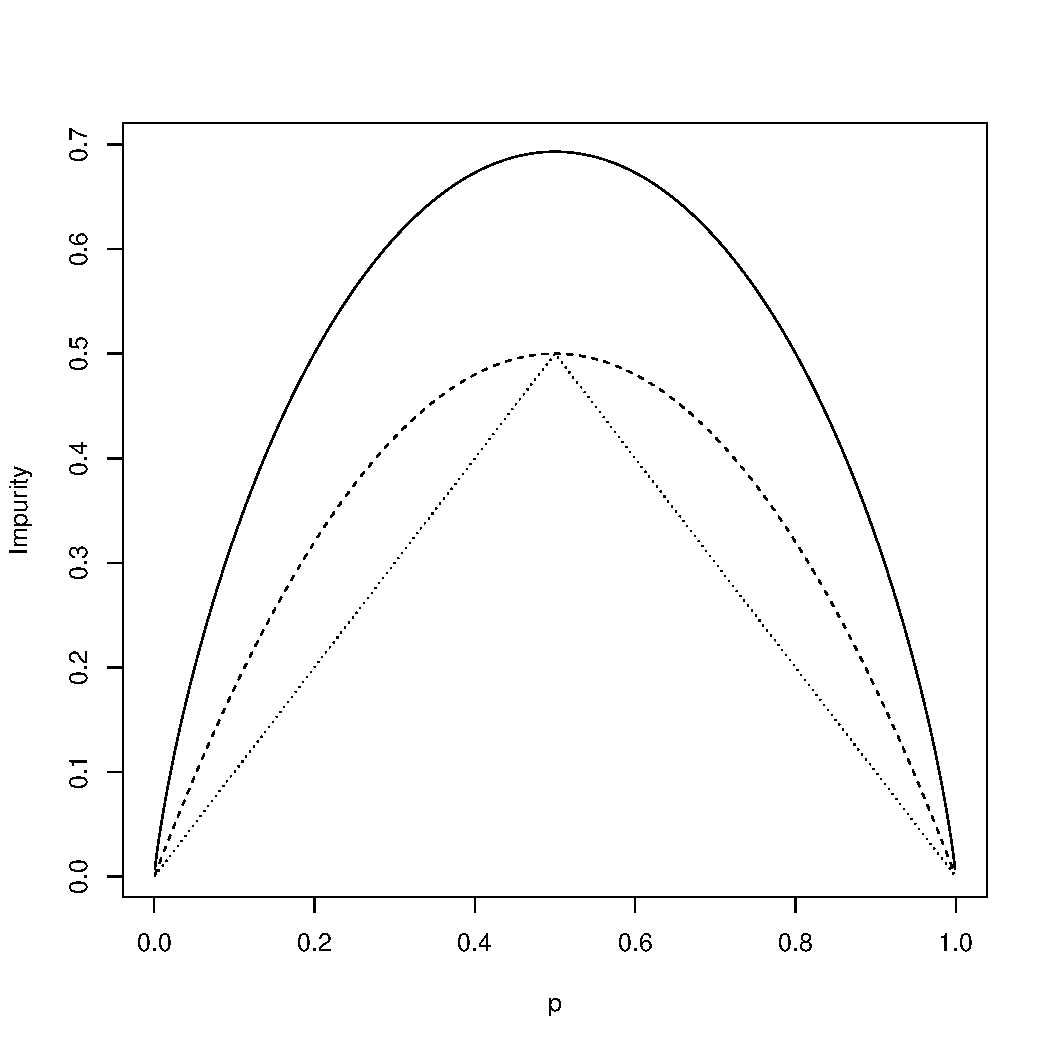
\includegraphics[scale=.7]{figures/impurity_plot.pdf}
  \caption{A plot of the three impurity functions: entropy (solid line), Gini (thatched line), and misclass probability (dots).  }
  \label{fig:impurity}
\end{figure}

To build a regression tree, in place of an impurity function, we use the mean squared error criteria denoted

$$\text{MSE}: \phi(y_i, \bar{y})=\frac{\sum_{i=1}^n(y_i-\bar{y})^2}{n}.$$
The reader should note that the greedy approach to decision tree induction always tries to optimize impurity functions. The optimization problems are known to be NP-Hard (for an introduction to complexity theory confer Garey and Johnson \cite{garey1979computers}). Briefly, NP-Hard optimization problems are considered some of the hardest optimization problems to solve. These optimization problems increase exponentially with the number of observations in the problem. Therefore, exact methods will nearly always take too long to compute and thus greedy strategies are used to approximate the global optimum, assuming one exists, with a local optimum. 
\subsection{Induction}
The induction of decision trees proceeds by solving the objective function

\begin{equation}
\underset{t,s}{argmax} \Delta\phi = \phi - \pi_L\phi_L-\pi_R\phi_R.
\end{equation}
Here the variables $t$ and $s$ scroll over all covariates in the data and all midpoints between successive observations (or at observed points) of the $t$th covariate respectively. The proportions $\pi_L$ and $\pi_R$ represent the number of data points going into the node to the left ($L$) and right ($R$) of the current node if the chosen split is on covariate $t$ and observation $s$. The impurity functions are similarly subscripted. Thus, if there are 100 observations in the current node and as a result of the split on covariate $t$, at observation $s$, 70 observations go into the left child node and 30 observations go into the right child node, then the two proportions are $(\pi_L, \pi_R) = (0.7, 0.3)$. 

The tree induction process continues until no more data points are incorrectly classified, or a predetermined stopping rule is met. A common stopping rule is to stop when there are less than $5$ observations in a terminal node. Once the full tree has been built, the second stage of the process now starts. This is known as the pruning stage. Now that the full tree is grown, we progressively prune back terminal nodes of the tree until the root node occurs. Several related approaches have been proposed in the literature to select the optimal tree via pruning. The most common is to select the tree using the regularized risk estimate given in Equation \ref{eqn:reg_risk_est} \newnot{symbol:risk_tree}

\begin{equation}\label{eqn:reg_risk_est}
R(\mathcal{T}_i,\alpha) = R(\mathcal{T}_i) + \alpha \vert \mathcal{T}_i \vert. 
\end{equation}

Here the $\alpha$ parameter is a regularization parameter with larger values of $\alpha$ given greater penalty to the number of terminal nodes in the tree, here denoted $\vert \mathcal{T}_i\vert$. The notation $R(\mathcal{T}_i)$ denotes the risk of the tree, which is usually calculated as the sum of squared errors across all terminal nodes in a regression setting or the sum of the impurity function values in each terminal of the tree in the classification case. We choose the value of $\alpha$ leading to the smallest regularized risk ($R(\mathcal{T}_i,\alpha)$).  The value of $\alpha$ is chosen over a grid of positive values by minimizing Equation \ref{eqn:reg_risk_est} on holdout data, using a cross validation approach, 

Discussion of consistency of this pruning rule can be found in Devroye et al. \cite{devroye1996probabilistic}, Breiman et al. \cite{breiman1984classification}, Gey \cite{gey2005model}, and Suav\'{e} and Tuleau-Malot \cite{sauve2011variable}. All the theoretical results require controlling the complexity of the decision tree, $\vert\mathcal{T}\vert$, and allowing the number of data points $n\to\infty$. However, the results in Devroye et al. \cite{devroye1996probabilistic} also give explicit bounds for the error of decision tree classifiers for finite values of $n$. 

The pruning rule discussed here, and the induction process overall, is an implicit form of model selection. This is implicit because the selected variables are the variables left in the tree after pruning. Those variables considered important are the variables that remain and those variables not selected are considered not important. Breiman et al. \cite{breiman1984classification} define no measure of importance on each variable, so it is difficult to rank variables based on importance. Breiman \cite{breiman2001random} proposed such a measure, called variable importance (abbreviated VIMP) \newabbrev{abbrev:VIMP} but in the context of random forests and not for a single decision tree. We propose different methods to perform explicit variable selection for Bayesian decision trees in later chapters.   

\subsection{A Simple Example}

In this subsection we work through a simple example to give the reader a flavor of the calculations necessary to induct a decision tree. 

Consider the following data 

\begin{table}[H]
\begin{center}
\begin{tabular}{ l | c | c | c }
  i& $y_i$ & $x_1$ & $x_2$\\
  \hline
  1&1 & 2 & 3 \\
  2&2 & 5 & 6 \\
  3&5 & 8 & 9 \\
\end{tabular}
\caption[A simple decision tree example data]{A simple decision tree example data.}
\label{fig:dtree_firststep}
\end{center}
\end{table}

We have three observations and two covariates within each observation. The response is a continuous random variable, so this will be a regression tree approach. We will examine potential split points by looking at the midpoints between two observed values of the covariates. We begin by sorting the data in increasing order for both covariates. Fortunately, in this case, the data is already in order for both covariates, so no sorting is necessary. We now examine the possibility of a split point on $x_1$. Using the MSE \newabbrev{abbrev:MSE} impurity we calculate $\phi$, $\phi_L$, and $\phi_R$. A sum of squared error calculation shows $\phi = 26/3$, which is a constant value for all calculations we perform. 
Now for a split between observation 1 and 2,
$$
\Delta\phi=26/3- (1/3)(1-1)^2 - (2/3)((2-7/2)^2+(5-7/2)^2)=26/3-9/3=17/3.
$$ 
For a split between observation 2 and 3, 
$$
\Delta\phi=26/3 - (2/3)( (1-3/2)^2 + (2-3/2)^2)  - (5-5)^2(1/3)= 26/3-1/3=25/3 
$$ 
Now, because the data is sorted, the same $\Delta\phi$ values will result for potential splits on $x_2$. Therefore, we, somewhat arbitrarily, choose to split on the covariate with the smaller index, $x_1$. Thus, our first split is on the value $\{x_1: x_1 \leq 6.5\}$ and the tree at this point looks like that in Figure \ref{fig:dtree_firststep}. Note that Figure \ref{fig:dtree_firststep} displays the mean of the values in each terminal node. The mean value is the predicted value for observations falling into the given terminal node.

\begin{figure}
\begin{center}
\tikzset{every tree node/.style={minimum width=4em,draw,circle},
         blank/.style={draw=none},
         edge from parent/.style=
         {draw, edge from parent path={(\tikzparentnode) -- (\tikzchildnode)}},
         level distance=3cm}
\begin{tikzpicture}
\Tree
[. $x_1\leq 6.5$     
    [.7/2 ]
    [.5  
    \edge[blank]; \node[blank]{};
            ]
    ]
]
\end{tikzpicture}
\end{center}
\vspace{-3.5cm}
\caption[A simple decision tree]{The decision tree after the first split.}
\label{fig:dtree_firststep}
\end{figure}
If we had more than $3$ observations, we would then continue calculating $\Delta\phi$s for the data that falls into each of the two resultant terminal nodes, continuing until there is only one observation in each terminal node, or until there is some specified number of observations in each terminal node. Although any number is possible, the specified minimum number of observations in each terminal node is usually 5. Once this process is completed, the induction step is finished, and the pruning process begins. 

\section{Bayesian Approaches}
\label{ch:p2sub_bayes}

This section describes a Bayesian approach to decision trees. In the previous chapter we presented a greedy algorithm to fit decision trees. Besides the observed error in a greedy decision tree, there is nothing to describe the fit of the model, or to  provide a measure over the decision tree. This section provides both of these quantities. We begin by defining the CGM model and calculating necessary quantities for the algorithm. Furthermore, there is no explicit model selection, which will be the main contribution of this thesis.    

\subsection{The CGM approach}
We begin by defining notation and measures on each quantity of the tree. 
We assume that the tree topology and split rules are conditionally independent. Based on fundamentals of probability we have the following relationships

\begin{align}
 \Pr(\mathcal{T}_i \vert \yvec, X ) &\propto \Pr(\mathcal{T}_i)\Pr(\yvec \vert \mathcal{T}_i, X)\nonumber \\
  &\propto \Pr(\mathcal{T}_i)\int_{\Theta}\Pr(\yvec \vert \mathcal{T}_i, X, \theta)\pi(\theta)d\theta,
\end{align}
where $\Pr(\mathcal{T}_i)$ denotes the prior measure on trees and $\Pr(\yvec \vert \mathcal{T}_i, X)$ denotes the integrated likelihood of the tree. Finally, $\Pr(\yvec \vert \mathcal{T}_i, X, \theta)$ and $\pi(\theta)$ denote the tree likelihood and the prior measure on node parameters, respectively. CGM \cite{chipman1998bayesian} defined this  conditional decomposition and showed how to use this to construct an algorithm to sample Bayesian decision trees. We now define the aspects of the model described in the CGM paper \cite{chipman1998bayesian}. 

The decision tree model has two main components, the tree $\mathcal{T}$ with $b$ terminal nodes, and the parameters in each terminal node, $(\theta_1,\dots,\theta_b)$. 
The two main likelihoods in each terminal node are the normal and the multinomial, for continuous and categorical responses, respectively. 
We denote the responses in each terminal node as the vector  of vectors $Y\equiv (Y_1, \dots, Y_b)$. Then $Y_i = (y_{i1}, \dots y_{in_i})$ and the main relation is the independence breakdown 
\begin{equation}
f(Y\vert \mathcal{T}, X, \theta) =\prod_{i=1}^b f(Y_i\vert \mathcal{T}, X, \theta_i) = \prod_{i=1}^b \prod_{j=1}^{n_i} f(y_{ij} \vert \mathcal{T}, X, \theta_i).
\end{equation}
The two likelihoods are given by
\begin{equation}
f(y_{ij} \vert \mathcal{T}, X, \theta_i) = N(\mu_i,\sigma_i),
\end{equation}
and the multinomial likelihood is
\begin{equation}\label{eqn:mult_lhood}
f(y_{i1}, \dots ,y_{in_i} \vert \mathcal{T}, X, \theta_i) = \prod_{j=1}^{n_i}\prod_{k=1}^K p_{ik}^{\mathds{1}(y_{ij}=k)}.
\end{equation}
In Equation \ref{eqn:mult_lhood}, $p_{ik}$ denotes the probability $y_{ij}$ of being in category $k$ in terminal node $i$ and $\mathds{1}(A)$ denotes the indicator function for the set $A$. 

We now proceed to define the tree prior. We start with a tree consisting of a single node, the root node. We then imagine the tree growing by randomly choosing terminal nodes to split on. To grow a tree we must specify two functions, the growing function and the splitting function.  The splitting function is denoted $p_{\text{split}}(\eta, \mathcal{T})$ and the rule function is denoted $p_{\text{rule}}(\rho \vert \eta, \mathcal{T})$. The rule function provides a criteria to determine which of the two child nodes the observed data go into. If the observed covariate value is less than the rule value, then the observation go into the left child node. Similarly, if the observed covariate value is greater than the rule value, then that observation goes into the right child node. Growing a tree (called induction) consists of iterating these steps. creating two new children from a terminal node and assigning a rule to the terminal node (now a parent of two terminal nodes). Figure \ref{fig:induction_firststep} illustrates one iteration of the induction process graphically. 

\begin{figure}
\begin{center}
\subfigure{
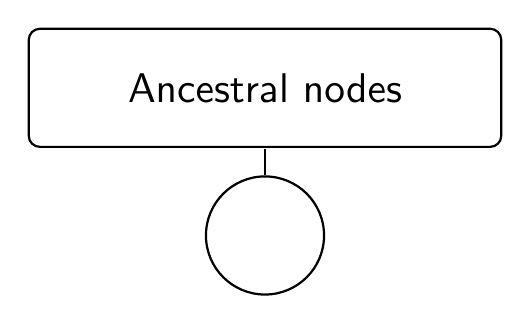
\begin{tikzpicture}[
    scale = 1.5, transform shape, thick,
    every node/.style = {draw, circle, minimum size = 10mm},
    grow = down,  % alignment of characters
    level 1/.style = {sibling distance=3cm},
    level 2/.style = {sibling distance=4cm}, 
    level 3/.style = {sibling distance=2cm}, 
    level distance = 1.25cm
  ]
  \node[shape = rectangle, rounded corners,
    minimum width = 4cm, font = \sffamily] {Ancestral nodes} 
  child { node (Start){}};
  \begin{scope}[nodes = {draw = none}]
    \begin{scope}[nodes = {below = 11pt}]
      \end{scope}
  \end{scope}
\end{tikzpicture}
}
\subfigure{
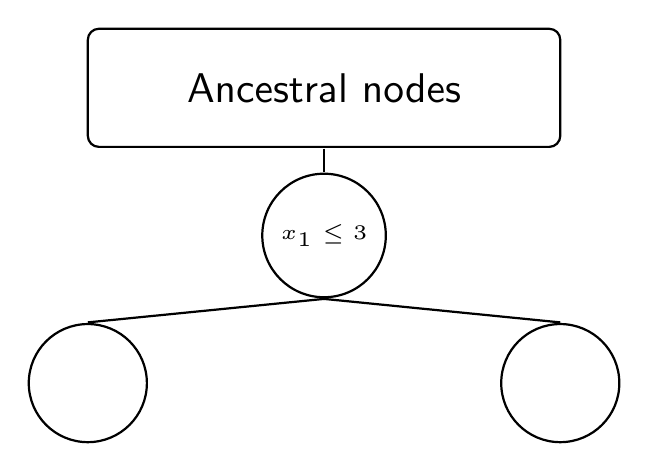
\begin{tikzpicture}[
    scale = 1.5, transform shape, thick,
    every node/.style = {draw, circle, minimum size = 10mm},
    grow = down,  % alignment of characters
    level 1/.style = {sibling distance=3cm},
    level 2/.style = {sibling distance=4cm}, 
    level 3/.style = {sibling distance=2cm}, 
    level distance = 1.25cm
  ]
  \node[shape = rectangle, rounded corners,
    minimum width = 4cm, font = \sffamily] {Ancestral nodes} 
  child { node (Start){\tiny{$x_1 \leq 3$}}
   child {   node (A) {}
       }
   child {   node  (D) {}
     }
  };
  \begin{scope}[nodes = {draw = none}]
    \path (Start) -- (A) node [near start, left]  {};
      \path (Start) -- (D) node [near start, right] {};
    \begin{scope}[nodes = {below = 11pt}]
      \end{scope}
  \end{scope}
\end{tikzpicture}
}
\end{center}
\caption[Illustrating the induction process]{A terminal node in the decision tree before (left) and after (right) a split on a terminal node.}
\label{fig:induction_firststep}
\end{figure}

The probability measure on the potential splits of the tree is
\begin{equation}\label{eqn:psplit}
p_{\text{split}}(\eta, \mathcal{T})=\alpha(1+d_{\eta})^{-\beta}, \ \ \alpha>0, \beta\geq 0,\\
\end{equation}
where $d_{\eta}$ denotes the depth of the node $\eta$ and $\alpha$, and $\beta$ are scalars. The probability of the specific rule, denoted $\rho$ is 
\begin{equation}\label{eqn:prule}
p_{\text{rule}}(\rho \vert \eta, \mathcal{T}) \propto \underbrace{\Pr(\text{split on covariate})}_{=p_{\text{split}}}\underbrace{\Pr(\text{split on a value given a covariate})}_{=p_{\text{rule}}}. 
\end{equation}

Here CGM recommends using a discrete uniform prior on $p_{\text{split}}$ and splitting uniformly amongst the splitting values (in $p_{\text{rule}}$) that do not result in an empty terminal node. While we choose the same proposal mechanism for the $p_{\text{rule}}$ quantity, the main point of this thesis is to examine and propose alternate specifications for $p_{\text{split}}$. The data sets modeled in CGM \cite{chipman1998bayesian} and DMS \cite{denison1998bayesian}, and other modifications in the literature, deal with data with a small number of predictors. In this thesis we are concerned with a large number of predictors, so we will focus on variable selection, which will ultimately explain how we specify quantity $p_{\text{split}}$ in Equation \ref{eqn:prule}. 

\subsection{Integrated Likelihood}
We will now focus on the integrated likelihood, which is the quantity 

\begin{equation}\label{eqn:int_lhood}
\Pr(Y_i \vert \mathcal{T}, X) = \int_{\Theta}\Pr(Y_i \vert \mathcal{T}_i, X, \theta)\pi(\theta)d\theta.
\end{equation}
To evaluate the integral in Equation \ref{eqn:int_lhood} we must first define a prior, denoted $\pi(\theta)$, for the parameters in each terminal node. 
There are two possible priors for the case of the normal likelihood that will result in a conjugate prior/posterior. These are normal and normals-gamma distributions, or equivalently, normal-inverse gamma distributions depending upon the given parametrization. 

\subsection{The Process Prior}

Assuming we have a closed form solution for the integral in Equation \ref{eqn:int_lhood}, we can use Bayes' rule to determine 
\begin{equation}\label{eqn:tree_post}
\Pr(\mathcal{T} \vert Y , X) \propto \Pr(Y \vert X ,\mathcal{T})\Pr(\mathcal{T}).
\end{equation} 
We now have an effective means of searching the posterior space over trees to determine the high posterior trees. We can do so by using the Metropolis-Hastings rule 

\begin{equation}\label{eqn:MHrule}
\mathcal{T}^{i+1} =\begin{cases}
\mathcal{T}^*, & \text{with probability}\ \alpha(\mathcal{T}^*, \mathcal{T}^i) = \text{min}\left(\frac{q(\mathcal{T}^*, \mathcal{T}^i)}{q(\mathcal{T}^i, \mathcal{T}^*)}\frac{\Pr(Y\vert X, \mathcal{T}^*)}{\Pr(Y\vert X,\mathcal{T}^i)}\frac{\Pr(\mathcal{T}^{*})}{\Pr(\mathcal{T}^i)},1 \right) \\
\mathcal{T}^{i}, & \text{with probability}\ 1-\alpha(\mathcal{T}^*, \mathcal{T}^i).
\end{cases} \end{equation}

To evaluate the normalization constant would require summing Equation \ref{eqn:tree_post} across all possible trees. This sum includes $\mathcal{O}(nd\frac{4^h}{h^{3/2}})$ terms, with $h$ denoting the maximum height of the trees, $n$ denoting the number of observations, and $d$ denoting the number of covariates. This is an infeasible sum for most data sets, and for all data sets examined in this thesis. For the function $q(-\vert-)$, which is called the proposal function, we use $q$ to propose a new tree $\mathcal{T}^*$.   
In Equation \ref{eqn:MHrule}, $q(\mathcal{T}^*\vert\mathcal{T})$ denotes proposing a new tree $\mathcal{T}^*$, starting from the current tree $\mathcal{T}$. 
 Our proposal mechanism is as follows:
  \begin{itemize}
 \item The grow step chooses at random one of the terminal nodes and proposes to append two new child nodes with a certain probability that could depend on the tree depth, splitting on a chosen covariate.
 \item The prune step works in reverse of the grow. A terminal node is selected at random and that node and the node's sibling are pruned to the immediate parent of the two child nodes.
 \item The change step randomly picks an internal node and attempts to change the split rule at the node with that of another observation, possibly on a different covariate.
  \item The swap step randomly selects an internal node that is not the root node and proposes to swap the split rules of the parent-child pair. If both child nodes split on the same covariate, then both the children and the parent node's rules are swapped.
  \item The rotate step randomly chooses a left or right rotation move. Then this step randomly chooses an admissible internal node and rotates.
 \end{itemize}
  The rotate operation for binary trees was first introduced in Sleater and Tarjan \cite{sleator1985self} and was introduced into Bayesian decision trees in GL \cite{gramacy2008bayesian}. A good introduction and several practical uses of the rotate move can be found in Cormen, Lieserson, Rivest and Stein \cite{cormen2001introduction}. The proposal of Gramacy and Lee \cite{gramacy2008bayesian} only allows a rotate move for the specific case when a swap move is proposed and the parent child pair both split on the same covariate. We modify this rule and allow rotate to be a separate operation of the transition kernel and not a special swap move case. The proposal mechanism of CGM uses the grow, prune, change and swap moves only. We also allow swap moves in our proposal. In addition, neither of CGM nor Gramacy and Lee \cite{gramacy2008bayesian} included weights on each covariate in their examples or model specifications. CGM sampled each covariate and split value uniformly, at random. 
  
 The probability measure on the tree is  
 
 \begin{equation}
 \Pr(\mathcal{T}) = \prod_{\eta \in \mathcal{N}} p_{\text{rule}}(\rho \vert \eta, \mathcal{T})p_{\text{split}}(\eta, \mathcal{T}),
\end{equation}
where $\mathcal{N}$ denotes the set of nodes in tree $\mathcal{T}$.
The probability measure on each split, here denoted $p_{\text{split}}(\eta, \mathcal{T})$, uses Equation \ref{eqn:psplit}. Similarly, the measure on each rule, here denoted $p_{\text{rule}}(\rho \vert \eta, \mathcal{T})$, uses Equation \ref{eqn:prule}. 
All that is left to specify is the likelihood in each node and the prior structure for the parameters in each node, both of which are done in the next subsection. 

\subsection{Node Likelihoods and Priors}

CGM discuss three models. Two of the models use Gaussian priors and Gaussian likelihoods and one of the models uses a Dirichlet prior and a multinomial likelihood. The two Gaussian models differ in that one has a single variance and the other has a different variance for each node. As noted by Lee \cite{lee2006decision}, in a greedy optimization context, sometimes the data suggest a different model than either a Gaussian or a multinomial-Dirichlet. If the experiment suggests analyzing data using an alternate model, the Bayesian context easily handles these alterations, once the corresponding likelihood and prior are specified. Lee \cite{lee2006decision}, proposed a zero inflated poisson (ZIP) model to analyze the solder data. Note our Bayesian model can easily handle extensions such as ZIP response data and also permits covariate selection, provided the integrated likelihood is available in closed form.

We begin with the Gaussian likelihood and Gaussian prior model. We define the likelihood as 
\begin{equation}\label{eqn:norm_lhood1}
N[y_{ij} \vert \mu_i, \sigma^2].
\end{equation}
Also, we define the prior for $\mu_i$ as 
\begin{equation}\label{eqn:norm_prior1}
N[\mu_i\vert \bar{\mu}, \sigma^2 ].
\end{equation}
Furthermore, we define the prior for $\sigma^2$ as 
\begin{equation}\newnot{symbol:inv_gamma}
\text{Inv-Gamma}(\sigma^2\vert \alpha, \beta).
\end{equation}
All that remains is to evaluate the integral 
\begin{equation}\label{eqn:int_model1}
\prod_{i=1}^b \int_0^\infty \int_{-\infty}^{\infty} \prod_{j=1}^{n_i} N[y_{ij} \vert \mu_i, \sigma^2]N[\mu_i\vert \bar{\mu}, \sigma^2 ]\text{Inv-Gamma}(\sigma^2\vert \nu/2, \nu\lambda/2)d\mu_id\sigma^2.
\end{equation}
For the Gaussian prior and likelihood we can explicitly calculate the marginal likelihood. Being able to marginalize the node parameters explicitly allows us to implement a Metropolis-Hastings algorithm without resorting to complicated, specialized algorithms, or numerical integrations. Straightforward analytic manipulations yield the solution to Equation \ref{eqn:int_model1} written in Equation \ref{eqn:int_model1_soln}
\begin{equation}\label{eqn:int_model1_soln}
\frac{ca^{b/2}}{\prod_{i=1}^b\sqrt{n_i+a}}\times \left(\sum_{i=1}^b\left(\sum_{j=1}^{n_{i}}(y_{ij}-\bar{y}_i)^2\right)+ \frac{(\bar{y}_i -\bar{\mu})^2(n_ia)}{n_i+a} \right)^{-(\nu+n)/2}\hspace{-1.4cm}.
\end{equation}
If we assume instead that the variances might change from node to node, then the stated model is misspecified. Let us denote the variance in each node as $\sigma_i^2$ and keep all other notations from the stated model specification. Then the model is specified using 
\begin{equation}\label{eqn:normal_likelihood_many_variance}
N[y_{ij} \vert \mu_i, \sigma_i^2].
\end{equation}
Also, we define the prior for $\mu_i$ as 
\begin{equation}\label{eqn:multi_variance_prior}
N[\mu_i\vert \bar{\mu}, \sigma_i^2 ].
\end{equation}
Furthermore, we define the prior for the $\sigma_i^2$s as 
\begin{equation}\label{eqn:sigma_priors}
\text{Inv-Gamma}(\sigma_i^2\vert\nu/2, \nu\lambda/2)
\end{equation}
 and now we evaluate the integral equation 
 \begin{equation}\label{eqn:int_model2}
\prod_{i=1}^b \int_0^\infty \int_{-\infty}^{\infty} \prod_{j=1}^{n_i} N[y_{ij} \vert \mu_i, \sigma_i^2]N[\mu_i\vert \bar{\mu}, \sigma_i^2 ]\text{Inv-Gamma}(\sigma_i^2\vert \nu/2, \nu\lambda/2)d\mu_id\sigma_i^2. 
\end{equation}
The result of computing the integrals in Equation \ref{eqn:int_model2} is 
\begin{equation}\label{eqn:int_model3}
\prod_{i=1}^b\pi^{n_i/2}(\lambda\nu)^{\nu/2}\sqrt{\frac{a}{n_i+a}}\frac{\Gamma((n_i+\nu)/2)}{\Gamma(\nu/2)}\times \left( \sum_{j=1}^{n_{i}}(y_{ij}-\bar{y}_i)^2+ \frac{(\bar{y}_i -\bar{\mu})^2(n_ia)}{n_i+a}+\nu\lambda  \right)^{(n_i+\nu)/2}.
\end{equation}
These are the two ``regression'' models for the Bayesian decision trees given in CGM \cite{chipman1998bayesian}. 

The classification model discussed in CGM \cite{chipman1998bayesian} defines the likelihood, prior, and integrated likelihood as
\begin{equation}
y_{i1}, \dots, y_{in_i} \vert \mathcal{T} \sim \text{Multinomial}(Y_i \vert \vec{n}, \vec{p}),\newnot{symbol:mult}
\end{equation} 
\begin{equation}
\vec{p} \vert \mathcal{T} \sim \text{Dirichlet}(\vec{p}\vert \vec{\alpha}), \newnot{symbol:dirichlet}
\end{equation} 
and
\begin{equation}\label{eqn:int_model4}
\Pr(Y\vert \mathcal{T}, X)=\left(\frac{\Gamma(\sum_{k=1}^K\alpha_k)}{\prod_{k=1}^K\Gamma(\alpha_k)} \right)^b \prod_{i=1}^b\left( \frac{\prod_{k=1}^K\Gamma(n_{ik}+\alpha_k)}{\Gamma(n_i +\sum_{k=1}^K\alpha_k)} \right),
\end{equation} 
respectively. 
 
If we wanted to model the data using a different data generating process, for example a zero-inflated Poisson, we could do so by specifying a different likelihood, prior, and by computing the integrated likelihood. For a zero-inflated Poisson model defining a likelihood, prior, and calculating the integrated likelihood is possible using gamma priors for the rate ($\lambda$) and beta priors for zero inflation components ($\phi$). 
 
 \subsection{A Bayesian Zero Inflated Poisson Model}
 %\textbf{Write out the details of this model here and cite applied statistics paper which uses a greedy approach.}
 
 Lee and Jin \cite{lee2006decision} reconsidered impurity functions in light of the connection to likelihood functions. Lee and Jin \cite{lee2006decision} proposed to use likelihood functions instead of impurity functions that model the data generating process. Towards this end they considered the soldering data from Chambers and Hastie \cite{chambers1992statistical}. The response of interest in this case is a collection of counts on manufactured circuit boards. This response has many zero values and Lee and Jin \cite{lee2006decision} proposed using a zero inflated (ZIP)\newabbrev{abbrev:ZIP} Poisson likelihood to model the measured counts. Lee and Jin \cite{lee2006decision} optimized using a greedy algorithm and they found the fit and holdout prediction to be better using the ZIP model in each terminal node. If we are to use a Bayesian approach to this problem, we need to define the likelihood, the prior, and the integrated likelihood. We now define these three quantities.
 
 The likelihood for a single observation is 
 \begin{equation}
 f(y\vert \lambda, \phi) \propto \mathds{1}(y=0)\left(\phi + (1-\phi)\exp{(-\lambda)}\right) + \mathds{1}(y>0)\left(\exp{(-\lambda)}\frac{\lambda^y}{y!}\right).
 \end{equation}
 The priors for $\lambda$ and $\phi$ are
 \begin{equation}
 \pi(\phi, \lambda)\propto \underbrace{\frac{\phi^{\alpha-1}(1-\phi)^{\beta-1}\Gamma(\alpha+\beta)}{\Gamma(\alpha)\Gamma(\beta)}}_{=\text{A beta prior }} \times \underbrace{\frac{ \lambda^{\alpha_{\lambda}-1}\exp{(-\lambda/\beta_{\lambda})} }{\Gamma(\alpha_{\lambda})\beta_{\lambda}^{\alpha_{\lambda}}}}_{=\text{A gamma prior}}.
 \end{equation}

 Now we need to calculate the integrated likelihood, which means that we must evaluate 
 \begin{align} \hspace{-.9in}
 &\int_0^1\int_0^\infty \left(\mathds{1}(y=0)\left(\phi + (1-\phi)\exp{(-\lambda)}\right) + \mathds{1}(y>0)\left(\exp{(-\lambda)}\frac{\lambda^y}{y!}\right)\right) \\ \nonumber
 & \frac{\phi^{\alpha-1}(1-\phi)^{\beta-1}\Gamma(\alpha+\beta)}{\Gamma(\alpha)\Gamma(\beta)} \times \frac{ \lambda^{\alpha_{\lambda}-1}\exp{(-\lambda/\beta_{\lambda})} }{\Gamma(\alpha_{\lambda})\beta_{\lambda}^{\alpha_{\lambda}}}d\lambda d\phi.
 \end{align}
 
 Let $j$ index the observed zero counts. Furthermore, let $\bar{y}_{+}$ denote the average of the non-zero counts and $n_0$ and $n_+$ denote the number of zeros and non-zeros in the data respectively. 
 Now we assume that the observations are $i.i.d.$ and simple calculations lead to the conclusion that
 
 \begin{align}\label{eqn:zip_int_lhood}\hspace{-.7in}
 \Pr(Y\vert X, \mathcal{T})& = \left[\sum_{j=0}^{n_0} {n_0 \choose j}\frac{\Gamma(\alpha+\beta)\Gamma(\alpha+j)\Gamma(n_0+\beta-j)}{\Gamma(\alpha)\Gamma(\beta)\Gamma(\alpha+\beta+n_0)}\left(\frac{n_0-j+\beta_{\lambda}^{-1}}{\beta_{\lambda}}\right)^{\alpha_{\lambda}} \right] \\ \nonumber
 & + \frac{\Gamma(\alpha_{\lambda}+n_+\bar{y}_+)}{\Gamma(\alpha_{\lambda})\beta_{\lambda}^{\alpha_{\lambda}}}\left(n_+ + 1/\beta_{\lambda} \right)^{\alpha_{\lambda}+n_+\bar{y}_+}.
\end{align}

A similar calculation may be performed for a response variable that is distributed as a zero-inflated negative binomial random variable (ZINB).\newabbrev{abbrev:ZINB}
 
\section{Previous Variable Selection}
\label{ch:p4sub_var_sel}

Previous approaches to variable selection have focused primarily on the linear model or GLM or GLMM models, all of which we briefly reviewed in Chapter \ref{ch:intro}. Hereafter we will refer to all three types of models as linear. The correspondence between variable selection in linear models and in Bayesian decision trees is a simple correspondence between zeros in the linear model, or zero means of the normal and transformed values on the unit simplex. This correspondence will be detailed in the next subsection of this chapter.   

Ishwaran et al. \cite{ishwaran2010high} propose a modification to Variable Importance (VIMP) criteria that allows some very basic theory to describe the VIMP's analytical properties. VIMP was first proposed by Breiman \cite{breiman2001random} as a method to assess which covariates are important in a dataset. The difficulty with both Ishwaran et al's method and Breiman's method is that they are both very much black box techniques. VIMP basically takes a split in a decision tree on a specific covariate and randomly decides if the observation should go to the left or the right child node. This is done for a collection of observations and the random predictions are averaged against the actual predictions. The resulting numeric estimates for each covariate are the VIMP estimates. A ranking of these values provides a ranking of the covariates. 

A similar method of ranking covariates was proposed by Taddy, Gramacy, and Polson \cite{taddy2011dynamic}. Taddy, Gramacy and Polson proposed a Bayesian approach and used the Bayesian equivalent to $\Delta\phi$ from this chapter, written here for clarity, 
\begin{equation}
\Delta\phi = \int\phi ds - \pi_L\int\phi ds -\pi_R \int \phi_Rds. 
 \end{equation}
Taddy, Gramacy and Polson proposed using samples and estimating the integrals with Monte Carlo approximations. In this case the approach is using a greedy measure on a Bayesian problem, something we find confusing.
In the Bayesian approach the quantity $\Delta\phi$ has little meaning, because we are using an MCMC approach to search across trees. The resulting estimates of the covariates' importance will be the same as the greedy approach, which we find undesirable for many reasons. The method proposed by Taddy, Gramacy, and Polson is worth comparing against our approach because it will have similar difficulties to CGM in high-dimensional data. We will do compare their approach to a time series version of our model in future work.
 

 
%\textbf{Write in a brief description of both Ishwaran et al approach and Gramacy and Lee approach}. 

%% previous variable selection details file

\subsection{Normal Distributions Transformed to the Unit Simplex: The ALoVaS method. }\label{sec:ALN_chapter}

This chapter outlines the additive logistic transformation, which transforms a $d$ dimensional multivariate normal distribution onto the unit simplex in $d+1$ dimensions. Note that the unit simplex in $d+1$ dimensions actually lies in a subspace of $d$ dimensions because of the constraint that the sum of the probabilities equals one. 

The goal of this chapter is to find a transform that moves the space $\mathbb{R}^d$ \newnot{symbol:real} to the simplex $\mathbb{S}^d$. \newnot{symbol:simp} The simplex $\mathbb{S}^d$ is a space defined by the constraints $\{x_i: 0<x_i<1, \sum_{j=1}^dx_j <1 \}$, and the extra term $x_{d+1}=1-\sum_{j=1}^d x_j$ ensures the total sums to 1.  

Define the notation $\yvec$, for the normal random variables that reside in the $\Rsp{d}$  dimensional space. Define the notation $\xvec$  for the vector that resides on $\simp{d}$, the simplex in $d$ dimensions. We use an underline to indicate that the stated quantity is a column vector and capital greek letters (and $I$) will denote matrices (the identity matrix) 

\begin{equation}\label{eqn:simplex_transform}
x_i = \frac{e^{y_i}}{1+\displaystyle{\sum_{j=1}^de^{y_j}}}. \\
\end{equation}
The Jacobian of the transform is defined as
\newnot{symbol:jacobian}
\begin{equation}\label{eqn:jacobian}
J(\yvec \vert \xvec) = \left( \prod_{j=1}^{d+1}x_j \right)^{-1}.
\end{equation}

It is important to note that $\yvec\in\Rsp{d}$, whereas $\xvec\in\simp{d}$. The $d$ dimensional normal has the usual parameters and density

\begin{equation}\label{eqn:multinormal}
f_{\yvec}(\yvec\vert \Sigma, \mu)=(2\pi)^{-d/2}|\Sigma|^{-1/2}\exp{\left(-1/2(\yvec-\muvec)^T\Sigma^{-1}(\yvec-\muvec)\right)}.
\end{equation}

Upon applying the transformation defined by Equation \ref{eqn:simplex_transform}, we arrive at the additive logistic normal (ALN) distribution, with density 

\begin{equation}
f_{\xvec}(\xvec\vert \Sigma, \mu)=\frac{(2\pi)^{-d/2}}{\sqrt{\vert\Sigma\vert}\prod_{j=1}^{d+1}x_j } 
\exp{\left(-1/2(\text{log}(\xvec_{(d+1)}/x_{d+1})-\muvec)^T\Sigma^{-1}(\text{log}(\xvec_{(d+1)}/x_{d+1})-\muvec)\right)}.
\end{equation}
The vector notation $\xvec_{(d+1)}$ denotes the vector in $d$ dimensions that has the $d+1$ entry removed from the vector $\xvec$. 
It is important to note that this density function is defined on the space $\simp{d}$ and \emph{not} on the space $\Rsp{d}$. 

A useful property of this transform is that we can handle probabilities defined on the $d$ dimensional simplex while working with a normal distribution. This is a common and comfortable probability distribution for most statisticians and applied scientists.
We now wish to understand how the specification of the mean vector $\muvec$ and the covariance matrix $\Sigma$ impact the structure of the ALN density. From simulation we can formulate the following conclusions: 

\begin{itemize}
\item With $\Sigma=I$, increasing the mean vector in the positive direction in any one of the $d$ components individually corresponds to shifting density towards the corner of the simplex associated with that covariate. 
\item With $\Sigma=I$, increasing the mean vector in the negative in \emph{all} $d$ components corresponds to shifting density towards the $d+1$ corner of the simplex. 
\item Keeping $\muvec =\vec{0}$, adjusting any of the variances corresponds to shifting towards a projected space of $\simp{d}$. 
\item With $\muvec =\vec{0}$, making one variance small corresponds to the shifting density towards the median of the simplex associated with the remaining $d$ dimensions. 
\item Making the $\Sigma$ matrix approximately singular and moving $\muvec$ in the negative direction for all components places most of the probability density along the median of simplex associated with first $d$ dimensions. 
\item If $\Sigma = \text{Diag}(\sigma^2_j)$,\newnot{symbol:diag} as the $\sigma^2_j$ entries become smaller, the probabilities approach the CGM specification.    
\end{itemize}

Using the transformation defined in Equation \ref{eqn:simplex_transform} and the fact that it is relatively simple to simulate from the vector normal distribution, the ALN density can be simulated. 

\begin{figure}[ht]
\begin{minipage}[b]{0.45\linewidth}
\centering
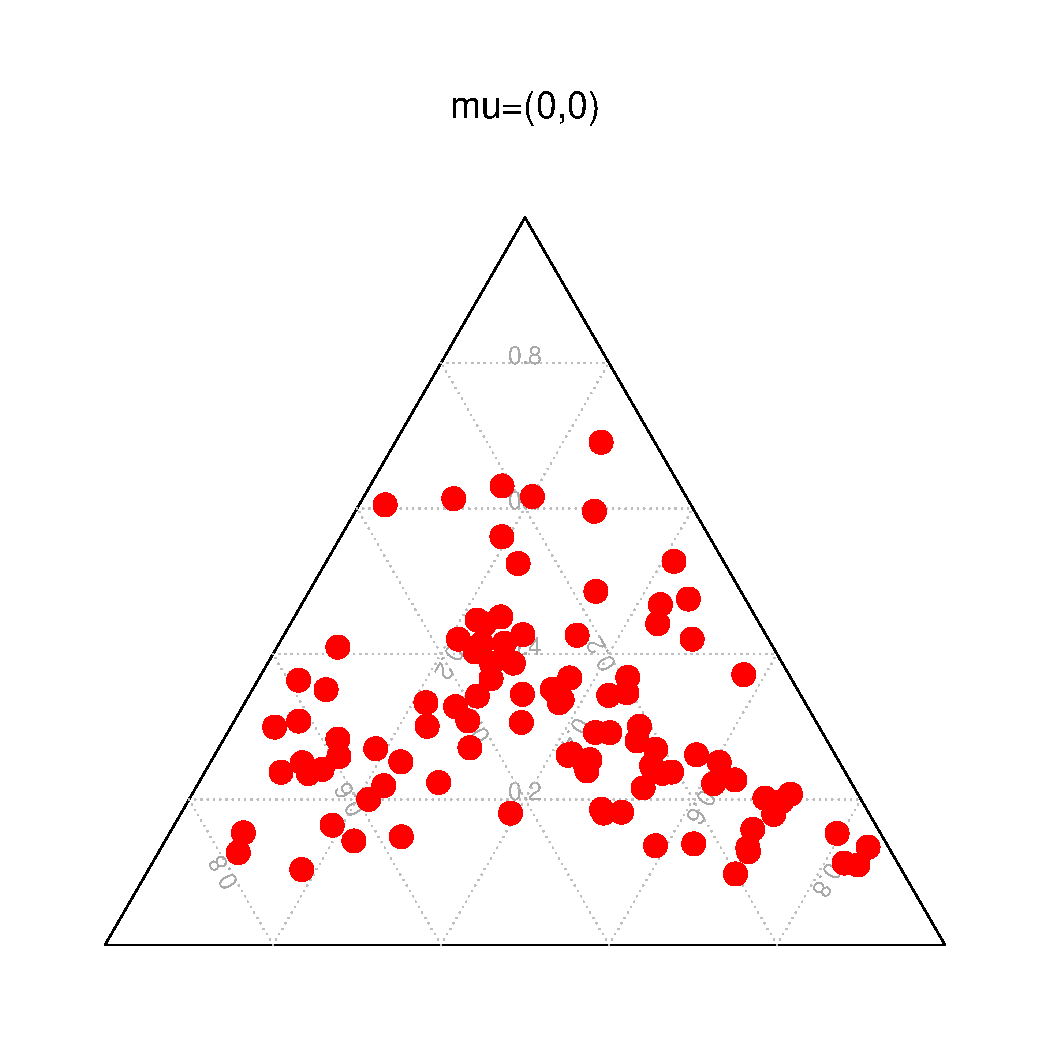
\includegraphics[width=\textwidth]{mu0_0.pdf}
\caption[ALN plot with a zero mean vector]{In this figure, $\muvec$ has all zero entries, with $\Sigma=I$, corresponding to the equiprobable case. Each probability is approximately $1/(d+1)$. }
\label{fig:figure9}
\end{minipage}
\hspace{0.5cm}
\begin{minipage}[b]{0.45\linewidth}
\centering
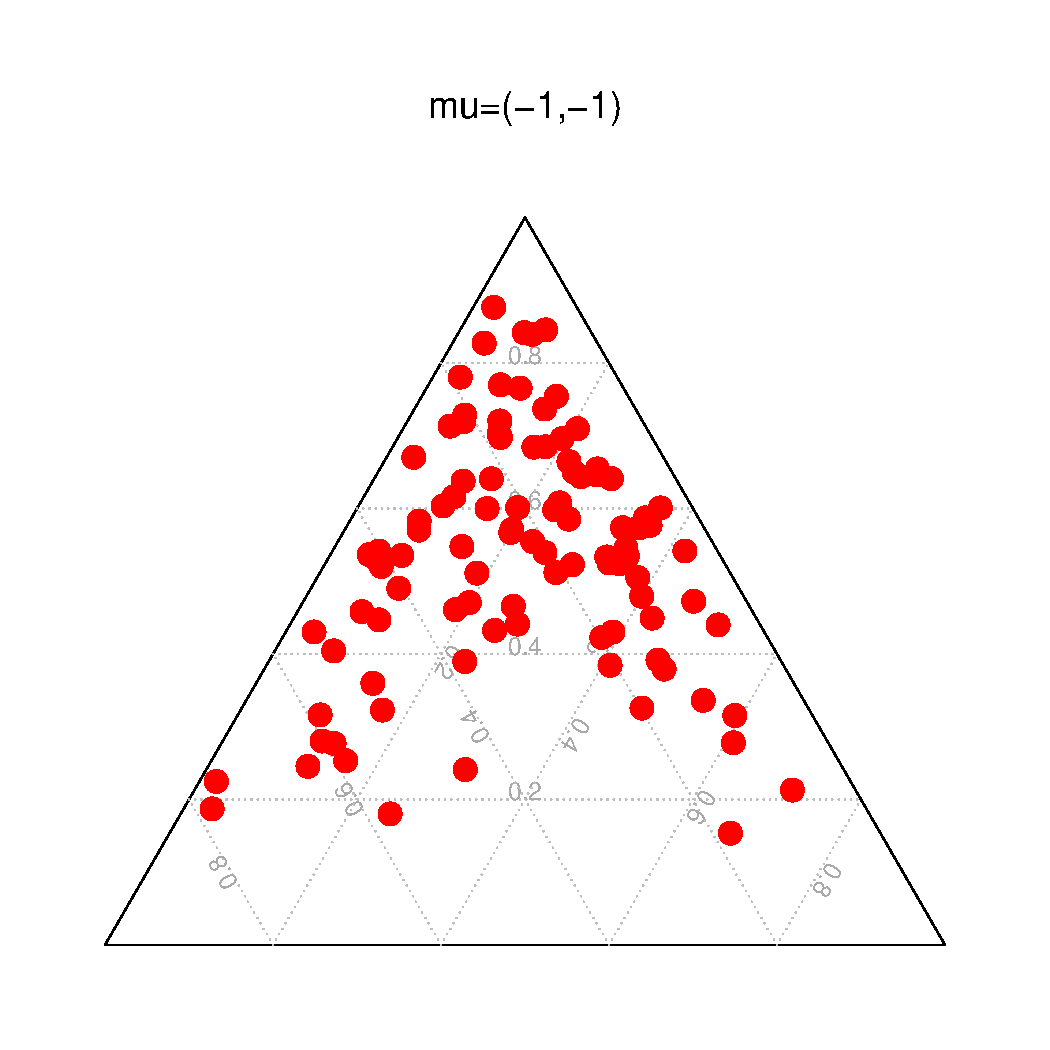
\includegraphics[width=\textwidth]{mu-1-1.pdf}
\caption[ALN plot with a negative one mean vector]{In this figure, $\vec{\mu}=(-1,-1)^T$, with $\Sigma=I$, corresponds to moving towards a sparser set of covariates. }
\label{fig:figure10}
\end{minipage}
\end{figure}

\begin{figure}[ht]
\begin{minipage}[b]{0.45\linewidth}
\centering
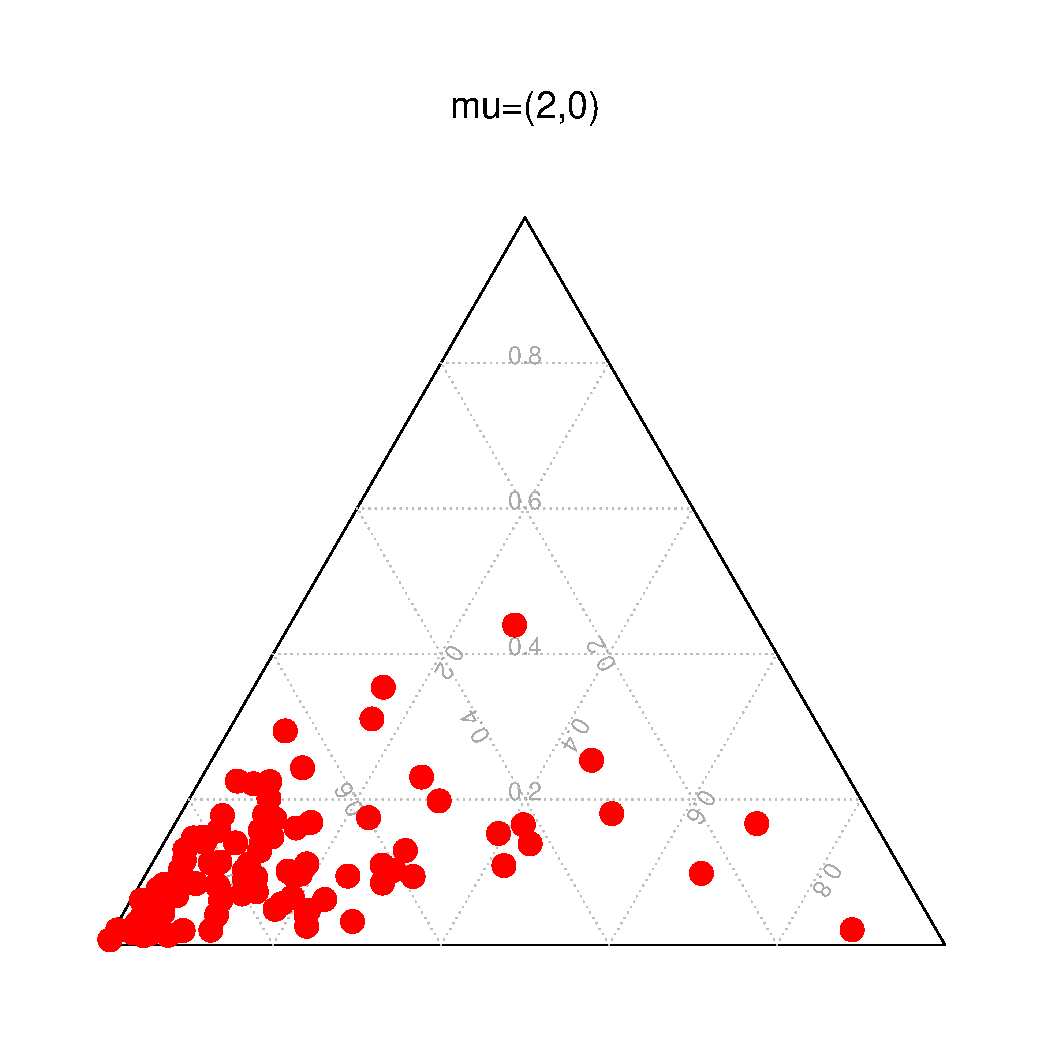
\includegraphics[width=\textwidth]{mu2_0.pdf}
\caption[ALN plot with a mean vector $(2,0)^{T}$]{$\vec{\mu}=(2,0)^T$, with $\Sigma=I$, moves the density towards one corner of the simplex. }
\label{fig:figure1}
\end{minipage}
\hspace{0.5cm}
\begin{minipage}[b]{0.45\linewidth}
\centering
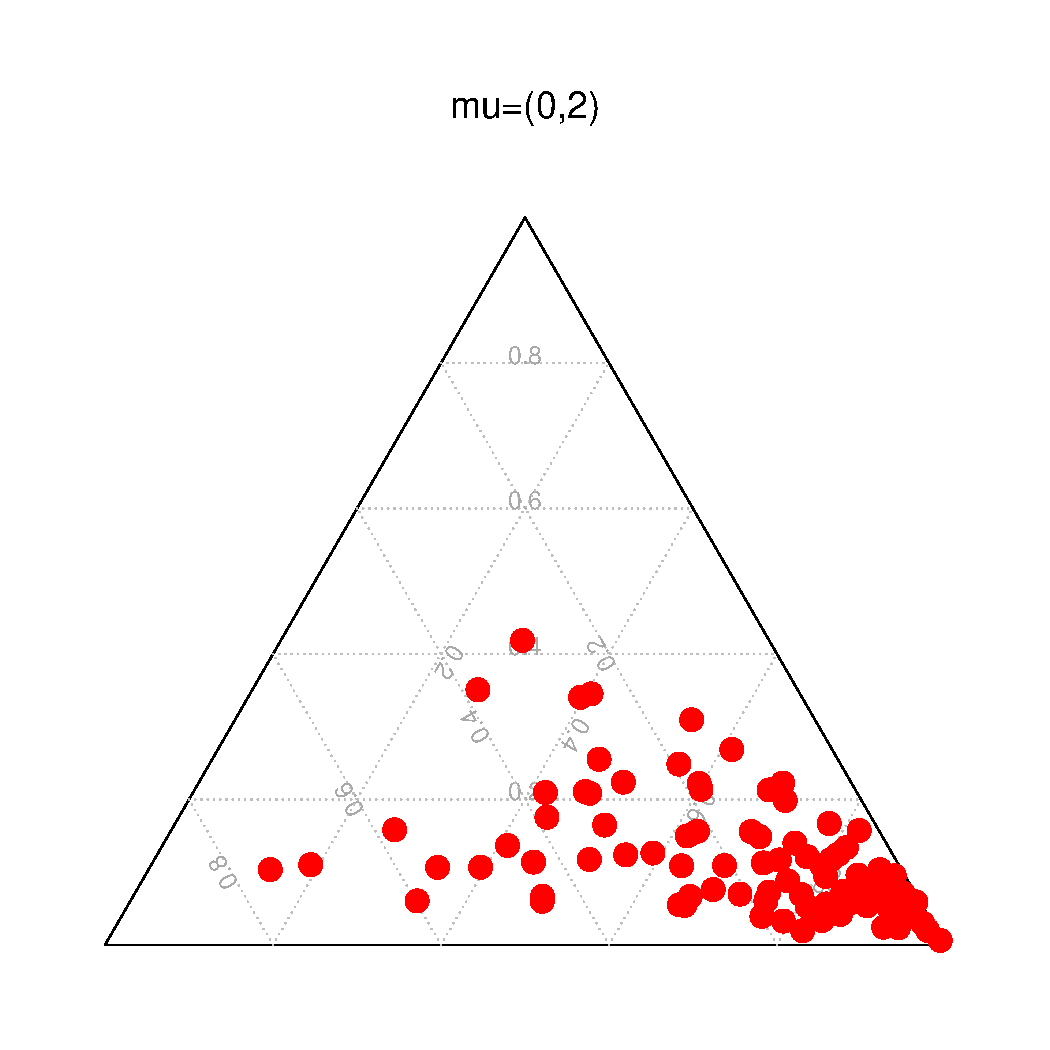
\includegraphics[width=\textwidth]{mu0_2.pdf}
\caption[ALN plot with mean vector $(2,0)^{T}$]{$\vec{\mu}=(0,2)^T$, with $\Sigma=I$, moves the density towards the other corner of the simplex. }
\label{fig:figur2}
\end{minipage}
\end{figure}

\begin{figure}[ht]
\begin{minipage}[b]{0.45\linewidth}
\centering
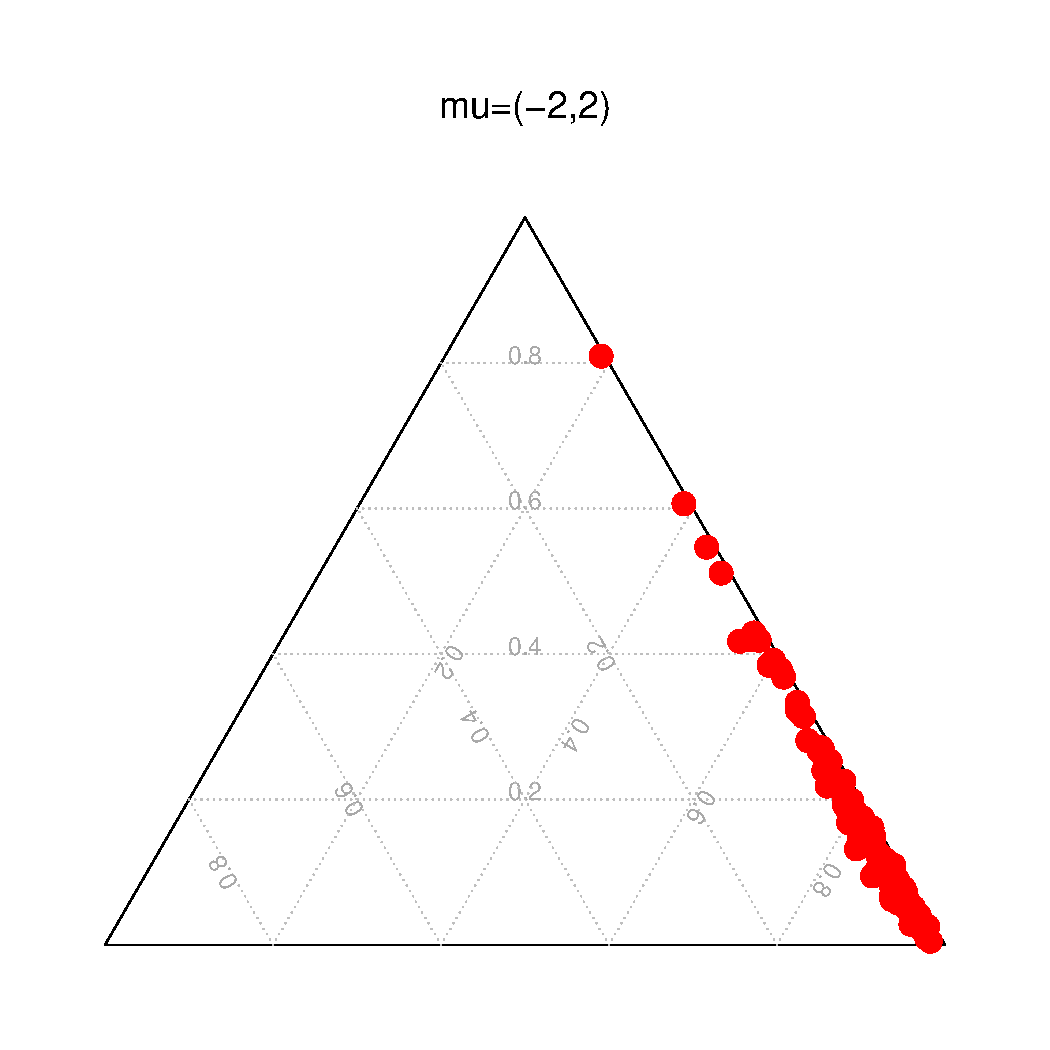
\includegraphics[width=\textwidth]{mu-2_2.pdf}
\caption[ALN plot with a mean vector of $(-2,2)^{T}$]{$\vec{\mu}=(-2,2)^T$, with $\Sigma=I$, corresponds to most probability mass along a corner of the simplex and is a sparse representation.} 
\label{fig:figure3}
\end{minipage}
\hspace{0.5cm}
\begin{minipage}[b]{0.45\linewidth}
\centering
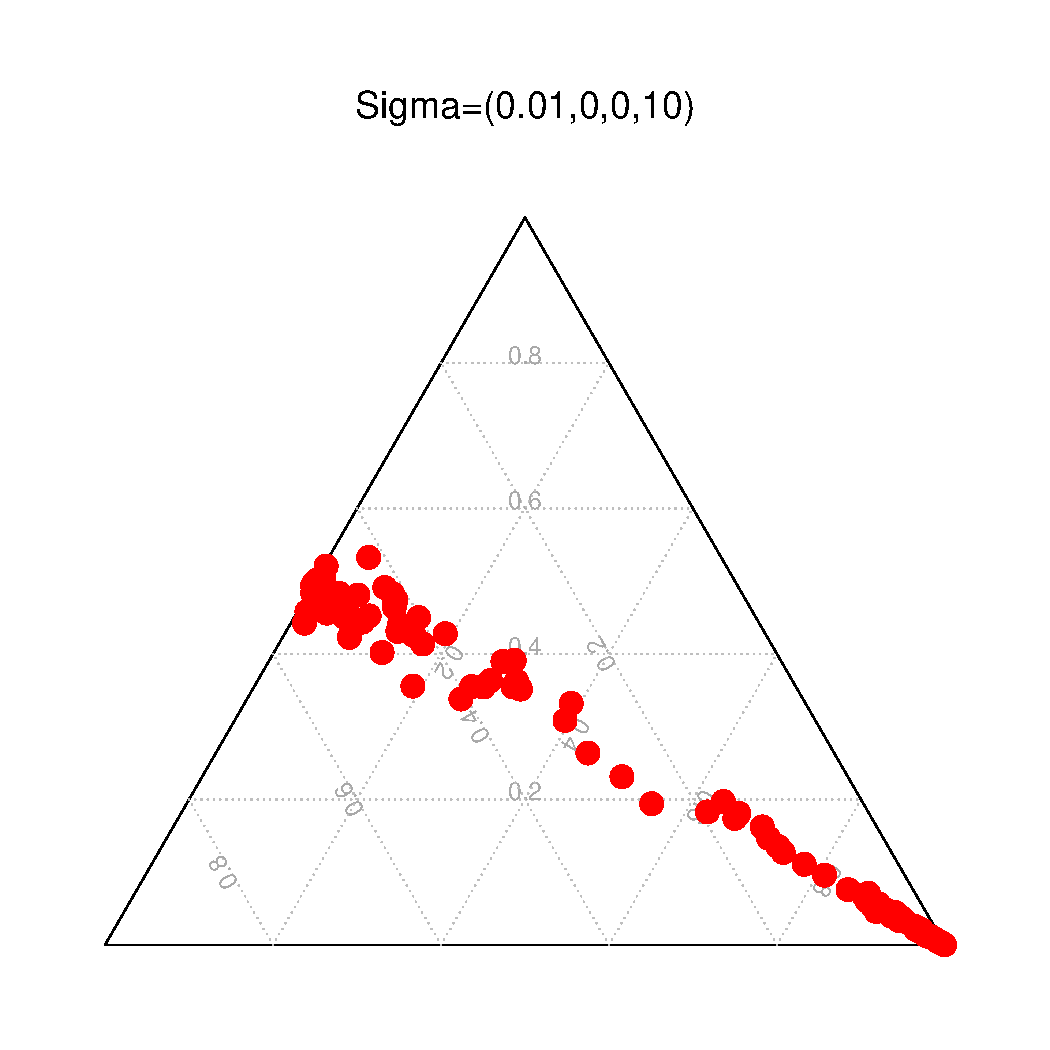
\includegraphics[width=\textwidth]{Sigma0_01_10.pdf}
\caption[ALN plot $\Sigma=\text{Diag(0.01,100)}$]{ $\vec{\mu}=\vec{0}$, with
 $\Sigma= \text{diag}(0.01, 100)$, corresponds to most density lying on a one dimensional subspace (the second covariate in the $\Rsp\ $ space).  }
\label{fig:figure4}
\end{minipage}
\end{figure}


\begin{figure}[ht]
\begin{minipage}[b]{0.45\linewidth}
\centering
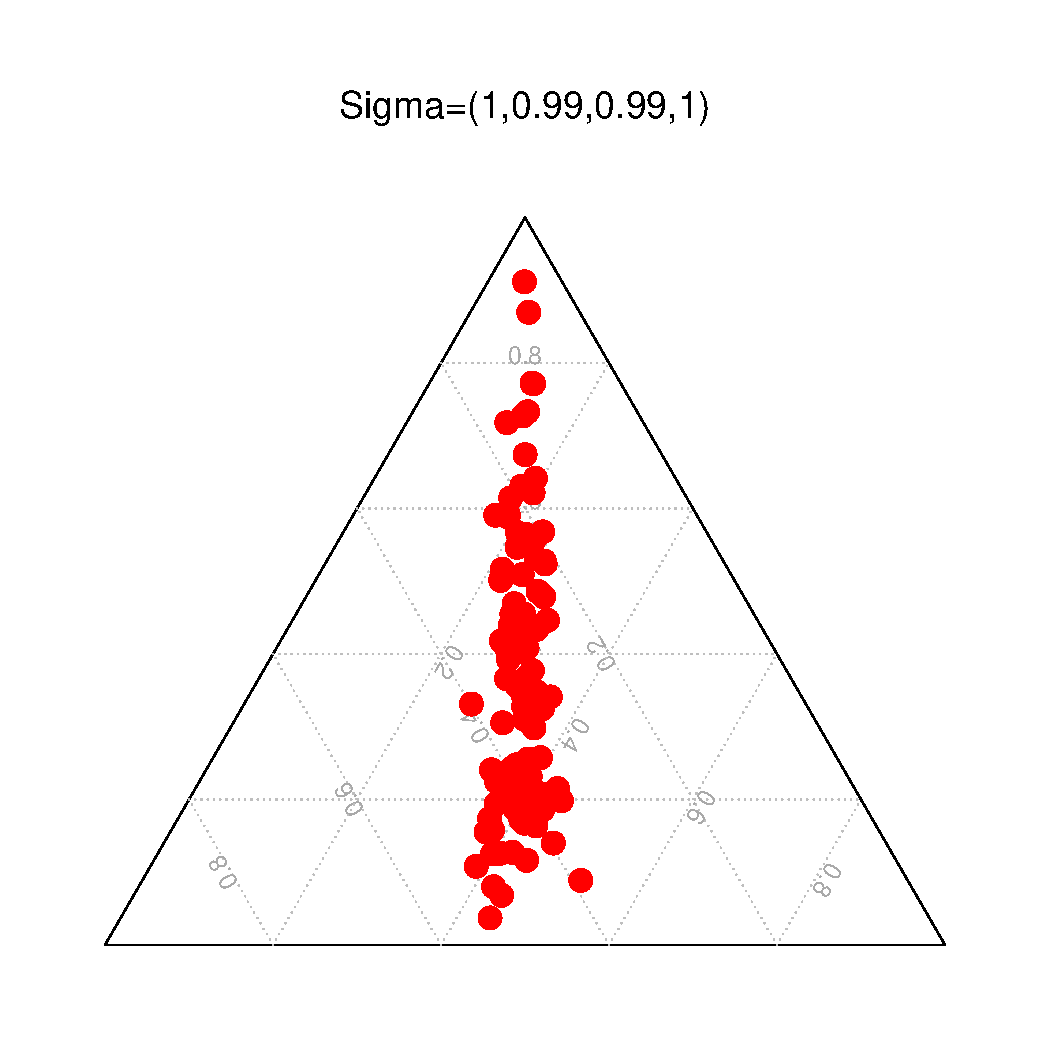
\includegraphics[width=\textwidth]{Sigma1_9_9_1.pdf}
\caption[ALN plot $\Sigma$ numerically singular]{Here $\Sigma$ is approximately singular and most of the probability mass in concentrated along the $d+1$th dimension in the $\mathbb{R}^{d+1}$ space.  }
\label{fig:figure5}
\end{minipage}
\hspace{0.5cm}
\begin{minipage}[b]{0.45\linewidth}
\centering
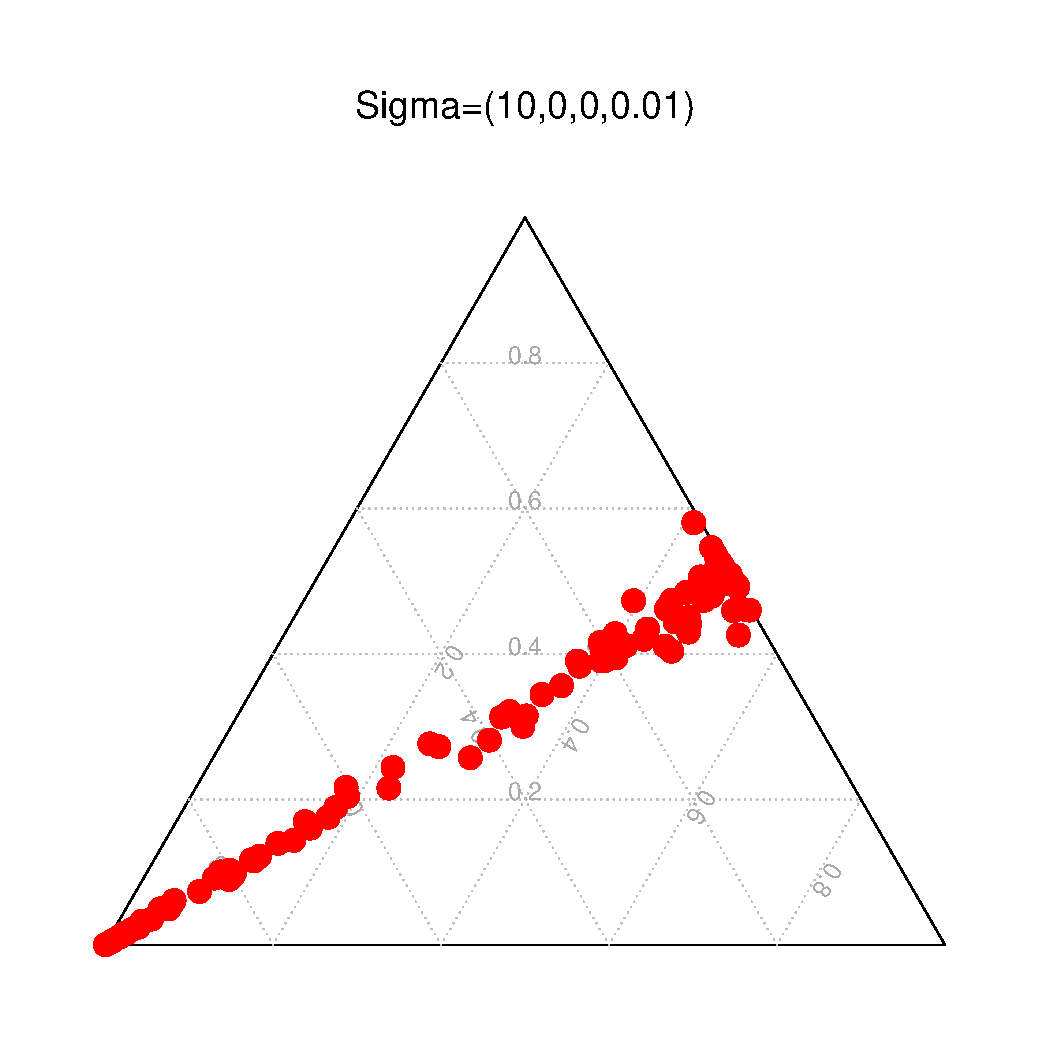
\includegraphics[width=\textwidth]{Sigma10_0_01.pdf}
\caption[Similar to the case in Figure \ref{fig:figure4} but with the variances reversed]{Similar to the case in Figure \ref{fig:figure4} but with the variances reversed.}
\label{fig:figure6}
\end{minipage}
\end{figure}

 \begin{figure}[ht]
\begin{minipage}[b]{0.45\linewidth}
\centering
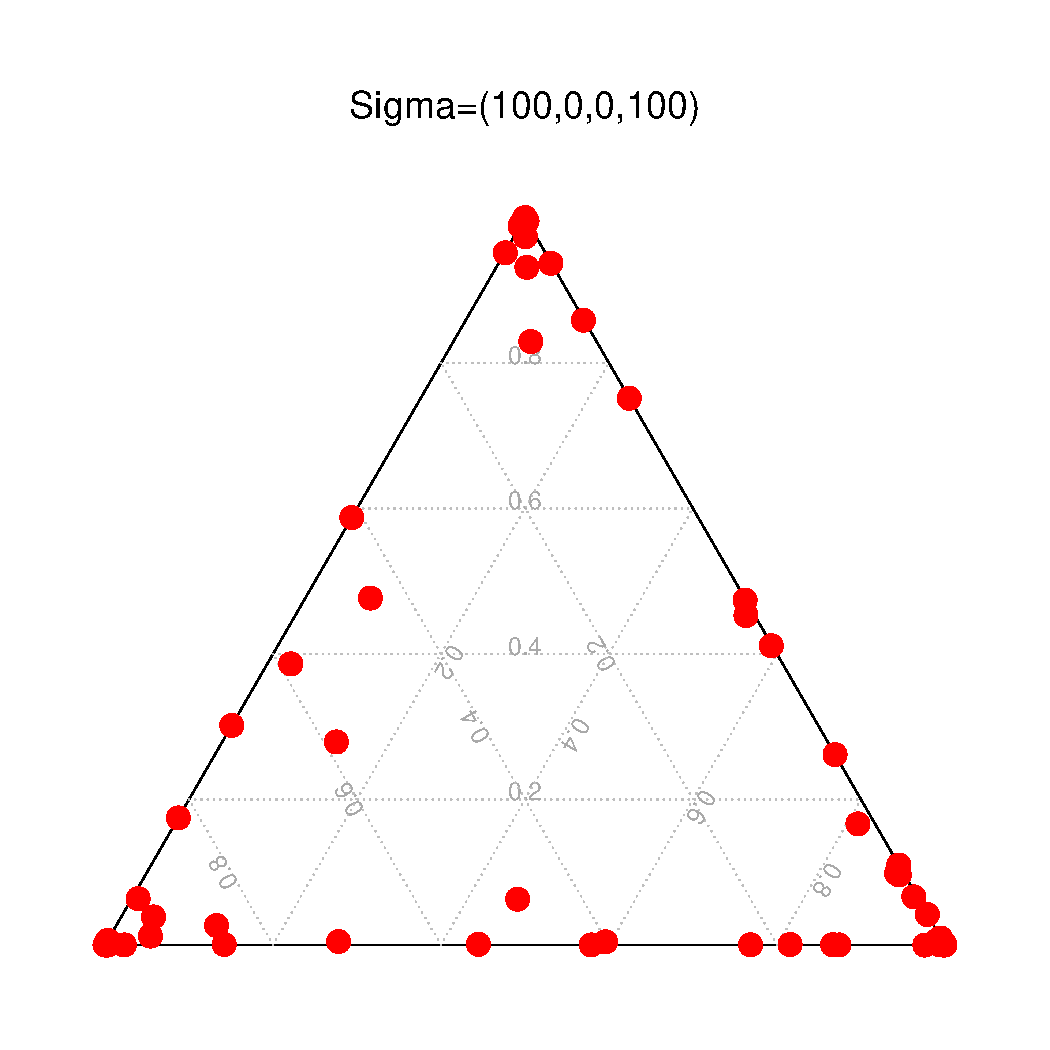
\includegraphics[width=\textwidth]{Sigma100_100.pdf}
\caption[ALN plot with a zero vector mean and $\Sigma=\text{Diag}(100,100)$]{$\vec{\mu}=\vec{0}$, with
 $\Sigma= \text{diag}(100, 100)$, corresponds to encouraging sparse representations \emph{a priori}.  }
\label{fig:figure7}
\end{minipage}
\hspace{0.5cm}
\begin{minipage}[b]{0.45\linewidth}
\centering
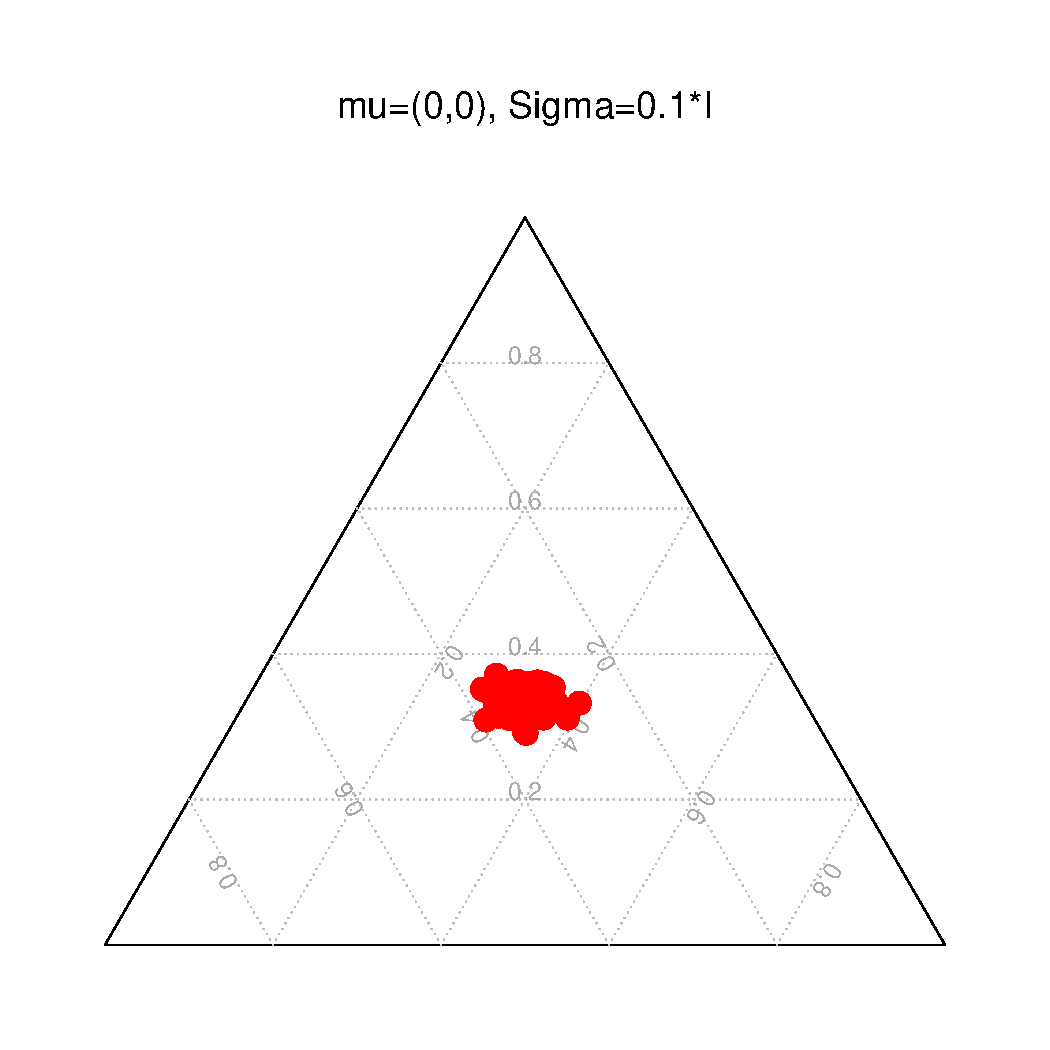
\includegraphics[width=\textwidth]{Sigma01_01.pdf}
\caption[ALN plot approximating the CGM model]{Here $\Sigma=0.1I$, and $\muvec=\vec{0}$, corresponds to roughly the CGM specification.}
\label{fig:figure8}
\end{minipage}
\end{figure}

 The simulations indicate that we can scale everything at approximately an $\mathcal{O}(d)$\newnot{symbol:big_oh} rate because of the diagonality of the variance covariance matrix, no matrix inversions are required. The step that remains is to link this portion of the model with the (currently) observed data in the tree, so that better trees are favored over trees that are worse, when each is observed in the Markov chain. We will first work in the space $\Rsp{d}$ and then translate to probabilities by using Equation \ref{eqn:simplex_transform}.  
 
 If we are to focus on the means and a collection of variances in a multivariate normal i.i.d. model, then we must fully specify the likelihood and the prior to form our posterior. 
 
 The likelihood of the tree is defined as follows: the tree's selected covariates are counted and summed across all observed splits, leading to a likelihood taking on discrete values for the observed data. Let us define a multiplier that can take on an arbitrary positive or negative value in a compact region. We then multiply the counts of splits on each covariate by this quantity, effectively creating a mean which can take on arbitrary values in $\Rsp{}$. 

\subsection{A Simple Sampler Approach}

This subsection derives the full conditional densities for each necessary update in the Gibbs loop to sample posterior weights on each dimension in the CGM decision tree sampler. 
 Throughout this subsection we will use the notation $\odot$\newnot{symbol:hadamard} to denote a Hadamard product of two matrices or vectors. 
 
 \subsubsection{The General Strategy}
 There are many problems with using a Dirichlet prior and a Multinomial conjugate likelihood. The two most glaring problems are the implicit prior assumption of same scales on each covariate and the fact that all covariances or, equivalently, correlations must be negative. If the generative model of the data is a linear model with an interaction term and a decision tree model is fit to the data, then several splits will occur on the two interacting covariates. These splits will occur alternately until the curvature is sufficiently approximated \cite{ishwaran2010high}. This situation indicates a positive correlation between the two covariates. Higher order interactions will result in similar positive correlations between collections of covariates. Therefore we conclude the Dirichlet density as a posterior for the probability of selecting a covariate is an inferior model. Moreover, the initial motivation for modeling data with a decision tree was to handle survey data that contained many complex interactions that would be too computationally expensive to evaluate using linear model methods \cite{morgan1963problems}. 
 
 The likelihood will be denoted by
 
 \begin{equation}\newnot{symbol:mvn}
 MVN(\vec{c}\odot\vec{s}\vert \vec{\mu}, \Sigma=\text{Diag}(\sigma^2_j)).
 \end{equation}
 
 The prior is also a normal 
 
 \begin{equation}
 \pi(\vec{\mu}\vert \vec{\mu}_p, \Sigma)=MVN(\vec{\mu}\vert \vec{\mu}_p, \Sigma).
 \end{equation}

The priors on the variances are \iid $\sim \invgam{\sigma_j^2}{a_j}{b_j}$.
Finally the priors on the $c_j$s are \iid\ scaled beta's with densities 

\begin{equation}\newnot{symbol:scaled_beta}
S\beta(c_j\vert \alpha_j, \beta_j, -a, a)\equiv\pi(c_j\vert \alpha_j, \beta_j, -a, a)= \frac{(c_j+a)^{\alpha_j-1}(a-c_j)^{\beta_j-1}\Gamma(\alpha_j+\beta_j)}{(2a)^{\alpha_j+\beta_j-1}\Gamma(\alpha_j)\Gamma(\beta_j)}.
\end{equation}

A special case of these scaled beta densities is when $\alpha_j=\beta_j=1$, which yields uniform r.v.'s on the region  $[-a,a]$. 
For each $j=1, \dots, d$, we first calculate $s_j = \epsilon+\sum_{\forall \eta \in \mathcal{T}}\mathds{1}[\text{split on covariate j at node $\eta$}]$, for some fixed $\epsilon>0$.
Through basic Bayesian calculations we find that the full conditionals are 

\begin{equation}
\pi(c_j\vert \mu_j, \sigma_j^2, a) \sim N_{[-a,a]}(c_js_j\vert \mu_j, \sigma^2_j) \text{(a normal truncated to the region $(-a,a)$),}
\end{equation}

\begin{equation}
\pi(\sigma^2_j \vert \mu_j, c_j, a) \sim \invgam{\sigma_j^2}{2a_j+2}{\frac{(c_js_j-\mu_j)^2+ (\mu_j-\mu_j^p)^2+b_j}{2}}, \text{ and } 
\end{equation}

\begin{equation}
\pi(\mu_j\vert \mu_j^p, c_j, \sigma^2_j)\sim N[c_js_j+\mu_j^p, \sigma_j^2].
\end{equation}

Ideally we would like everything to be a Gibbs step. This can be accomplished numerically using numerical approximations to the cumulative density of the standard normal distribution, here denoted $\Phi$, and $\Phi^{-1}$, the quantile function of the standard normal cumulative density. \newnot{symbol:sncdf} However, we can accomplish this directly using the technique of parameter expansion set forth in Damien and Walker \cite{damien2001sampling}, which we review here for completeness. 
 
We begin with the joint density of two random variables 

\begin{equation}
f(x,y) \propto \mathds{1}[0, \exp{(-x^2/2)}](y).
\end{equation}
The marginal of $x$ is a standard normal density. Through elementary probability calculations we find 

\begin{equation}\newnot{symbol:unif}
f(y\vert X=x) \propto Unif(0, \exp{(-x^2/2)}).
\end{equation}
 and 
 
 \begin{equation}
f(x\vert Y=y) \propto Unif(-\sqrt{-2log(y)}, \sqrt{-2log(y)})
\end{equation}
 The region upon which $X$ is defined arises from the solution of the inequalities $\{0\leq y \leq \exp{(-x^2/2)} \} $ for $X$, which is a quadratic equation in $X$. Similarly, if we have a truncated distribution truncated to the region $[a,b]$, we write the joint density 
 
 \begin{equation}
 f(x,y)=Unif((0\leq y\leq \exp{(-x^2/2)})\times (a,b)).
 \end{equation}
 Solving the resulting system of inequalities leads to the set 
 
 \begin{equation}
 \{-\sqrt{-2log(y)}, \sqrt{-2log(y)} \} \cap \{a, b\},
 \end{equation}
which results in the region for $x$

\begin{equation}
 \{\text{max}(a,-\sqrt{-2log(y)}), \text{min}(b,\sqrt{-2log(y)} )\} .
 \end{equation}
 Simulating from a truncated normal is equivalent to simulating from two uniforms on the appropriate regions and evaluating a natural logarithm and a square root. 
 
 A special case of these scaled beta densities is when $\alpha_j=\beta_j=1$, which yields uniform random variables on the region $[-a,a]$. 
For each $j=1, \dots, d$, we first calculate $s_j = \epsilon+\sum_{\forall \eta \in \mathcal{T}}\mathds{1}[\text{split on covariate j at node $\eta$}]$, for some fixed $\epsilon>0$.
Through basic Bayesian calculations we find the full conditionals in closed form
 
\begin{equation}\label{eqn:u_given_cjsj}
\pi(u \vert c_js_j, \mu_j, \sigma_j^2)= \text{Unif}(0, \exp{(\frac{-(c_js_j-\mu_j)^2}{2\sigma_j^2} )}),
\end{equation}

\begin{equation}
\pi(c_j \vert u) = \text{Unif}(\text{max}(-a,-\sqrt{-2log(u)}), \text{min}(a,\sqrt{-2log(u)} )),
\end{equation}

\begin{equation}
\pi(\sigma^2_j \vert \mu_j, c_j, a) \sim \invgam{\sigma_j^2}{2a_j+2}{\frac{(c_js_j-\mu_j)^2+ (\mu_j-\mu_j^p)^2+b_j}{2}}, \text{ and}
\end{equation}

\begin{equation}\label{eqn:muj_given_cj}
\pi(\mu_j\vert \mu_j^p, c_j, \sigma^2_j)\sim N[c_js_j+\mu_j^p, \sigma_j^2].
\end{equation}

 The Gibbs sampling step, nested within the MH sampler, proceeds by sampling from Equations \ref{eqn:u_given_cjsj}-\ref{eqn:muj_given_cj}
At each iteration, once samples are drawn in sequence from the distributions given in Equations \ref{eqn:u_given_cjsj}- \ref{eqn:muj_given_cj}, we take the posterior samples of $\mu_j$ and transform these onto the $[0,1]$ scale, by using the ALN transform given in Equation \ref{eqn:simplex_transform}. 

We show results from a preliminary coding of the stated algorithm. We use two specificications for the prior means $\vec{\mu}^p$. One specification uses  $\vec{\mu}^p = \vec{0}$ (Figure \ref{fig:simple_sampler2}) and another uses $\vec{\mu}^p=(-2,-2,2,\dots,2)$ (Figure \ref{fig:simple_sampler1}). The difference in the results of sampled weights indicates that, if we can move from a negative to a positive value for the prior mean, we can greatly influence the selection of covariates. The graphic of posterior weights shown in Figure \ref{fig:simple_sampler1} is the correct set of weights for the data. 


%%%% -------Graphics from preliminary simulations using the simple sampler approach

 \begin{figure}[ht]
\begin{minipage}[b]{0.45\linewidth}
\centering
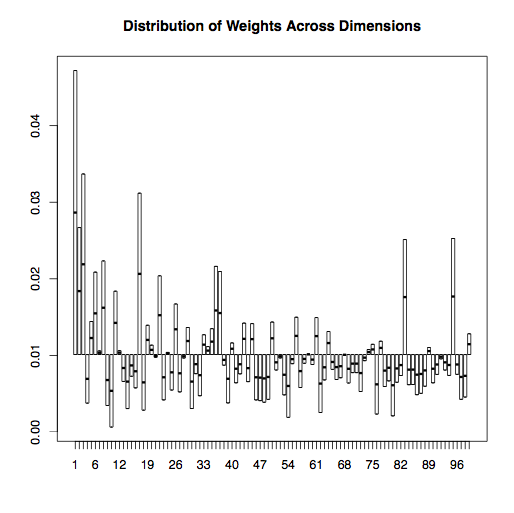
\includegraphics[scale=0.4]{simple_sampler2.png}
\caption[Results for the zero mean prior]{A zero mean prior. Note that the two covariates that should have large probabilities are covariates 1 and 2.}
\label{fig:simple_sampler2}
\end{minipage}
\hspace{0.5cm}
\begin{minipage}[b]{0.45\linewidth}
\centering
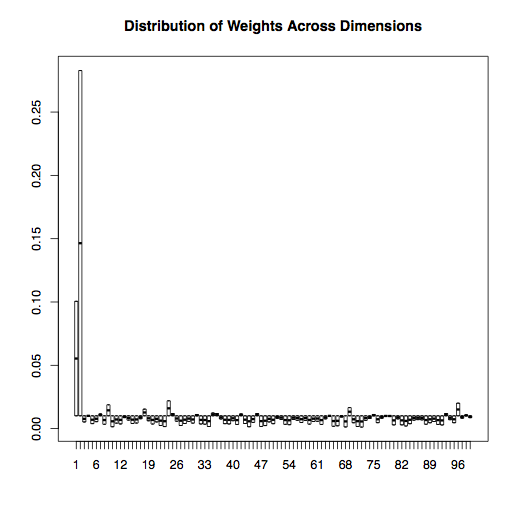
\includegraphics[scale=0.4]{simple_sampler1.png}
\caption[Results for the informative prior]{An informative prior. The first two prior means are 2 and the remaining prior means are set at -2.}
\label{fig:simple_sampler1}
\end{minipage}
\end{figure}


%%%%---------END OF: Graphics from preliminary simulations using the simple sampler approach

\subsection{A Stochastic Search Variable Selection Approach}

Using the results of George and McCulloch we can derive Gibbs updates for each of the parameters and have as a special case the approach of CGM if all the dimension indicators are selected to be the point masses at zero. In this case the ALN transform puts probability $1/(d+1)$ on each dimension. 


We investigate several priors for use in variable selection with decision trees. They are: 

\begin{itemize}
\item A stochastic search approach (method of George and McCulloch and Cui and George) \cite{cui2008empirical,george1993variable}. 
\item A lasso prior on the means of the MVN, \newabbrev{abbrev:MVN} probably using parameter expansion to get Gibbs updates \cite{park2008bayesian}. 
\item A multivariate half-Cauchy prior using parameter expansion (Huang and Wand method) \cite{huang2013simple,polson2011half,carvalho2010horseshoe,carvalhohandling}. 
\item A `local' prior approach (Valen Johnson and David Rossell JRSS B 2010 approach) \cite{johnson2010use}. 
\end{itemize}

We will discuss the preliminary details of each method in sequence in this chapter. 

Variable selection with SSVS facilitates a Bayesian approach to variable selection in decision trees. Prior methods have examined bootstrapping approaches and used some complicated math to allow the statistician to peer inside the black box method known as randomForest \cite{ishwaran2010high, ishwaran2007variable}, often with little insight or understanding. The SSVS prior allows us to ``test'' whether the constant prior probability of selecting a covariate for all dimensions is appropriate for the given dataset. This means we can test, for any dataset, whether the CGM model of covariate selection is appropriate.

We will implement and compare our method against other methods such as observed frequency, a na\"{i}ve method, as well as the maximal subtree approach of Ishwaran et al. \cite{ishwaran2010high, ishwaran2007variable}. The SSVS approach involves a prior on the normal means of the form 

\begin{equation}
\pi(\mu_i\vert \tau_i, p_i, c_i) \propto p_iN(\mu_i, \tau_i^2)+(1-p_i)N(\mu_i, c_i^2\tau_i^2).
\end{equation}

Here the $c_i >1$ and $1>\tau_i>0$ is small. Usually $p_i\equiv1/2$ but it is also possible to put a prior on these hyper-parameters. The advantage of a mixture prior in this form is that Gibbs samples are readily available for each of the desired quantities facilitating fast sampling.     

\subsection{A Lasso Prior}
In this section we propose to use parameter expansion to facilitate Gibbs sampling within the sampling framework for the posterior means for each covariate in the normal space. We use the ALN transform to then convert to probabilities. 
The key idea we use for parameter expansion is the scale mixture of normals representation of a Laplace prior. This representation is stated here for reference.

If $V \sim \text{Exponential(1)}$ and $Z \sim N(0, 1)$ independent of $V$, then $X = \mu + b \sqrt{2 V}Z \sim \mathrm{Laplace}(\mu,b)$. 

Equivalently we can write this as the hierarchy

\begin{equation}\label{eqn:normal_cond_lhood_lasso}
X \vert V \sim N[\mu, \sigma^22V],
\end{equation}

\begin{equation}\newnot{symbol:exponential_dist}
V \sim \text{Exponential}(1), \text{ and}
\end{equation}

\begin{equation}\newnot{symbol:laplace_dist}
X \sim \text{Laplace}(\mu, \sigma)
\end{equation}

What we want to examine here is whether shrinkage along an $L_1$ penalty will achieve similar results to the SSVS approach and give us meaningful results. The belief here is the same as in the SSVS approach, shrinkage will shrink means toward zero in the multivariate normal. These sampled values from the multivariate normal will then be transformed into something on the $[0,1]$ (probability) scale using the ALN transform. Values of zero, or near zero, on the normal space transform into values of approximately $1/(d+1)$. The probabilities with values around $1/(d+1)$ correspond to covariates we are indifferent about. A confounding aspect of interpreting the probabilities is that they must all sum to 1. Therefore if some values are excessively small this may push all the other probabilities to be larger. If something like this happens it is then difficult to determine which covariates are non-informative. Further simulations regarding selecting covariates using the rule of Equation \ref{eqn:cov_inclusion_rule} will be conducted using the ALN transform and will be done on several simulated and real data examples.    

The following result will be useful for parameter expansion. If 

$X\vert a \sim \mathrm{Inv-Gamma}(\nu/2, \nu/a)$ and  $a \sim \mathrm{Inv-Gamma}(1/2,A^2)$, then $\sqrt{X}\sim \mathrm{Half-Cauchy}$. 

\begin{align*}
f(x) &= \int_0^\infty \underbrace{  \frac{\nu^{\nu/2}}{a^{\nu/2}\Gamma(\nu/2)x^{(\nu/2)+1}}\exp{(-\frac{\nu}{ax})}   }_{=f(x\vert a)} \underbrace{\frac{\exp{(-\frac{1}{aA^2})}}{A\sqrt{\pi}a^{3/2}}}_{=f(a)} da\\
&=\frac{\nu^{\nu/2}}{A\sqrt{\pi}\Gamma(\nu/2)x^{(\nu+2)/2}}\underbrace{\int_0^\infty a^{-\nu/2-1/2-1}\exp{(-(1/a)(\nu/x+1/A^2))}da}_{=\text{Inv-Gamma kernel}}\\
&=\frac{\nu^{\nu/2}\Gamma((\nu+1)/2)}{A\sqrt{\pi}\Gamma(\nu/2)x^{(\nu+2)/2}(\nu/x+1/A^2)^{(\nu+1)/2}}\\
&\propto \frac{1}{\sqrt{x}x^{(\nu+1)/2}(\nu/x+1/A^2)^{(\nu+1)/2}}\\
& =\frac{1}{\sqrt{x}(\nu+x/A^2)^{(\nu+1)/2}  }\\
&=\frac{1}{\sqrt{x}(\nu+x/A^2)^{(\nu+1)/2}  }.
\end{align*}

Making the change of variable $x=y^2$, which implies $dx/(2\sqrt{x})=dy$, shows us that 

\begin{equation}
f(y) \propto (1+(y/A)^2/\nu)^{-(\nu+1)/2},
\end{equation}
for $y>0$ which is the definition of a half-Cauchy density. 

Huang and Wand \cite{huang2013simple} indicate that using an inverse-Wishart prior on the variances, with each standard deviation having a half-Cauchy prior, gives a scaled beta marginal for each correlation. At this point it is worth recalling that the t and half-t distributions have as special cases, the Cauchy and half-Cauchy distributions when the degrees of freedom parameter ($\nu$) in the t and half-t is set to $\nu=1$. 



\section{Derivations}
\label{ch:p3sub_theory}

This subsection contains the mathematical details for calculating the integrals to get the closed form solutions for the integrated likelihood equations of the ZIP model described in this chapter.   

%\subsubsection{Normal Derivation}

\subsection{ZIP Derivations}

In this section we provide the derivation for the integrated likelihood for the Bayes ZIP (zero inflated Poisson) tree model. Now let us define our notation, $j$ will index all observations or only the observed zero observations with the upper limit being $n$ or  $n_0$ if the index is all observations or observed zero counts only, respectively.  Also $j^{\prime}$ will exclusively index the non-zero observations. The total number of non-zero observations is denoted $n_+$, so that $n_++n_0=n$, the total number of observations. Finally, let $\bar{y}_{i+}$ denote the sample mean of the non-zero count observations in terminal node $i$. 

The integrated likelihood is:
\begin{align*}
\Pr(Y \vert X, \mathcal{T}) &= \prod_{i=1}^b\int_0^1\int_0^\infty\prod_{j=1}^{n_i}\left[\mathds{1}[y_{ij}=0](\phi+(1-\phi)\exp{(-\lambda)})+\mathds{1}[y_{ij}>0]\frac{\exp{(-\lambda)\lambda^{y_{ij}}}}{y_{ij}!} \right]\pi(\phi_i,\lambda_i )d\lambda_id\phi_i\\
&=\prod_{i=1}^b \int_0^1\int_0^\infty\underbrace{\prod_{j=1}^{n_0}(\phi + (1-\phi)\exp{(-\lambda)})\pi(\phi_i,\lambda_i )d\lambda_id\phi_i}_{=(1)}\\ 
&+ \prod_{i=1}^b \int_0^1\int_0^\infty \underbrace{\prod_{j^\prime=1}^{n_+}\frac{\exp{(-\lambda)}\lambda^{y_{ij^\prime}} }{y_{ij^\prime}!}\pi(\phi_i,\lambda_i )d\lambda_id\phi_i}_{=(2)}.\\ 
\end{align*} 
We will first tackle $(1)$, then $(2)$. 

\begin{align*}
(1)&= \int_0^1\int_0^\infty\prod_{j=1}^{n_0}(\phi + (1-\phi)\exp{(-\lambda)})\pi(\phi_i,\lambda_i )d\lambda_id\phi_i \\
&= \int_0^1\int_0^\infty(\phi + (1-\phi)\exp{(-\lambda)})^{n_0}\pi(\phi_i,\lambda_i )d\lambda_id\phi_i \\
&= \int_0^1\int_0^\infty\sum_{j=1}^{n_0}{n_0\choose j}\phi^{j}(1-\phi)^{n_0-j}\exp{(-(n_0-j)\lambda)})\pi(\phi_i)\pi(\lambda_i )d\lambda_id\phi_i. \\
\end{align*}
Now, we take $\pi(\phi_i)$ to be a beta($\alpha, \beta$) prior and $\pi(\lambda_i)$ to be a gamma($\alpha_{\lambda}, \beta_{\lambda}$) prior. This simplifies matters greatly. The last equation above with a double integral becomes:
 \begin{align*}
 & \int_0^1\int_0^\infty\sum_{j=1}^{n_0}{n_0\choose j}\phi^{j}(1-\phi)^{n_0-j}\exp{(-(n_0-j)\lambda)})\frac{\Gamma(\alpha+\beta)\phi^{\alpha-1}(1-\phi)^{\beta-1}}{\Gamma(\alpha)\Gamma(\beta)}\frac{\lambda^{\alpha_{\lambda}-1}\exp{(-\lambda/\beta_{\lambda})}}{\Gamma(\alpha_{\lambda})\beta_{\lambda}^{\alpha_{\lambda}}} d\lambda_id\phi_i \\
&=\sum_{j=1}^{n_0}{n_0\choose j}\frac{\Gamma(\alpha+\beta)}{\Gamma(\alpha)\Gamma(\beta)\Gamma(\alpha_{\lambda})\beta_{\lambda}^{\alpha_{\lambda}}} \underbrace{\int_0^1\phi^{j+\alpha-1}(1-\phi)^{\beta+n_0-j-1}d\phi_i}_{\text{a beta kernel}}  \underbrace{\int_0^\infty \lambda^{\alpha_{\lambda}-1} \exp{(-(n_0-j+\beta_{\lambda}^{-1})\lambda)} d\lambda_i}_{\text{a gamma kernel}}\\
&=\underbrace{\sum_{j=1}^{n_0}{n_0\choose j}\frac{\Gamma(\alpha+\beta)}{\Gamma(\alpha)\Gamma(\beta)\Gamma(\alpha_{\lambda})\beta_{\lambda}^{\alpha_{\lambda}}} \frac{\Gamma(\alpha+j)\Gamma(\beta+n_0-j)\Gamma(\alpha_{\lambda})}{\Gamma(\alpha+\beta+n_0)}(n_0-j+\beta_{\lambda}^{-1})^{\alpha_{\lambda}}}_{=(1)}.
\end{align*} 
Now with the first piece simplified, we move on to piece $(2)$. 
 
 \begin{align*}
 (2) &= \int_0^1\int_0^\infty\prod_{j^\prime=1}^{n_+}\frac{\exp{(-\lambda)}\lambda^{y_{ij^\prime}} }{y_{ij^\prime}!}\pi(\phi_i,\lambda_i )d\lambda_id\phi_i \\
 &= \int_0^\infty \prod_{j^\prime=1}^{n_+}\frac{\exp{(-\lambda)}\lambda^{y_{ij^\prime}} }{y_{ij^\prime}!}\pi(\lambda_i )d\lambda_i \\
 &= \int_0^\infty\frac{\exp{(-n_+\lambda)}\lambda^{n_+\bar{y}_{i+}} }{\prod_{j^\prime=1}^{n_+}y_{ij^\prime}!}\pi(\lambda_i )d\lambda_i \\
 &= \int_0^\infty\frac{\exp{(-n_+\lambda)}\lambda^{n_+\bar{y}_{i+}} }{\prod_{j^\prime=1}^{n_+}y_{ij^\prime}!}\frac{\lambda^{\alpha_{\lambda}-1}\exp{(-\lambda/\beta_{\lambda})}}{\Gamma(\alpha_{\lambda})}d\lambda_i \\
 &= \frac{\int_0^\infty\exp{(-(n_+ +\beta_{\lambda}^{-1})\lambda)}\lambda^{n_+\bar{y}_{i+} +\alpha_{\lambda}-1} d\lambda_i}{\Gamma(\alpha_{\lambda})\prod_{j^\prime=1}^{n_+}y_{ij^\prime}!} \\
 &= \underbrace{\frac{\Gamma(n_+\bar{y}_{i+}+\alpha_{\lambda})(n_+ +\beta_{\lambda}^{-1})^{n_+\bar{y}_{i+}+\alpha_{\lambda}}}{\Gamma(\alpha_{\lambda})\prod_{j^\prime=1}^{n_+}y_{ij^\prime}!}}_{=(2)}. \\
 \end{align*}
This is all the result we need putting the two parts together now gives the closed form for the integrated likelihood. We rewrite Equation \ref{eqn:zip_int_lhood} here for completeness, 

\begin{align}\nonumber
 \Pr(Y\vert X, \mathcal{T})& = \left[\sum_{j=0}^{n_0} {n_0 \choose j}\frac{\Gamma(\alpha+\beta)\Gamma(\alpha+j)\Gamma(n_0+\beta-j)}{\Gamma(\alpha)\Gamma(\beta)\Gamma(\alpha+\beta+n_0)}\left(\frac{n_0-j+\beta_{\lambda}^{-1}}{\beta_{\lambda}}\right)^{\alpha_{\lambda}} \right] \\ \nonumber
 & + \frac{\Gamma(\alpha_{\lambda}+n_+\bar{y}_+)}{\Gamma(\alpha_{\lambda})\beta_{\lambda}^{\alpha_{\lambda}}}\left(n_+ + 1/\beta_{\lambda} \right)^{\alpha_{\lambda}+n_+\bar{y}_+}.
\end{align}

\newpage

\chapter{Bayesian Decision Tree Models}\label{sec:Model}

In Sections \ref{sec:lhood} and \ref{subsec:alt} we describe how we use the ALT to link sparse linear models with covariate selection probabilities facilitating sparse Bayesian decision trees. In Section \ref{subsec:the_tp} we describe the tree prior and the local updates we use to explore the graph of permissible trees. Finally, in Section \ref{subsec:Regularization Priors} we give several examples of regularization priors we will study in our simulated examples.

	\section{The Likelihood}\label{sec:lhood}

We begin by reviewing the model proposed in Chipman et al. \cite{chipman1998bayesian}, and show how our approaches generalize upon their model. 

The response data is usually assumed to be observed from a normal or multinomial likelihood function. Nonetheless, other forms of response data such as zero inflated models are possible \cite{Roberts:2014fk}. The likelihood is denoted 

\begin{equation}\label{eqn:cgm_likelihood}
\mathcal{L}(\mathcal{T}, \vec{q}, \vec{\theta} \vert \vec{y} X)=\Pr(\vec{y} \vert X, \mathcal{T}, \vec{q}, \vec{\theta}).
\end{equation} 
		
\noindent Here the $\vec{y}$ denotes the vector of responses, $X$ denotes the matrix of covariates, and $\mathcal{T}$ denotes the tree. The vector $\vec{q}$ is the vector of covariate selection probabilities and $\vec{\theta}$ denotes the vector of parameters in the terminal nodes of the tree. The parameters that we are interested in are: $\mathcal{T}$, $\vec{\theta}$, and $\vec{q}$. We factorize the prior in a similar fashion to Chipman et al. using the breakdown 

\begin{equation}\label{eqn:prior}
\Pr(\mathcal{T}, \vec{q}, \vec{\theta}) \propto \Pr(\vec{\theta} \vert \mathcal{T}) \Pr(\vec{q} \vert \mathcal{T})\Pr(\mathcal{T}).
\end{equation} 

The framework in Chipman et al. \cite{chipman1998bayesian} proposed assumed $\vec{q} \propto 1/p$. Although we find this prior to be a strong \emph{a priori} assumption to take with a large dimensional covariate space, this prior will be seen as a special case of the SSVS prior presented in Section \ref{sec:ALoVaS_model}. Practical difficulties with the uniform prior were already noted in the discussion of Chipman et al. \cite{knight1998bayesian}, although, little work has been done in the interim to remedy this drawback. We modify the framework of Chipman et al. to allow the $\vec{q}$ to vary, depending on their relevance. We specify a prior on the $\mu_j$, a linear space, and use the \ALT\ to determine (indirectly) the prior on the probability space of the $\vec{q}$. This prior specification on the $\mu_j$ allows one to use the methods of the sparse linear model literature but instead apply these methods to decision trees. 

The prior density for $\vec{q}$, the covariate selection probabilities, is defined in Subsection \ref{subsec:alt}. Similar to Chipman et al., we place the uniform prior, denoted $\Pr(\mathcal{T})$, on the decision tree space. We sample the decision trees using the stochastic process defined in Section \ref{subsec:the_tp}.  To monitor the convergence of the Markov chain used to sample the space of decision trees, it is necessary to be able to calculate the marginal density for $\mathcal{T}$ given the covariate selection probabilities $\vec{q}$. This requires choosing conjugate priors for the vector $\vec{\theta}$ so that a closed form marginal density, $\Pr(\vec{y}\vert X,\vec{q},\mathcal{T})$ is available. Thus, if the response data are continuous, we choose a Gaussian density for the prior on $\vec{\theta}$. Similarly, if the response data are categorical, we choose a Dirichlet density as the prior density for $\vec{\theta}$.  

	\section{The Additive Logistic Transform}\label{subsec:alt}
	
	The ALT, defined in Equation \ref{eqn:alt}, is a mapping from a Euclidean space to a probability space. 
	%We define our model on a Euclidean space and then, once the draw from the posterior is simulated, we transform the draw to a probability scale using the ALT. 
	The ALT was proposed previously as a fundamental transform for use in compositional data analysis \cite{aitchison1986statistical}. 
	
	The additive logistic normal (ALN) density is obtained as a result of transforming a multivariate normal density using the ALT. The ALN density is given in Equation \ref{eqn:aln}, however we will rarely find use for this equation. Rather, the density on $\vec{\mu}$ is a multivariate normal density with a linear scale. When a probability scale is needed, we apply the ALT to the normal random variates, $\vec{\mu}$, to obtain probabilities. 	
\begin{equation}\label{eqn:aln}
f(\vec{q}\vert \mu, \Sigma) = \left[(2\pi)^p\vert\Sigma\vert\left(\prod_{j=1}^{p}q_j\right)^2\right]^{-1/2}\exp\left[ -\frac{1}{2}(log(\vec{q}_{(p)}/q_{p}) - \vec{\mu})^T \Sigma^{-1}(log(\vec{q}_{(p)}/q_{p}) - \vec{\mu}) \right].
\end{equation} 
In Equation \ref{eqn:aln} the notation $\vec{q}_{(p)}$ indicates a vector with the $p$th entry removed. This density is the result of applying the transformation $q_j = \frac{e^{\mu_j}}{1+\sum_{i=1}^{p-1}e^{\mu_i}}$, for $i=1,\dots,p-1$, and the $p$-dimensional vector, $\vec{\mu}$, has a multivariate normal density with mean vector $\vec{\mu}^\prime$ and covariance matrix $\Sigma$. 
The ALN distribution is defined on the $p-1$ dimensional simplex so that $\sum_{j=1}^{p}q_j =1$. Various settings of the parameters $\vec{\mu}^\prime$ and $\Sigma$ correspond to probabilities concentrated on different regions of the $p-1$ simplex. In practice we do not make use of Equation \ref{eqn:aln}, instead we sample from multivariate normals and transform our random variables using the \ALT. Thus the transformed sampled variates, now representing covariate selection probabilities, have a density defined by Equation \ref{eqn:aln}. To help the reader gain intuition into this distribution, we generate plots for the cases where $\vec{q}$ is a $3$-dimensional vector. The simplex plots illustrate the effect of changes in the multivariate normal parameters on the density in the simplex space. 

In Figure \ref{fig:aln_plots}, the four sub-figures represent sampled observations from a normal distribution after applying the ALT. The extreme points in the simplex correspond to sparse covariate selection probabilities and therefore result in sparse decision trees. In (c), we see data concentrated mostly around the point of the simplex $(1/3,1/3,1/3)$, corresponding to independent standard normals. In sub-figure (d), we see the effect of increasing the variance of the normal densities while maintaining zero means. The larger variances make the draws more likely to come from regions near the edge of the simplex.  In sub-figure (e), we see the effect of adding correlation to the multivariate normal density while keeping the mean vector equal to zero. In this parametrization the density lies close to a plane and after transformation to the simplex space the density is concentrated around a line. In sub-figure (f), we see the result of shifting the mean from the zero to the point $(-2,2,0)$. In our simulation studies the parameter changes will be less pronounced and less isolated. Often we will have the four types of changes presented in these images occurring simultaneously. 

\begin{figure}
\begin{center} 
\begin{tabular}{cc}
  \subfigure[]{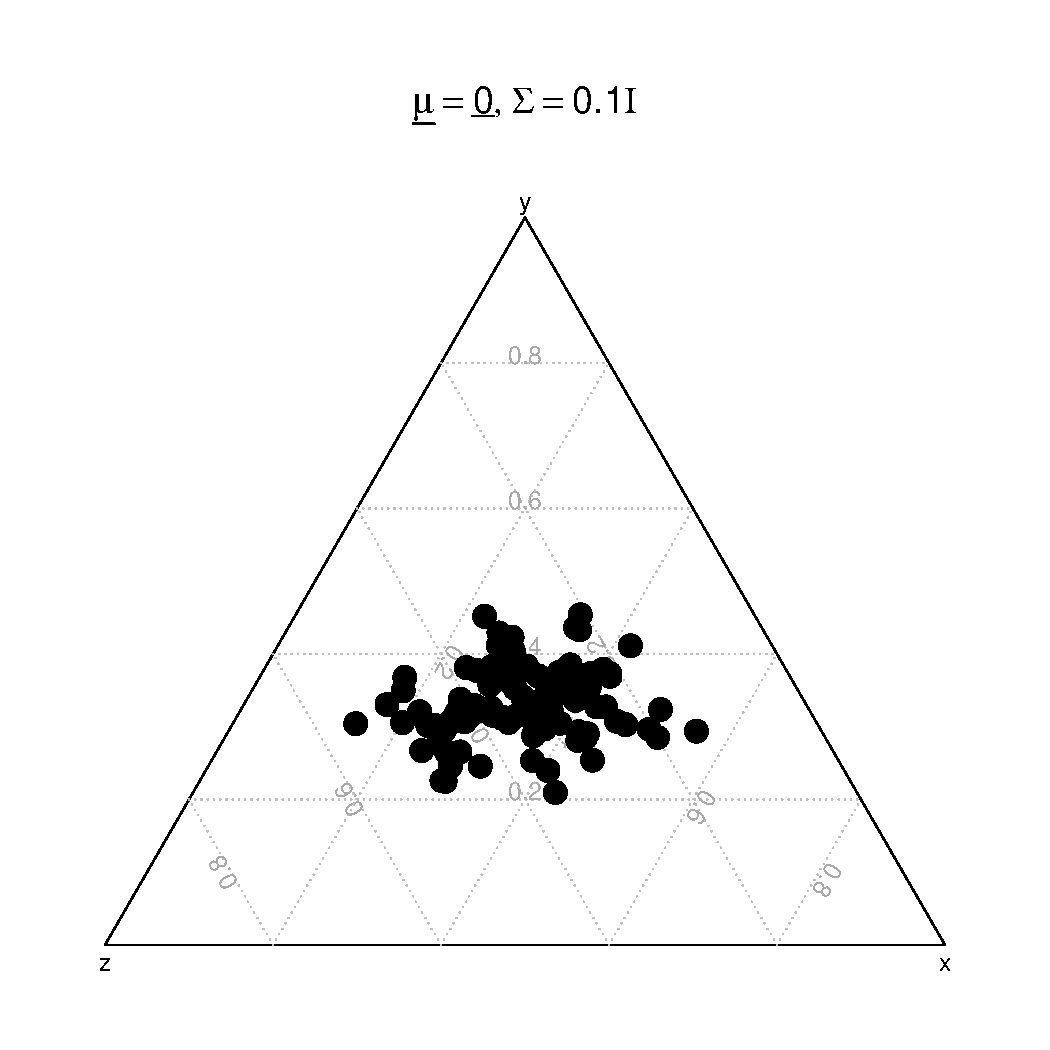
\includegraphics[scale=0.25]{figures/mu0_0_bw.pdf}}
    & \subfigure[]{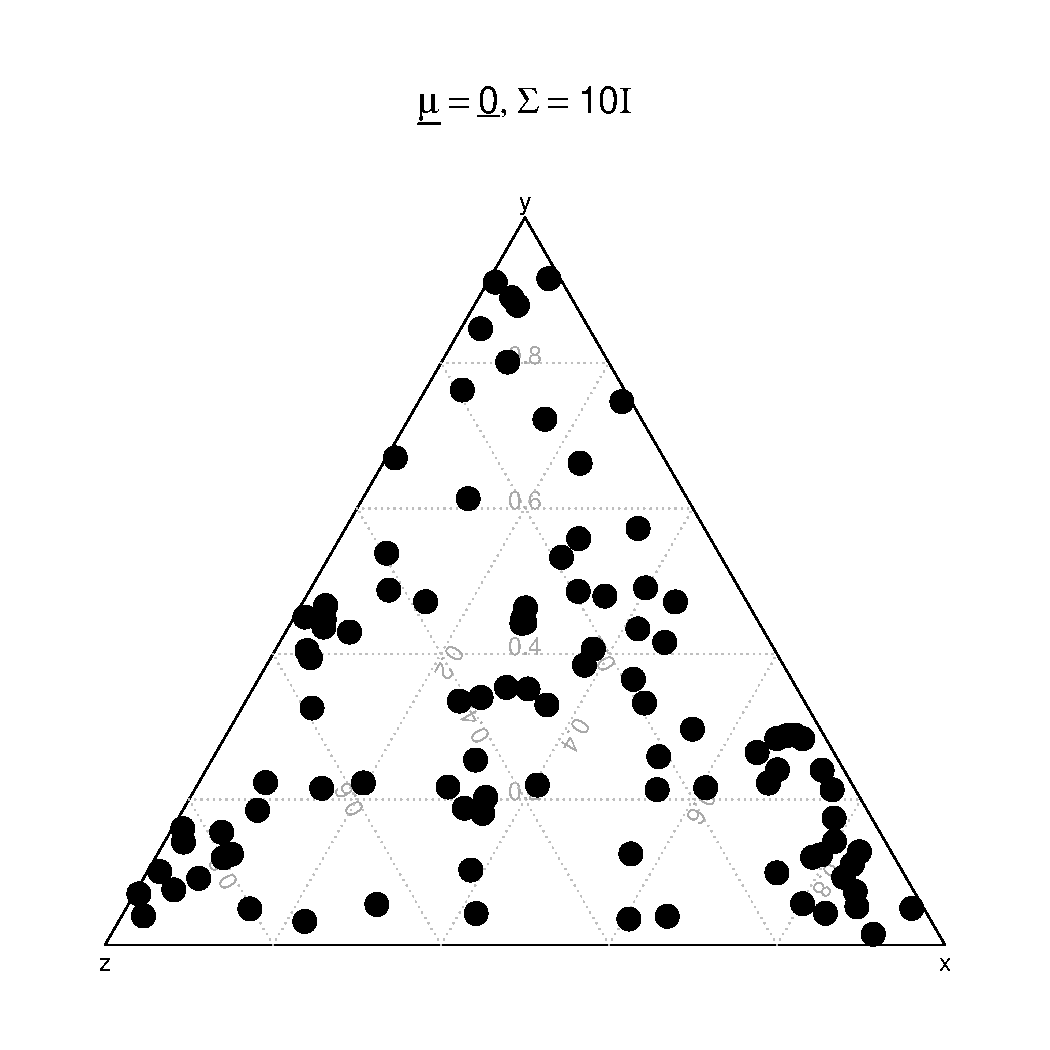
\includegraphics[scale=0.25]{figures/sigma3_3_bw.pdf}} \\
  \subfigure[]{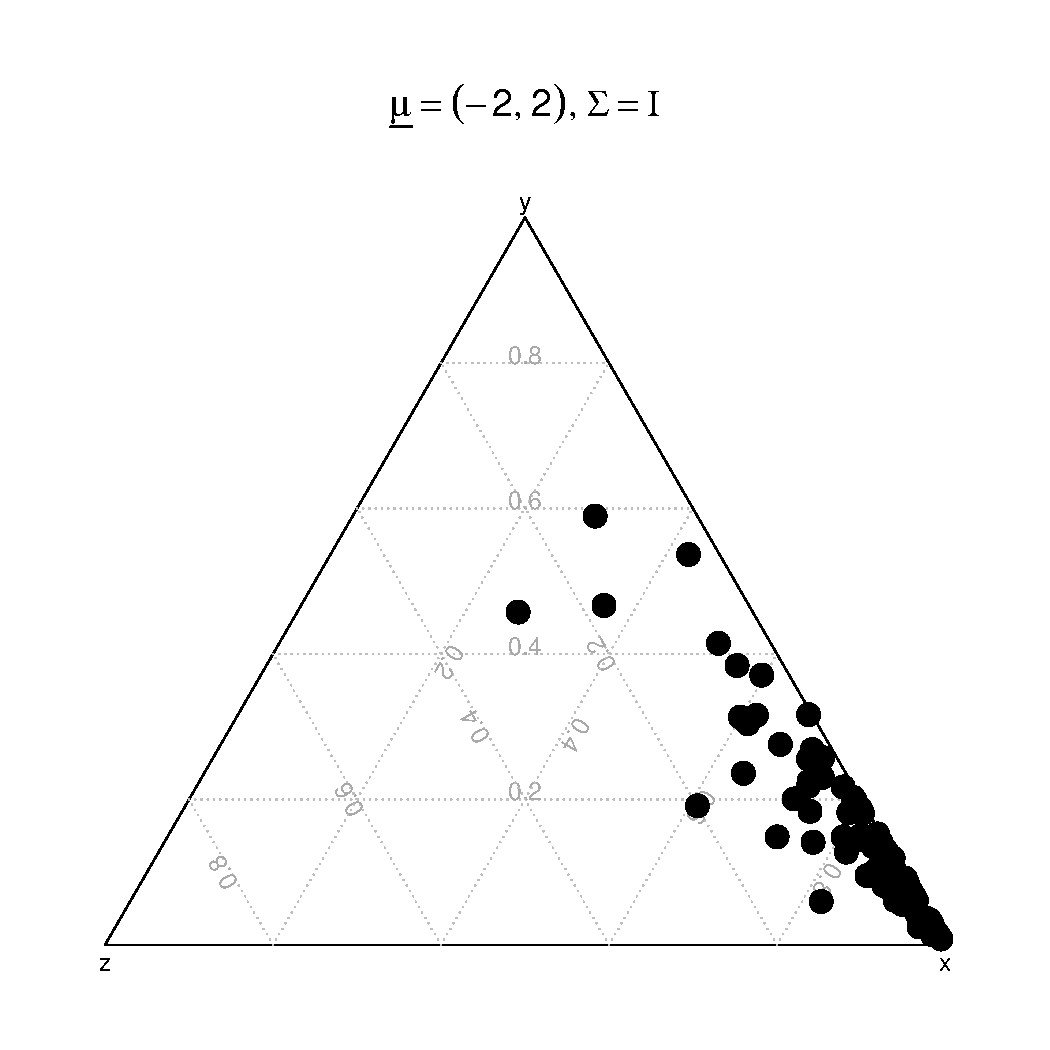
\includegraphics[scale=0.25]{figures/mu2_0_bw.pdf}}
    & \subfigure[]{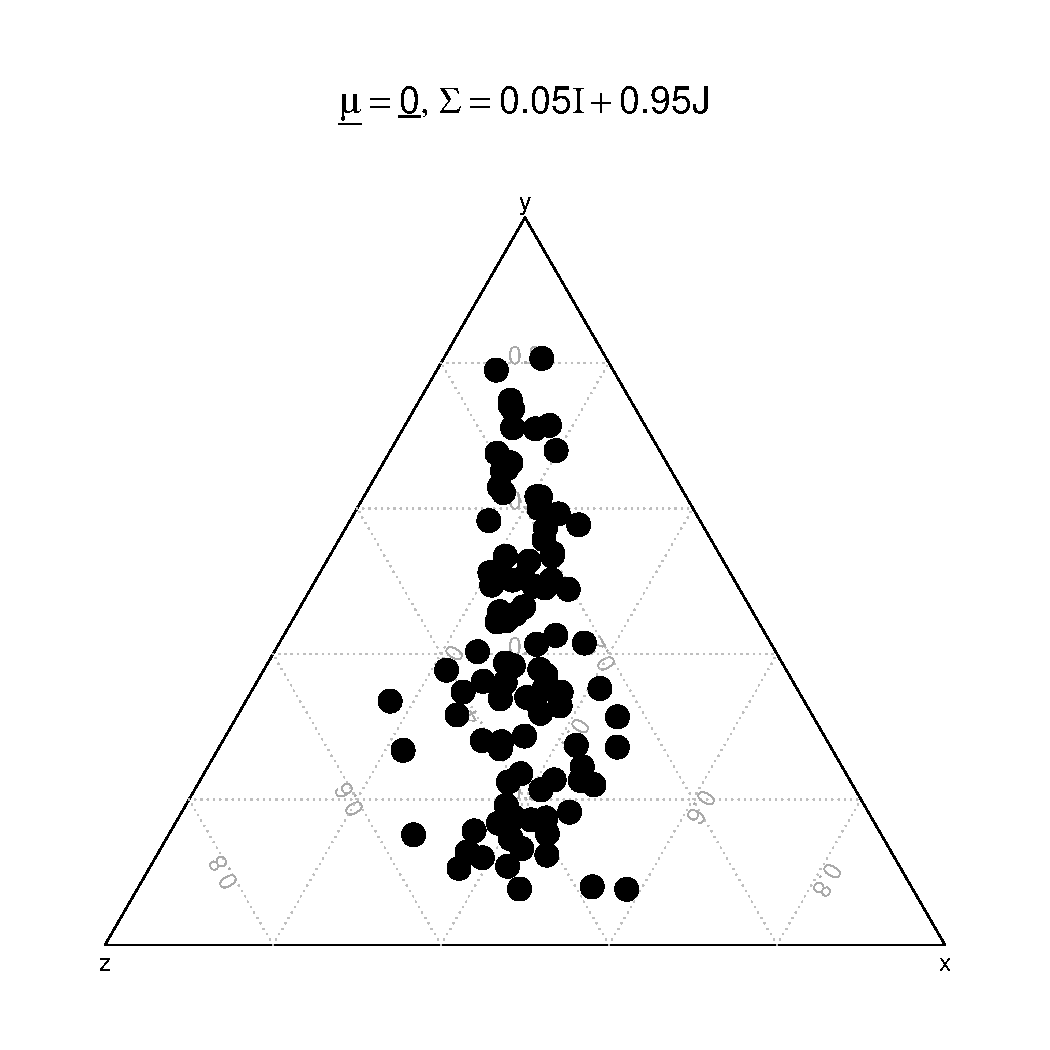
\includegraphics[scale=0.25]{figures/sigma1_9_9_1_bw.pdf}} \\
\end{tabular}
\caption{ALN plots with various multivariate normal parameters. Subfigure (a) contains multivariate standard normal draws. Subfigure (b) plots multivariate normal draws with zero mean and large independent variances. In subfigure (c), contains unit independent variances with mean vector $\mu = (-2,2,0)$. Finally, in subfigure (d) we add correlations while keeping the mean vector as a zero vector. }
\label{fig:aln_plots}
\end{center}
\end{figure}

\section{The Tree Prior}\label{subsec:the_tp}	
This section reviews the tree prior first described in Chipman et al. \cite{chipman1998bayesian}, for those readers that are not familiar with the model. Those readers familiar with the paper may safely skip this subsection. 

The tree prior is defined as

\begin{equation} \label{eqn:tree_prior}
\Pr(\mathcal{T}\vert \vec{q}) = \prod_{\eta\in N} \Pr{_{\text{split}}} (\eta) \Pr{_{\text{rule}}}(\eta,j,r_j \vert \vec{q} ),
\end{equation}

\noindent where $\eta$ ranges over all nodes in the tree, denoted by the index set $N$, and the two probabilities in Equation \ref{eqn:tree_prior} are the probabilities of a split at the node $\eta$ and the probability of selecting a specific split rule at node $\eta$ respectively. Also, $r_j$ denotes the splitting value of the split rule at node $\eta$ on the $j$th covariate. The probability of a split in a tree at node $\eta$ is defined by 
 
 \begin{equation}\label{eqn:psplit}
 \Pr{_\text{split}}(\eta)= \alpha(1+d_\eta)^{-\beta},
 \end{equation}
 
\noindent where the quantities $\alpha>0$ and $\beta\geq0$ are fixed values specified \emph{a priori} and $d_\eta = \lfloor lg(\eta)\rfloor$ is the depth of the node $\eta$ ($\lfloor - \rfloor$ denotes the floor function). In this paper $lg$ denotes base 2 logarithms and $log$ denotes base $e$ logarithms. We number the nodes in the tree according to the binary heap node numbering scheme used in many binary tree applications. For a good review of the binary heap node numbering system see Cormen, Lieserson, Rivest, and Stein \cite{cormen2001introduction}. We define the root node, labeled node number one, to have depth zero. Furthermore,  nodes two and three are the left and right child nodes of node one respectively. Both nodes two and three are defined to have depth one. The depths of other nodes in the tree follow similarly.   

  \begin{figure}
  \begin{center}
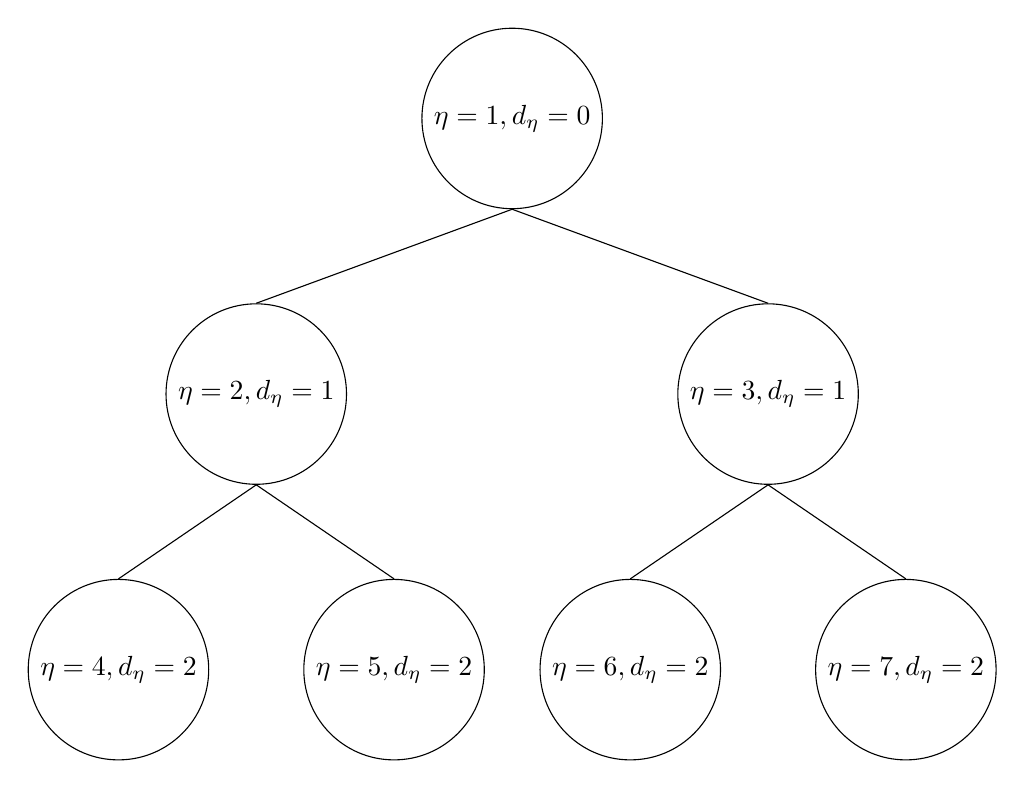
\begin{tikzpicture}
 \node [circle,draw]{$\eta=1,d_{\eta} =0$} [level distance=35mm,sibling distance=65mm]
child { node [circle,draw]{$\eta=2, d_{\eta} =1$} [level distance=35mm ,sibling distance=35mm]
child {node [circle,draw] {$\eta=4, d_{\eta} =2$}}
child {node [circle,draw]{$\eta=5, d_{\eta} =2$}}
}
child {node [circle,draw] {$\eta=3, d_{\eta} =1$} [level distance=35mm ,sibling distance=35mm]
child {node [circle,draw] {$\eta=6, d_{\eta} =2$}}
child {node [circle,draw]{$\eta=7, d_{\eta} =2$}}
};
\end{tikzpicture}

\caption{The binary heap node numbering system used in our simulations. }
\label{fig:tree_node_nums}  
\end{center}
\end{figure}
In addition to the process prior defined on the tree, we define a process prior on the selection of covariates for split rules within a tree. The function $\Pr{_{\text{rule}}}(\eta,j,r_j \vert \vec{q} )$ is decomposed into two components, one selecting the $j$th covariate which we use to propose a split at the node, and a second component selecting a specific split value ($r_j$). This corresponds to the conditional probability decomposition 

\begin{equation}\label{eqn:decomp}
\Pr{_\text{rule}}(\eta,j,r_j\vert \vec{q}) = \underbrace{\Pr{_\text{cov}}(j,\eta \vert \vec{q})}_{\text{ALN density}} \underbrace{\Pr{_\text{split value}}(r_j \vert j, \eta)}_{\text{Uniform}}.
\end{equation}

\noindent The tree prior, denoted $\Pr(\mathcal{T})$, is defined uniformly over the space of admissible trees. Exact enumeration of all admissible trees is only possible for very small values of $n$, the number of observations. The number of admissible trees is a cumulative sum of Catalan numbers less than or equal to a given depth. This sum grows at the rate $\mathcal{O}(4^n/n^{3/2})$ \cite{mattarei2009asymptotics}, the same rate as the Catalan numbers themselves, displayed in Figure \ref{fig:asymptotics}, and becomes intractable quickly. Fortunately, Markov chain Monte Carlo sampling allows us to sample from the space of trees using a Metropolis-Hastings rule with local proposals on the space of trees. We now detail the structure of the proposal functions. 

\begin{figure}[H]
  \centering
  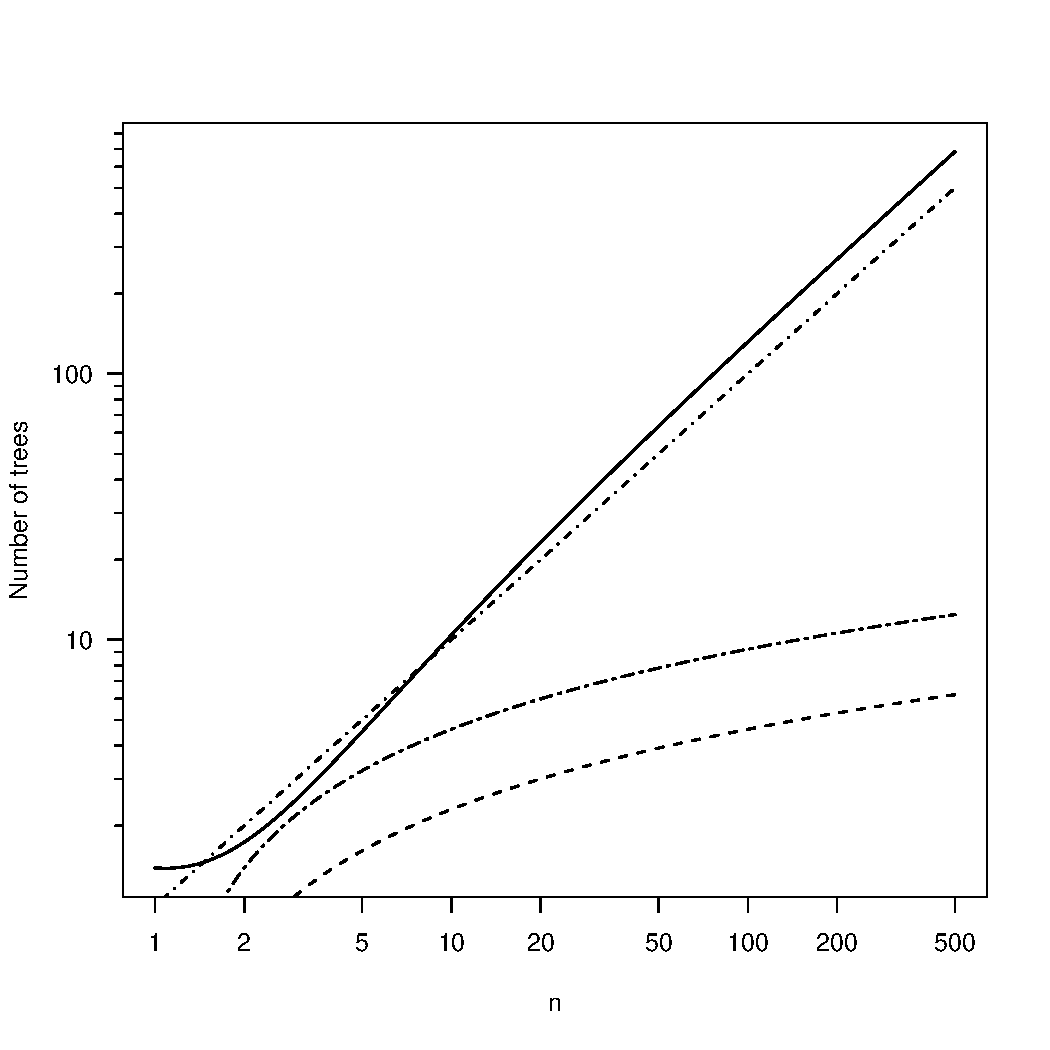
\includegraphics[width=4in]{figures/asymptotics_plot_bw.pdf}
  \caption{Plots of the log of the number of possible trees (solid line) less than or equal to a given depth $n$, compared to exponential (45 degree line), quadratic (dash-dotted line) and linear functions (even-dashed line). Note the vertical axis is on a log scale.  }
  \label{fig:asymptotics}
\end{figure}

Given a tree $\mathcal{T}$, we sample a new tree adjacent to $\mathcal{T}$ by proposing local updates. The local updates we use are the following: 

\begin{itemize}
 \item The Grow step: choose at random one of the terminal nodes and propose to append two new child nodes with probabilities given by Equation \ref{eqn:psplit}. 
 \item The Prune step: the reverse of the grow step, a terminal node is selected at random and the selected node and that selected node's sibling are both pruned to the immediate parent of the two child nodes. The parent node becomes a terminal node. 
 \item The Change step: randomly pick an internal node and propose to change the split rule at the selected node with that of another observation, possibly on a different covariate.
  \item The Swap step: randomly select an internal node that is not the immediate parent of any terminal node and proposes to swap the split rules of the parent-child pair. Otherwise, when both child nodes split on the same covariate, both child node's rules and the parent node's rules are swapped.
  \item The Rotate step: randomly choose a left or right rotation move, each with probability $1/2$. Then a rotatable node is chosen and a rotate move is performed.
 \end{itemize}
  The rotate operation for binary trees was first introduced in Sleator and Tarjan \cite{sleator1985self} and was implemented with Bayesian decision trees by Gramacy and Lee \cite{gramacy2008bayesian}. The rotate move was originally suggested by Knight, Kustra, and Tibshirani \cite{knight1998bayesian} as another possible move that might improve mixing. A good introduction and several practical uses of the rotate move can be found in Cormen, Lieserson, Rivest, and Stein \cite{cormen2001introduction}. The proposal functions in Gramacy and Lee \cite{gramacy2008bayesian} perform a rotate move only when a swap move is proposed and the parent-child pair both split on the same covariate. We modify this and allow rotate moves to be a separate proposal function and not a special swap move case. The proposal mechanism of Chipman et al. uses the grow, prune, change and swap moves only. In addition, neither Chipman et al. \cite{chipman1998bayesian}, Denison et al. \cite{denison1998bayesian}, nor Gramacy and Lee \cite{gramacy2008bayesian} included weights on each covariate in their examples or model specifications. They sampled each covariate and each split value uniformly across all covariates. 
  
\newpage


%% Chapter on DiVaS method 
 \section{Dirichlet Variable Selection For Decision Trees: The DiVaS method}
\label{ch:var_select}

%subsection{Introduction}
Many data analysis procedures, originally designed for inference in low dimensional spaces, create difficulties when dealing with high dimensional data.  Often data analysts use low dimensional intuition and apply similar logic to high dimensional data, which can often lead to erroneous conclusions. The approach outlined in this thesis not only moves around the high dimensional space efficiently, but also indicates with a high degree of probability which covariates are useful in determining the response at the tree nodes. In addition, we retrieve summary data indicating which dimensions are useful assisting the data analyst in the interpretation of results. Our primary focus in this thesis is on inferring a structural relationship between dimensions and the response of interest, with a preference towards interpretability. 

There are perhaps two predominant approaches to dealing with high dimensional data. The first attempts to only include dimensions that are important based on some metric of choice, usually with a filter run over the data to screen out some dimensions. Examples of this are principal components analysis \cite{tipping1999probabilistic} and various other approaches surveyed by Dash and Liu \cite{dash1997feature}. The second approach attempts to fit a model to the best dimensions sequentially. Examples of this approach include forward, backward and stagewise searches for regression models \cite{miller1984selection} \cite{myers1990classical} \cite{berk1978comparing}. The lasso \cite{tibshirani1996regression} is a problem which can be considered in either category, depending upon the approach taken. If we use the LARS algorithm to fit the model for all values of $\lambda$ then the method can be considered iterative. If instead, we fit a model for the lasso objective function choosing a single value of $\lambda$, for example by cross validation, then the method can be though of as a filtering approach. Our approach is similar to both approaches and operates by choosing a middle ground between these two extremes. As a byproduct of choosing this middle ground we are able to search the space of models more effectively and give intuitive summary results indicating which covariates are useful, while returning models to the analyst for use in prediction and inference. 

In this chapter we follow a \bayesorprob\ framework. We define a new prior measure over trees, which facilitates comparison across trees based on a global search of the tree space, and automatically induces coherent covariate selection. We assume a working familiarity with Markov chain Monte Carlo (MCMC) methods. For a good review of MCMC approaches to machine learning problems, we recommend the paper by Andrieu, De Freitas, Doucet and Jordan \cite{andrieu2003introduction}. We show through an example that greedily grown decision trees can fail to recover good trees in high dimensional data. Moreover, we find that previously implemented Bayesian approaches to decision tree learning have been applied only to low dimensional spaces \cite{chipman1998bayesian} \cite{gramacy2008bayesian} \cite{denison1998bayesian}. Applying the same approaches to high dimensional data is inappropriate and we demonstrate this through examples. These methods fail to move around the large dimensional space efficiently causing poor mixing and only finding local optima. 

Nearly all the previous approaches to decision tree induction have not explicitly incorporated model selection into the tree framework \cite{chipman1998bayesian} \cite{gramacy2008bayesian} \cite{denison1998bayesian} \cite{breiman1984classification} \cite{quinlan1993c4}. A notable exception is the recent paper by Gramacy and Taddy \cite{gramacy2012categorical} where binary indicators are used to perform model selection within a terminal node. Specifically, Gramacy and Taddy define a mixture of a Gaussian process (GP)\newabbrev{abbrev:GP} and the GP's limiting linear model, and use a point mass mixture to choose between the GP and the limiting linear model within each terminal node. This is in contrast with our approach, which aims to perform variable selection at the level of the decision tree itself and not for each model in each terminal node. Another notable exception is the work of Ishwaran, Kogalur, Gorodeski, Minn, and Lauer, who define a new quantity called a maximal subtree, and use the inherent topology of the tree and the maximal subtree to measure variable importance  \cite{ishwaran2010high}. Ishwaran et al. work in the context of random survival forests, built using bootstrapped data.  Most researchers have used implicit selection, for which predictors are chosen at the end of the greedy induction strategy as the predictors which are useful. Those not selected are considered not useful. Currently, most tree algorithms rely on a pruning rule for determining which covariates are useful. This implicit approach has the drawback of only providing ``yes/no'' answers to inclusion, and does not allow one to order the dimensions in some meaningful fashion. In our work we explicitly model these probabilities of inclusion and exclusion in the decision tree. This not only allows for useful predictor selection when choosing models, but also improves the efficiency of searching in large dimensions.  We note that we include a prune function in our proposal and this does affect the selection of which covariates are useful. However, in large dimensions, the more efficient way to improve the efficiency of the searching algorithm is to treat covariates differently based on their utility in the model. 

This chapter follows from the original Bayesian decision tree model of Chipman, George and Mcculloch \cite{chipman1998bayesian} (referred to hereafter as CGM), and Gramacy and Lee \cite{gramacy2008bayesian}(hereafter referred to as GL)\newabbrev{abbrev:GL}. Specifically, we propose a generalization of the models used by CGM and of GL. We allow rotate moves at all permissible nodes of the tree and varying selection probabilities on each covariate. In this manuscript we confine ourselves to categorical response data. All results can easily be extended and applied similarly to continuous data. In addition, we study the approach of CGM to large dimensional datasets. To our knowledge, the largest dimensions of data that the aforementioned approaches have been studied on are at most 15 dimensions. We find our method to be more effective than the CGM approach for large dimensional data. We also study the efficacy of a general rotate move in the transition kernel of the Markov chain.

The remainder of this paper unfolds as follows. Section \ref{sec:related_work} reviews previous greedy and Bayesian approaches to decision tree learning. Section \ref{sec:model_details} shows our model and describes how this is a modification of the algorithm proposed by CGM \cite{chipman1998bayesian}. In this and the next chapter we place emphasis on the algorithmic details of our procedure and only briefly describe some of the mathematical properties. Section \ref{sec:ecc} states necessary conditions for consistency of the decision trees we propose. Section \ref{sec:ase} shows how high dimensional data can create problems for both greedy and Bayesian approaches that have been previously proposed, and gives an example. Section \ref{sec:real_data} applies our approach to a dataset taken from the UCI machine learning repository. In Section \ref{sec:conc} we state conclusions and point towards future work.

\subsection{Related Work}\label{sec:related_work}
Some of the most well known approaches to decision tree learning are two approaches invented in the 1980's; these are Breiman, Friedman, Olshen, and Stone's cart method \cite{breiman1984classification} and Quinlan's C4.5 algorithms and variants \cite{quinlan1993c4}.  
The work of Breiman et al. \cite{breiman1984classification} showed the practical and theoretical approaches to decision tree induction. In Breiman et al. \cite{breiman1984classification}, the theoretical framework for discussing decision trees is given in terms of general impurity functions, allowing results to apply to specific impurities suggested by Quinlan \cite{quinlan1993c4}. For a theoretical treatment of consistency, the work of Devroye, Lugosi, and Gy\"{o}rfi \cite{devroye1996probabilistic} provided the foundation and application of the theory to certain tree methods.

The consistency of tree classifiers was also discussed by Breiman et al. \cite{breiman1984classification}. They showed that, under fairly general conditions, tree classifiers are asymptotically consistent, meaning trees can recapture the correct classifier if they are given enough data. The practical problem with this is that we usually only have a finite amount of data. Although we do not overcome this practical limitation, the results in Section \ref{sec:ecc} improve the rate of convergence by exploiting sparsity. Quinlan's approach modified the impurity functions proposed by Breiman \cite{breiman1984classification}, and also allowed for multiway splits at nodes in the tree \cite{quinlan1993c4}. Empirically, we have found that the entropy impurity function approach of Quinlan \cite{quinlan1993c4} performs better if there is a difference, although there is usually little or no difference in terms of the final tree. 

In our probabilistic approach, we quantify \emph{a priori} uncertainty in the classifier with a prior probability measure over trees. By defining a prior over trees, we induce a posterior distribution over trees via Bayes' rule shown in Equation \ref{bayesrule}, where $\theta$ denotes parameters in the model and $D$ denotes observed data.

\begin{equation}\label{bayesrule}
\Pr(\theta \vert D ) = \frac{\Pr(D\vert \theta )\Pr(\theta)}{\Pr(D)}
\end{equation}

 The posterior allows us to \emph{search} the space of trees, which is distinctly different from the greedy induction approach. In the Bayesian approach to decision tree induction several researchers have proposed various methods for searching over the tree space. The space of trees is a large discrete space, so MCMC algorithms are usually applied to search this space. CGM  \cite{chipman1998bayesian} proposed a clever process prior on the tree space, denoted $\Pr(\mathcal{T})$, to induce a posterior which moves between a varying number of dimensions. 
 %avoiding Reversible Jump moves
  Let $\mathcal{T}$ denote the tree and $\theta$ the collection of parameters in each terminal node (mean or class probabilities) and $D$ denotes data. Applying Bayes' rule, we have the result 
 \begin{equation}
 \label{eqn:tbup}
 \Pr(\mathcal{T}\vert D) = \frac{\int\Pr(D \vert \theta, \mathcal{T})\Pr(\theta\vert \mathcal{T})\Pr(\mathcal{T})d\theta}{\Pr(D)}.
 \end{equation}
 Note that the integral in the numerator of Equation \ref{eqn:tbup} treats the tree prior as a constant with respect to $\theta$. The integrated product of the other two quantities in the numerator is called the integrated likelihood and will be referred to in Section \ref{sec:model_details}. In the same year, Denison, Mallick, and Smith \cite{denison1998bayesian} proposed a reversible jump algorithm that has also shown success in searching tree space. As modifications to the work of CGM \cite{chipman1998bayesian}, GL \cite{gramacy2008bayesian} proposed a Gaussian process model in each terminal node, along with modifying the transition kernel to include rotations in one special case of swap moves. 
%\textbf{Need to figure out where this should go, not this section but somewhere in the first section (intro).}
%We focus on the work of CGM, and Gramacy and Lee \cite{gramacy2008bayesian}(hereafter referred to as GL). Specifically we propose a generalization of the transition kernel of GL allowing possible rotate moves at all permissible nodes of the tree. We do not however make an attempt to fit complicated functions in each terminal node. Instead we fit constant functions or choose the category with largest probability in the discrete outcome case. In addition, we study the approach of CGM to large dimensional datasets. To our knowledge the largest dimensions of data that the aforementioned approaches have been studied on is less than 15 dimensions. We study datasets with dimensions of size 100, 1000 and 1555. We study a real data set with 1555 dimensions and simulated datasets with 100 and 1000 dimensions. We find our method to be more effective than the CGM approach for large dimensional data. We also study the efficacy of the rotate move in the transition kernel of the Markov chain.

Bagging and boosting are two other common methods that might be used for performing model selection in the context of decision tree induction \cite{breiman1996bagging} \cite{freund1999short}. Often analysts will use these algorithms as black boxes and use the frequency of selected covariates in the resulting trees as measures of importance of decision trees. In the bagging context and the related random subspace method \cite{ho1998random}, one randomly subsamples either observations or dimensions and builds trees on this subsampled data. One of the difficulties with data containing many predictors is that, when we randomly sample with replacement collections of predictors to build trees, we select approximately 63\% of the dimensions \cite{efron1997improvements}. This is usually still a large feature space inheriting the same problems we initially faced. %Bagging and Boosting approaches have no theoretically justified measure to assess different models. Instead a holdout or cross validated estimate is often used to compare models based on prediction performance. Unlike in these two approaches, we have a measure to compare models. 
%Similar to these two approaches, we are able to search across many trees.
 Bagging and boosting methods are primarily used in the context of prediction. As initially stated, our primary motivation is on inferring a mechanistic relationship between dimensions and the response of interest with a preference towards simple and easily understood models. Hence, inference is the primary goal, with prediction being secondary. 

\subsection{Model Details}\label{sec:model_details}

In this section, after we define our approach, we detail the transition kernels proposed by CGM \cite{chipman1998bayesian} and by GL \cite{gramacy2008bayesian}. We highlight the differences between their approaches and our approach. 

Let us define the prior measure over a decision tree as
\begin{equation} 
\Pr(\mathcal{T}) = \prod_{\eta\in N} \Pr{_{\text{split}}} (\eta) \Pr{_{\text{rule}}}(\eta,s_k),\nonumber
\end{equation}
where $\eta$ ranges over all nodes in the tree, and the two probabilities are probabilities of a split at the node $\eta$, and the specific rule at node $\eta$, respectively. Also, $s_k$ denotes the randomly selected covariate. The probability of a split in a tree is 
 \begin{equation}
 \Pr{_\text{split}}(\eta)= \alpha(1+d_\eta)^{-\beta},\nonumber
 \end{equation}
where the quantities $\alpha>0$ and $\beta\geq0$ are parameters, and $d_\eta = \lfloor lg(\eta)\rfloor$ is the depth of the node $\eta$ under the usual binary heap node numbering (cf. Cormen, Lieserson, Rivest and Stein \cite{cormen2001introduction}). In this document $lg$ denotes a base 2 logarithm, and $log$ denotes a base $e$ logarithm. 
  
For our model we rely on the multinomial Dirichlet conjugate pair 
\begin{equation}
\small{\Pr(\underline{p})\Pr(c_i\vert \underline{p}) = \underbrace{K\prod_{i=1}^dp_i^{\alpha_i-1}}_\text{Dirichlet} \times \underbrace{{n \choose c_1,\dots ,c_d}\prod_{i=1}^dp_i^{c_i}}_\text{Multinomial}},\nonumber
\end{equation}    
where the $c_i$'s are  counts and $K$ is a normalizing constant. 

  The integrated likelihood quantity from the numerator of Equation \ref{eqn:tbup} is a multinomial Dirichlet conjugate pair. Therefore, the integral is available in closed form. We take the Dirichlet parameters ($\alpha_i$s) to be a vector of 1s although other alternatives are possible. The $\Pr_{\text{rule}}(\eta, s_k)$ is decomposed into two components, one selecting the $j$th covariate to use to propose a split at the node, and a second component selecting a specific split value. This corresponds to the conditional probability decomposition 

\begin{equation}\label{eqn:decomp}
\small{\Pr{_\text{rule}}(\eta,s_k) = \underbrace{\Pr{_\text{cov}}(s_k)}_{\text{multinomial}}\Pr{_\text{splitvalue}}(\eta \vert s_k)}.
\end{equation} 

The multinomial distribution in Equation \ref{eqn:decomp} to be a multinomial and we define a prior of choosing covariates to split on as a Dirichlet distribution. These two probability densities are conjugate pairs. This is brought about by assuming the structure $ \Pr{_\text{cov}}(s_k)\equiv\Pr{_\text{cov}}(s_k \vert s_{k-1}, s_{k-2},\dots, s_{1})$. To our knowledge, this refinement of the CGM model has not been employed in the literature. The work of Ishwaran et al. used the exact same breakdown as Equation \ref{eqn:decomp} but proposed a different probability density on the covariates. Also Ishwaran et al.'s method was used in the context of random survival trees, decision trees made using bootstrap sampled survival data \cite{ishwaran2010high}. 

When we sample a Markov chain we collect trees sampled under the dynamics of Equation \ref{eqn:MHrule}, a Metropolis-Hastings rule \cite{robert1999monte}. We often find that the observed counts of splits on each covariate drown out the information from the prior. This is an undesirable effect of the proposed model, because the observed split counts are not observed \emph{a priori}, but during the course of the MCMC algorithm. To combat this, we find it necessary to define the parameter $\widetilde{\alpha}$. This parameter is defined by setting the prior expectation of the probability of splitting proportional to the expectation of the unobserved split probabilities on a covariate written here in Equation \ref{eqn:constraint}

\begin{equation}\label{eqn:constraint}
\widetilde{\alpha} = \frac{C\sum_{j=1}^d\alpha_j}{\sum_{i,j}s_{ij}}.
\end{equation}
The $\alpha_j$ are the current concentration parameters of the Dirichlet distribution and $s_{ij}$ denotes the observed frequency of splits on dimension $j$ at iteration number $i$. This implies that the posterior for the covariate weights follows a modified Dirichlet distribution,
\begin{equation}\label{eqn:gen_dirichlet_dist}
\Pr(\underline{p}\vert \alpha, \underline{s}_i) = K(\widetilde{\alpha}){n\choose s_{i1}, \dots,s_{id}}\prod_{j=1}^dp_j^{\widetilde{\alpha}s_{ij}}.\nonumber
\end{equation}
Here $K(\widetilde{\alpha})$ is a normalizing constant. The extent to which the parameter $\widetilde{\alpha}$ (Equation \ref{eqn:constraint}) will impact the chain will depend on the length of each Markov chain. The parameter $\widetilde{\alpha}$ has a greater impact on chains that are run for a greater number of iterations.  

The constant $C$ in Equation \ref{eqn:constraint} must be greater than zero and is a specified constant governing the ratio of exploration and exploitation conducted on the covariates of the Markov chain. 
All MCMC algorithms have the property of exploring the space until a region of high posterior probability is found. Once found, the algorithm exploits the local concavity of this probability region. The extent to which an MCMC algorithm exploits and explores will determine how well the posterior distribution is recovered. The higher the value of $C$, the more exploration the Markov chain will conduct, and the smaller the value, the more exploitation.  In addition, for data sets of differing dimensions, we may wish to use the dimensionality to guide the choice of the exploration and exploitation. Larger dimensional data sets will require a larger value of $C$ to encourage exploration. If the analyst has good prior information in choosing $\alpha_j$'s, i.e. which covariates are useful, then the chain should move more towards exploitation, encouraging the Markov chain to find just the right splits and not focus too much on selecting the right covariates. 

The approaches of CGM and GL used discrete uniform probability masses on each covariate and on each available split value in the current node. We modify this by allowing the selection of covariates to vary from covariate to covariate, while keeping the discrete uniform prior on split values. We take the prior measure on the covariates to be a Dirichlet distribution and the observed counts for splits in the tree from the Markov chain as the pseudo counts of a multinomial likelihood.  Briefly, the benefits are:
\begin{itemize}
\item Improved searching of the Markov chain.
\item Better inferential and predictive trees. 
\item Easier interpretation of classifiers. 
\end{itemize}
We discuss the model and specification of parameters further in Section \ref{sec:ase} and in Chapter \ref{sec:real_data}.

The transition kernel describes the dynamics governing the state transitions of a Markov chain. To understand this let us introduce some notation, let $X^\prime$ denote the current state of the Markov chain, and $X$ some new future state. Then $k(X^\prime\vert X)$ denotes the probability of moving from the current state $X^\prime$ into the new state $X$, which may be viewed as a conditional density or mass function. In this paper, the states of the Markov chain are trees, denoted as$ \mathcal{T}^\prime $ (current) and $ \mathcal{T} $ (new). The transition kernel $k(\mathcal{T}^\prime\vert\mathcal{T})$ is defined by the Metropolis-Hastings rule 

 \begin{equation}\label{eqn:MHrule}
  \alpha(\mathcal{T}^\prime\vert\mathcal{T})= 
  min\left(1,\frac{ \Pr(\mathcal{T}\vert D)q(\mathcal{T}^\prime\vert\mathcal{T})}{ \Pr(\mathcal{T}^\prime\vert D)q(\mathcal{T}\vert\mathcal{T}^\prime)}\right). 
  \end{equation} 
  
 In Equation \ref{eqn:MHrule}, $q(\mathcal{T}^\prime\vert\mathcal{T})$ denotes a proposal function proposing a new tree $\mathcal{T}^\prime$, starting from the current tree $\mathcal{T}$. 
 Our proposal mechanism is as follows:
  \begin{itemize}
 \item The grow step chooses at random one of the terminal nodes and proposes to append two new child nodes with a certain probability that could depend on the tree depth, splitting on a chosen covariate.
 \item The prune step works in reverse of the grow, a terminal node is selected at random and that node and the node's sibling are pruned to the immediate parent of the two child nodes.
 \item The change step randomly picks an internal node and attempts to change the split rule at the node with that of another observation, possibly on a different covariate.
  \item The swap step randomly selects an internal node that is not the root node and proposes to swap the split rules of the parent-child pair. If both child nodes split on the same covariate, then both children and the parent node's rules are swapped.
  \item The rotate step randomly chooses a left or right rotation move. Then it randomly chooses an admissible internal node and rotates.
 \end{itemize}
 Sleater and Tarjan \cite{sleator1985self} introduced the rotate operation for binary trees in computer science. GL \cite{gramacy2008bayesian} first introduced the rotate operation into the Bayesian decision tree literature. A good introduction and several practical uses of the rotate move can be found in Cormen, Lieserson, Rivest and Stein \cite{cormen2001introduction}. The proposal of Gramacy and Lee \cite{gramacy2008bayesian} only allows a rotate move for the specific case when a swap move is proposed and the parent child pair both split on the same covariate. We modify this and allow rotate to be a separate operation of the transition kernel and not a special swap move case. The proposal mechanism of CGM uses the grow, prune, change and swap moves only. We also allow swap moves in our proposal. In addition, neither of these papers included weights on each covariate in their examples or model specifications. They sampled each covariate and split value uniformly at random. 

\subsection{Ensuring Consistent Classifiers}\label{sec:ecc}

In this section we aim to answer two questions. The first question is what is the behavior of our method as the number of dimensions $d \to \infty$. We generally tend to think of data as having a fixed dimensionality, but as data storage costs decrease, the number of variables tends to increase. We assume that the data has a large number of dimensions and use the theoretical quantity $d \to \infty$ as a guidepost. We use a working example throughout this section, a stump tree, which is a tree containing only one split rule. The second working example is a decision tree with an arbitrary number of splits. Through these two examples we see when the theory discussed in this section works and when the theory fails.  

We begin with a few definitions originally provided by Vapnik and Chervonekis \cite{vapnik1971uniform}, and subsequently studied by many others \cite{steele1978empirical} \cite{devroye1996probabilistic}. Let us define the shatter coefficient as the maximum number of sets obtained by intersecting a finite collection of points with functions from a specified class of functions and denote this as $s(\mathcal{A},n)$.\newnot{symbol:shatter_coef} For our work it will suffice to look at half spaces on $\mathbb{R}^d$, which have shatter coefficient $2^n$ for $n<d$, but once $n>d$, the shatter coefficient no longer grows exponentially, instead growing polynomially in n. We say a class of functions $\mathcal{A}$ has Vapnik-Chervonekis (VC)\newabbrev{abbrev:VC} dimension $V_\mathcal{A}$,\newnot{symbol:VC_dim} where $V_\mathcal{A}$ denotes the largest value in the \emph{exponent} of the shatter coefficient, such that the exponent equals the sample size. Formally, let us define this value as $V_\mathcal{A}\overset{def}{=}max\{n:s(\mathcal{A},n)=2^n\}$. Intuitively, the VC dimension denotes a phase change in the shattering dynamics as a function of the sample size, as seen, for example, in Figure \ref{fig:phase_change_shatter_dynamics}. This phase change occurs when the growth in the shatter coefficient as a function of $n$, the sample size, changes from exponential to polynomial. For half spaces on $\mathbb{R}^d$, $V_\mathcal{A}=d$ \cite{devroye1996probabilistic}. We will use the shatter coefficient and VC dimension in error bounds stated in this section.  


\begin{figure}[h]
\centering
  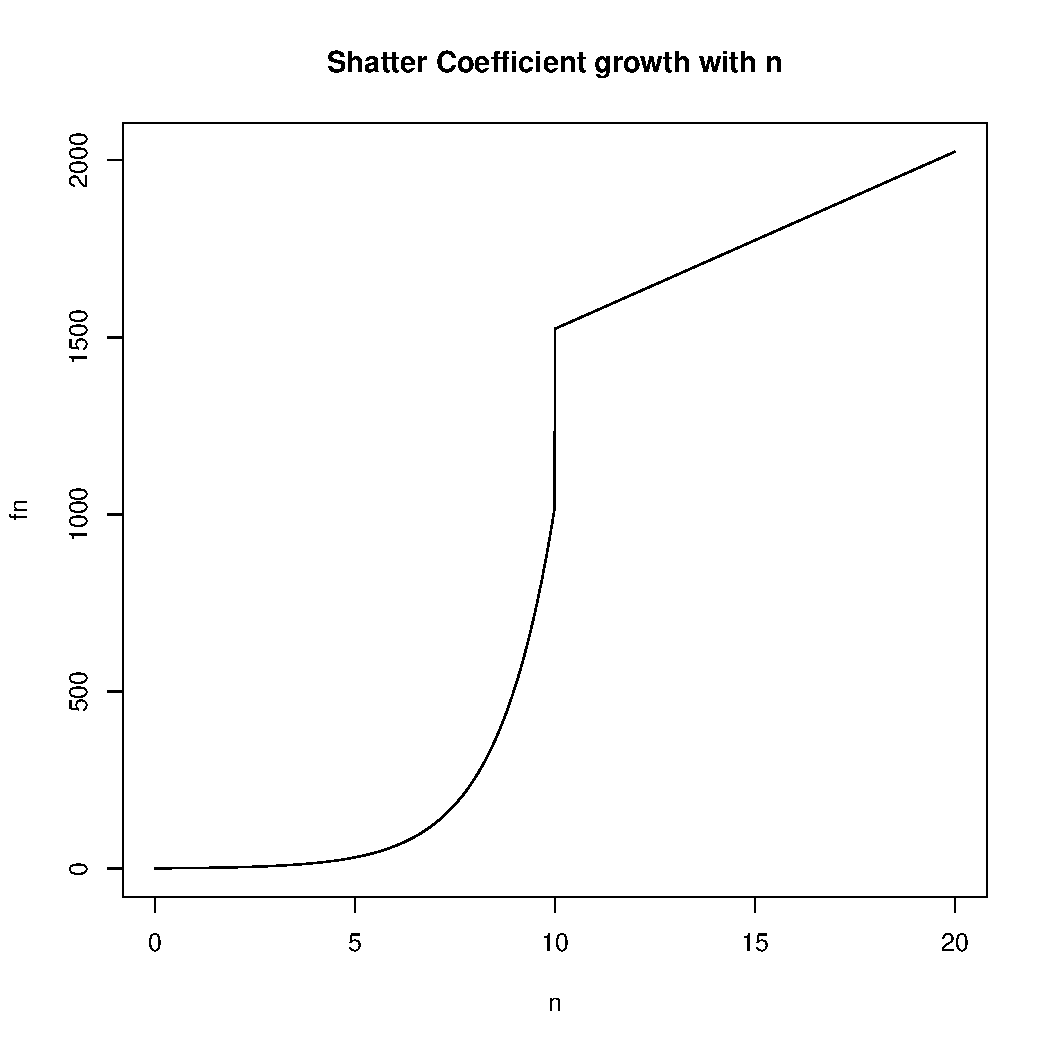
\includegraphics[scale=0.7]{figures/phase_change_shatter_dynamics.pdf}
  \caption[A shatter coefficient plot]{The shatter coefficient function for half spaces in $\mathbb{R}^d$, as a function of $n$. In this plot $d=10$.}\label{fig:phase_change_shatter_dynamics}
\end{figure}

Devroye, Gy\"{o}rfi, and Lugosi \cite{devroye1996probabilistic} provided the following result: 

\noindent \textbf{Theorem 1}\\
For $0<k^2 /(k-1)< n\varepsilon^2$,
\begin{equation}\label{eqn:vcb}
\Pr\left(\underset{A\in \mathcal{A}}{sup} \vert v_n -v\vert > \varepsilon\right) \leq 4ks(\mathcal{A},n)\exp\vspace{-.1in}\left[\frac{-n\varepsilon^2}{2k^2}\right].
\end{equation}

The notation $v_n \overset{def}{=}(1/n)\sum_{i=1}^n\mathds{1}(y_i =\hat{\mathcal{T}}(X_i))$ \newnot{symbol:empirical_error}denotes the empirical error of the estimated classifier and the notation $v\overset{def}{=}\Pr(\mathcal{T}(X)=y)$\newnot{symbol:true_error} denotes the Bayes error of the data. This result tells us that if the family of classifiers has a finite VC dimension, or equivalently a finite shatter coefficient, then the classifier is consistent. Here $k$ and $\varepsilon$ are specified constants, usually we take $k=2$ and $\varepsilon=0.01$. Now we know that a halfspace split in $\mathbb{R}^d$ has $V_\mathcal{A}=d$. Let us define \newnot{symbol:entropy}$\mathcal{H}(x) = -xlog(x) -(1-x)log(1-x))$ for $0 \leq x \leq 1$ with $\mathcal{H}(1)=\mathcal{H}(0)=0$. A useful inequality is 

\begin{equation} 
s(\mathcal{A},n)\leq \exp[n\mathcal{H}(V_\mathcal{A}/n)],
\end{equation}
 for $V_\mathcal{A} < 2n$. We see that, for $d<2n$, this inequality holds and, thus, the right hand side of inequality \ref{eqn:vcb} will go to $0$, as $n\to\infty$. For our stump, the tree will capture the Bayes error as $n\to\infty$, if the model is correct. We also see that, for $n<d$, the shatter coefficient for half spaces is $2^n$. If $d\to\infty$ and $n\to\infty$, but $n<d$, we have no consistency guarantee, according to this bound.  In the second case, let us consider a decision tree of arbitrary depth. Theorem 13.5 of Devroye, Gy\"{o}rfi, and Lugosi tells us that for $\mathcal{A} =\{ \mathcal{A}_1 \cap \mathcal{A}_2\}$, 

 \begin{equation}
  s(\mathcal{A},n) \leq s(\mathcal{A}_1,n)s(\mathcal{A}_2,n).
\end{equation}

For decision trees with two splits on halfspaces, the shatter coefficient is bounded above by $2^{2n}=4^n$, for sample sizes less than $d$. For sample sizes larger than $d$ we will have consistency as $n\to\infty$, provided that the decision tree does not grow arbitrarily large. As a simple requirement we ensure that the trees do not grow arbitrarily large, by ensuring that trees are shallower than $K$, for some constant $K$. Note that this constraint was also required by Denison, Mallick and Smith's reversible jump algorithm \cite{denison1998bayesian}. Our simulation studies indicate that there is little to no sensitivity in the specification of $K$. Figures \ref{fig:depth2} -\ref{fig:depth10} show the results of simulating from the posterior distribution over trees and varying the maximum depth, $K$. We evaluate for values of $K=2,3,4,5,6,7,10$. For small values of $K$ such as 2 or 3, the setting of maximum depth appears to limit the sampler from exploring possible trees.  However, once $K$ is set larger than 6 there appears to be little impact restricting the sampler from exploring certain trees. Of course, for any given data set the value of $K$ that is acceptable will likely change, so our conclusion is that $K$ should be large enough. Our assumption is $K=20$ or $K=30$ should be enough for most problems. Simply stated, $K$ should be large. Too small values of $K$ can cause problems. A value of $K=10$ appears sufficient for our purposes and causes no problems. 

  \begin{figure}[h]
  \minipage{0.35\textwidth}%
  \centering
  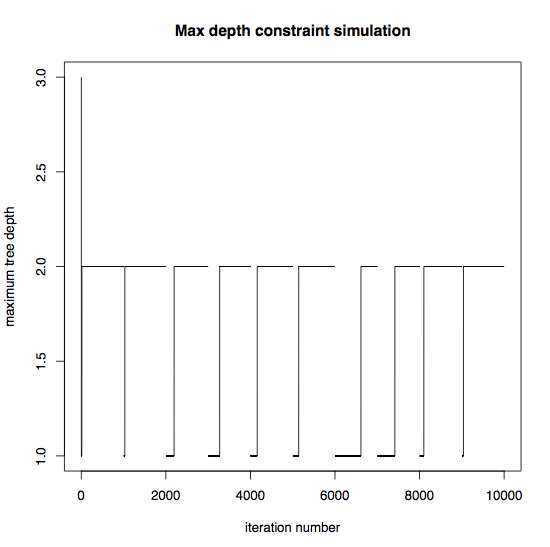
\includegraphics[scale=0.4]{mdepth2.png}
  \caption[Maximum depth of samplers trees with maximum depth set at 2]{Maximum depth of samplers trees with maximum depth set at 2.}\label{fig:depth2}
\endminipage\hfill
\minipage{0.35\textwidth}%
  \centering
 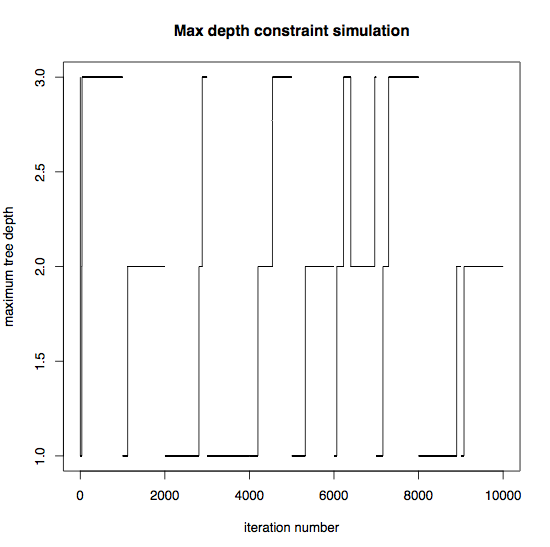
\includegraphics[scale=0.4]{mdepth3.png}
  \caption[Maximum depth of samplers trees with maximum depth set at 3]{Maximum depth of samplers trees with maximum depth set at 3.}\label{fig:depth3}
\endminipage
\end{figure}

  \begin{figure}[h]
  \minipage{0.35\textwidth}%
  \centering
  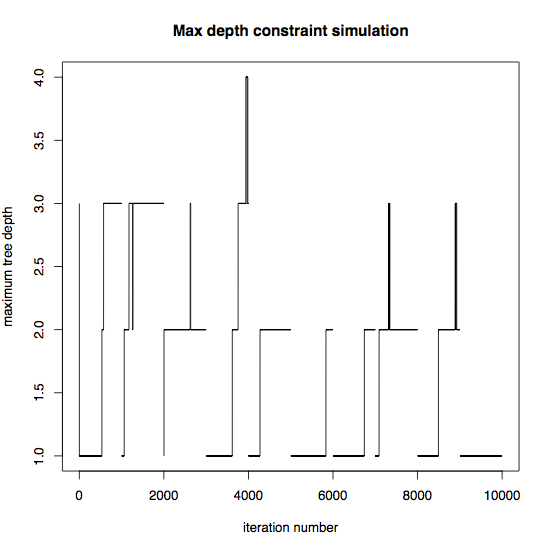
\includegraphics[scale=0.4]{mdepth4.png}
  \caption[Maximum depth of samplers trees with maximum depth set at 4]{Maximum depth of samplers trees with maximum depth set at 4.}\label{fig:depth4}
\endminipage\hfill
\minipage{0.35\textwidth}%
  \centering
 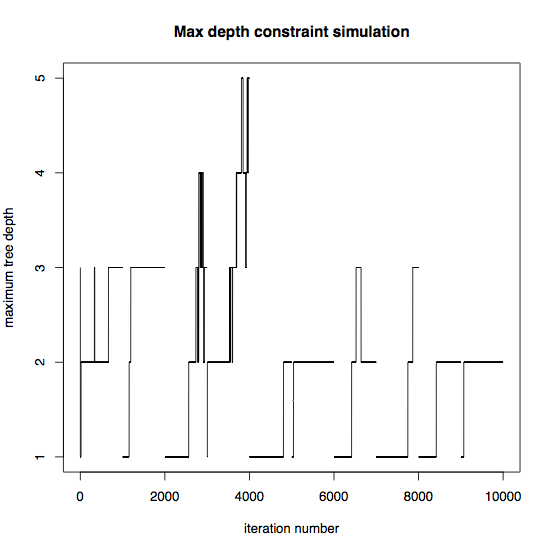
\includegraphics[scale=0.4]{mdepth5.png}
  \caption[Maximum depth of samplers trees with maximum depth set at 5]{Maximum depth of samplers trees with maximum depth set at 5.}\label{fig:depth4}
\endminipage
\end{figure}

  \begin{figure}[h]
  \minipage{0.35\textwidth}%
  \centering
  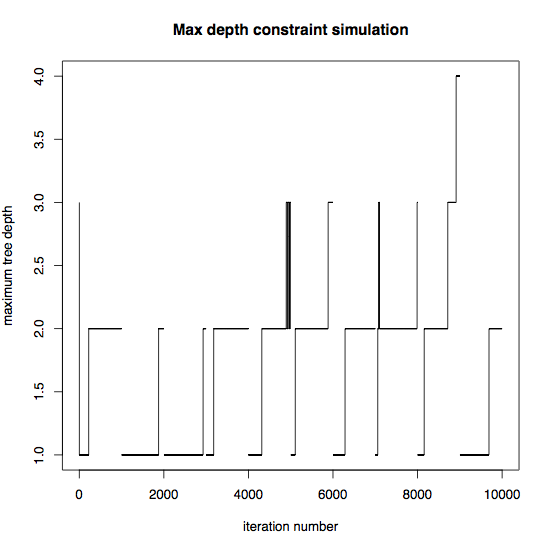
\includegraphics[scale=0.4]{mdepth6.png}
  \caption[Maximum depth of samplers trees with maximum depth set at 6]{Maximum depth of samplers trees with maximum depth set at 6.}\label{fig:depth6}
\endminipage\hfill
\minipage{0.35\textwidth}%
  \centering
 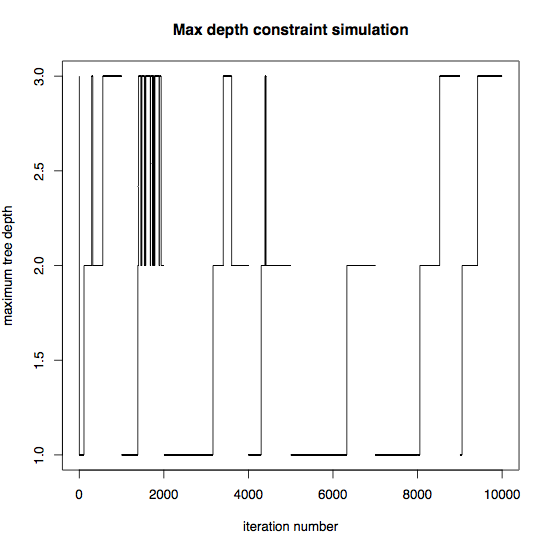
\includegraphics[scale=0.4]{mdepth7.png}
  \caption[Maximum depth of samplers trees with maximum depth set at 7]{Maximum depth of samplers trees with maximum depth set at 7.}\label{fig:depth7}
\endminipage
\end{figure}

  \begin{figure}[h]
  \centering
  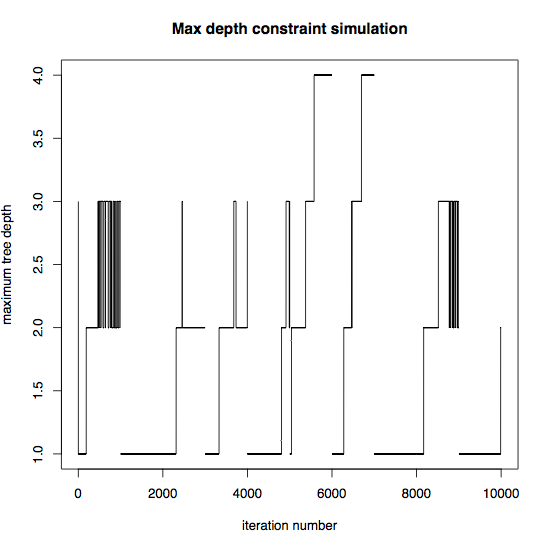
\includegraphics[scale=0.4]{mdepth10.png}
  \caption[Maximum depth of samplers trees with maximum depth set at 10]{Maximum depth of samplers trees with maximum depth set at 10.}\label{fig:depth10}
\end{figure}


Up to this point, the material in this section is nothing new, but contained fully in the work of Devroye, Gy\"{o}rfi, and Lugosi. Now let us define the sparse shatter coefficient as the shatter coefficient using only dimensions where $S_j =1$, denoted $s(\mathcal{A},n\vert S_{j=1}^d))$ and $S_j \in \{0,1\}$. We now use this sparse definition to carry over results into cases where sparsity holds in classification problems. \\
 
 \textbf{Theorem 2}\\
For $0<k^2 /(k-1)< n\varepsilon^2$ and $\mathbb{E}(S_j)=p_j$, the bound 

\begin{equation}\label{eqn:sparse_vcb}
\small{\Pr\hspace{-.04in}\left(\underset{A\in \mathcal{A}}{sup} \vert v_n -v\vert > \varepsilon\right)\hspace{-.05in} \leq 4ks(\mathcal{A},n\vert S_{j=1}^d))\exp\hspace{-.05in}\left[\frac{-n\varepsilon^2}{2k^2}\right]}
\end{equation} 
holds, if and only if $\sum_{j=1}^dp_j < \infty$, where $d$ can be finite or infinite.
 In the case $d<\infty$ everything looks nearly the same and the proof follows verbatim from the derivation in Devroye, Gy\"{o}rfi, and Lugosi. The case $d=\infty$ is delicate and requires Kolmogorov's three series theorem \cite{loeve1977probability}.    

The second error bound (Equation \ref{eqn:sparse_vcb}) differs from the first (Equation \ref{eqn:vcb}) in that now we are only using some subset of the covariates to classify the observations. Explicitly, the number of effective dimensions, denoted as $d^*$, can be bounded almost surely, but the total number of dimensions $d\to\infty$. Each $S_j \in \{0,1\}$, so if $\Pr(S_j=1)=1$, then we are back into the case of the first theorem, which is non sparse shattering. In our case, we relax the assumption that all $\Pr(S_j=1)=1$ and instead allow $\Pr(S_j=1)=p_j$, for $0\leq p_j\leq 1$. This can be thought of as a convex relaxation of a non-convex, computationally difficult optimization problem. The sum $\sum_j^dS_j$ is now a random sum, since each $S_j$ is a random variable. Also, this random sum is the sparse VC dimension for splits of the form $(\infty, a_i]$, the splits we use to construct our classifiers. Passing to the limit as $d\to \infty$, we want the random infinite series to converge, otherwise we will not have a consistent classifier. The Kolmogorov three series theorem tells us that convergence almost surely of the random series $\sum_{j=1}^\infty S_j$ occurs if and only if the series $\sum_{j=1}^\infty p_j$ converges, thus necessary and sufficient conditions are $\sum_{j=1}^\infty p_j < \infty$. 

We have necessary and sufficient conditions for convergence and therefore for consistency of our sparse classifier in infinite dimensional data. We need only ensure that $\sum_{j=1}^\infty p_j < \infty$. Provided $\sum_{j=1}^\infty p_j <\infty$ the stump tree will be consistent with infinite dimensional data as $n\to\infty$ Furthermore, the tree with arbitrary but finite depth will also be consistent, provided that the tree does not grow too deep, less than $2^K$ for some large but finite $K$. Intuitively this result should make sense. For infinite dimensional data, we must have most dimensions be irrelevant for the classification task, in order for the resulting classifiers to be consistent. In other words, most $p_j \to 0$ and some $p_{j^\prime}\to c >0$ ($0<c<1$) as $d\to\infty$. Our approach, without the $\widetilde{\alpha}$, ensures precisely this condition. Furthermore, this is not a weakness of our approach, because this theoretical result holds for $d\to\infty$. In our real data cases $d$ is finite and usually fixed. The $\widetilde{\alpha}$ is a practical aspect of our approach and is used to improve exploration and exploitation in fixed, finite dimensional data. 

\subsection{A Simulated Example}\label{sec:ase}

This section details a simulated example where we know which covariates are important and which are not important. Of course, this will never be the case in practice, yet, for verification, we find this setting useful. 

For our example, we note that a greedily built decision tree with a linear classifier can universally fail, if we are willing to make $d$ large enough. To accomplish this for each covariate after $d^*$, we will simulate from a mixture of two normals, where each mixing probability is $1/2$, and the means of the two normals are taken from a continuous uniform distribution on a large enough region $(l,u)$. If we can generate data where each covariate has observations in two groups that are separated enough and some of the responses are also separated, then we will incorrectly select a split rule based on this covariate, when in reality this covariate is independent of the response by construction. This will occur more frequently for larger $d$. Fortunately, our method will still select the correct covariates and as a result, select the correct tree.   

 Let us define the data generating process (DGP)\newabbrev{abbrev:DGP} as that given in Figure \ref{fig:awesome_image2}.  

\begin{figure}[h]
\centering
\label{fig:3fig_tree}
  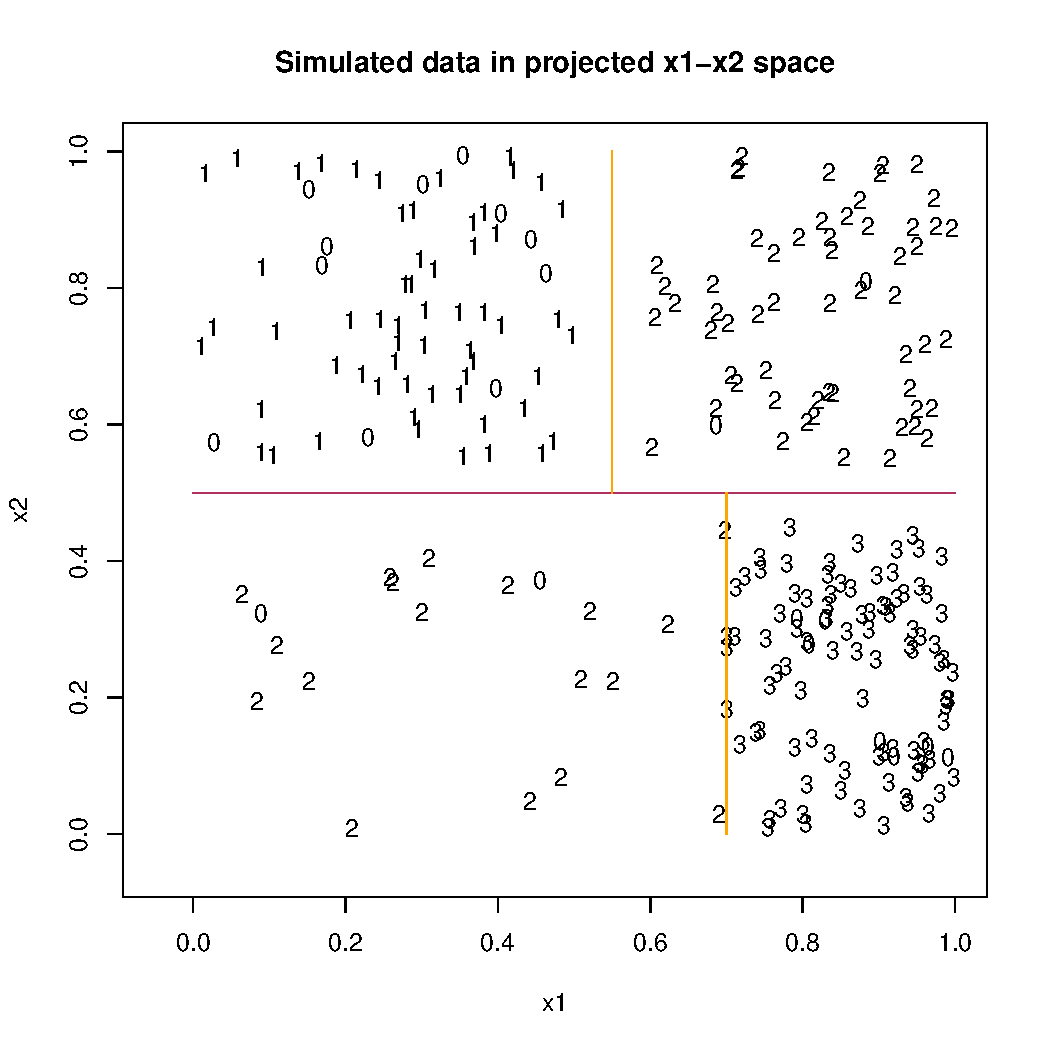
\includegraphics[scale=0.4]{figures/proj_plot.pdf}
  \caption{A plot of the true DGP}\label{fig:awesome_image2}
\end{figure}

The probability of being the majority class in any of the four regions of the Figure \ref{fig:awesome_image2} is 90\%. Therefore no perfect classifier exists, yet very good classifiers are possible.
We next generate additional covariates independently according to the mixture strategy described in the previous paragraph, with the continuous uniform supported on the interval $(0,20)$. We look at the cases of $d=100 \text{ and } 400$. The trees generated by the three tree methods are shown in Figures \ref{fig:awesome_image1}-\ref{fig:awesome_image3}. The best tree found by our method is the generative tree of the data, and therefore this classifier achieves the Bayes' error rate for this example. We simulate several Markov chains are simulated to guard against trapping in local optima. This is not a new strategy for MCMC with many local optima and was proposed by CGM \cite{chipman1998bayesian} for decision tree MCMC samplers to aid exploration of the decision tree space and to prevent getting stuck in one of the many local optima.  We tried a few chain lengths (500, 1000, and 2000) of each chain and reran 10 chains on each data set. The results were the same, regardless of the chain length.

\begin{figure}[h]
\centering
\label{fig:3fig_tree}
  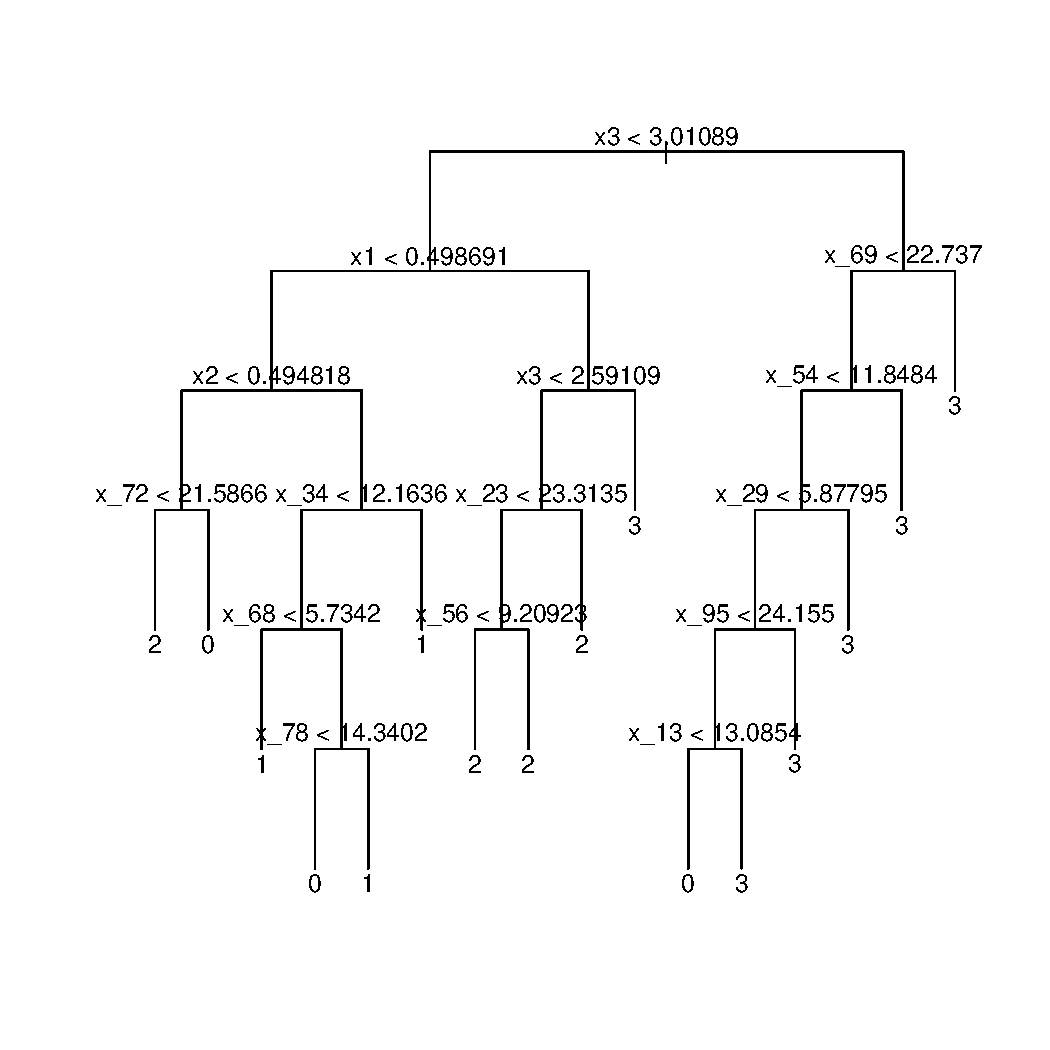
\includegraphics[scale=0.4]{threetree1.pdf}
  \caption{The tree found by a greedy optimization}\label{fig:awesome_image1}
  \end{figure}
  \begin{figure}[h]
  \minipage{0.35\textwidth}%
  \centering
  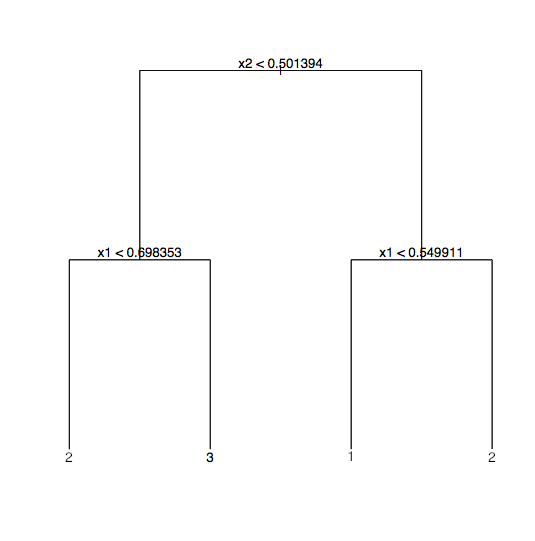
\includegraphics[scale=0.4]{figures/simul_example_map_tree_USE.png}
  \caption{Best tree using the weighted method}\label{fig:awesome_image4}
\endminipage\hfill
\minipage{0.35\textwidth}%
  \centering
 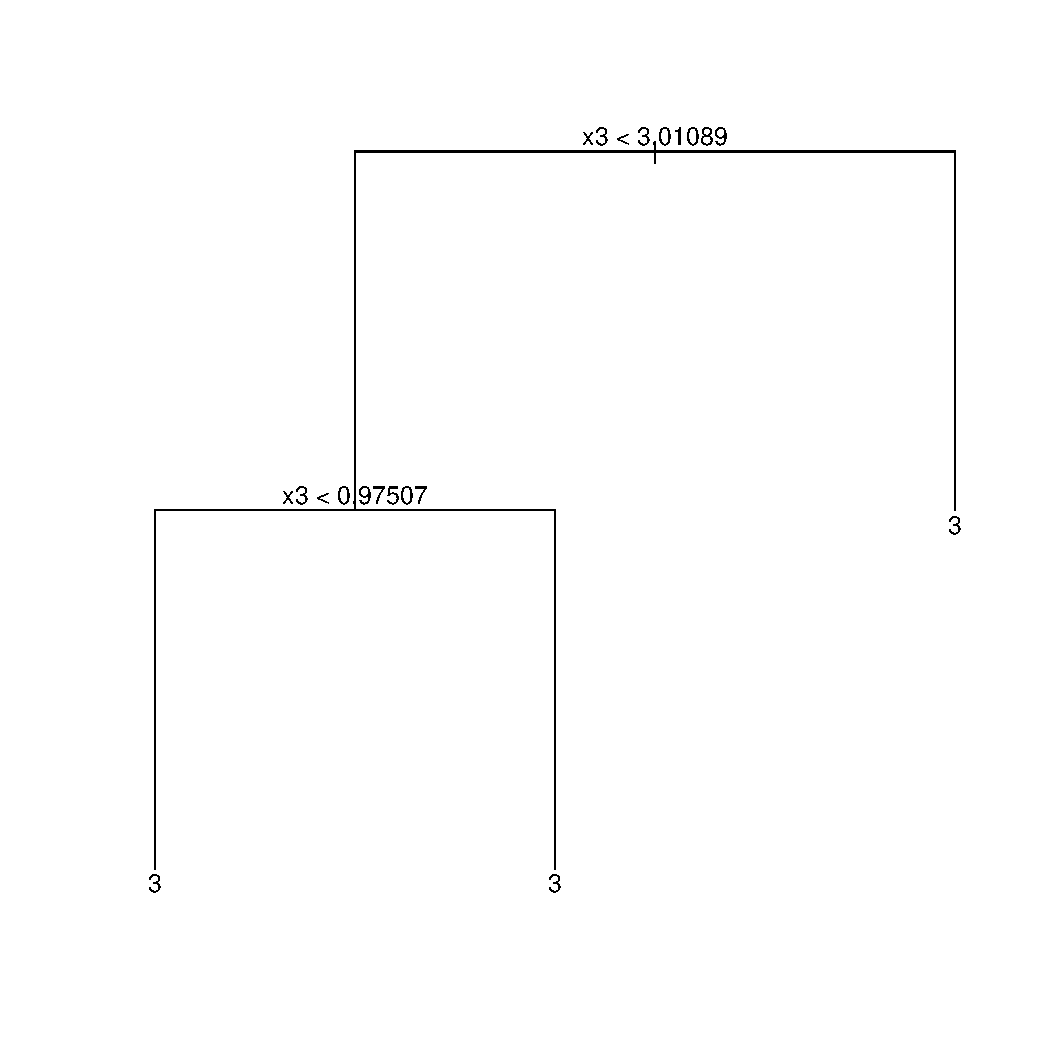
\includegraphics[scale=0.4]{figures/cgm_tree_simul.pdf}
  \caption{The best tree found by the CGM method}\label{fig:awesome_image3}
\endminipage
\end{figure}
\begin{figure}[h]
\centering
\label{fig:3fig_tree}
\minipage{0.35\textwidth}
\centering
  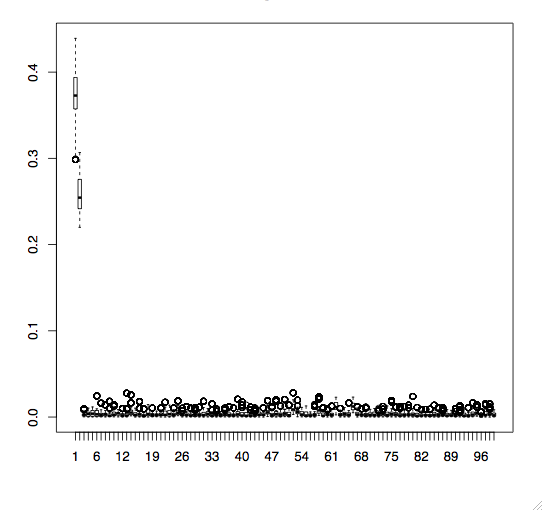
\includegraphics[scale=0.4]{figures/weight_simulated_example_USE1.png}
  \caption[Covariate inclusion probabilities for the 100 covariate example]{Covariate weights on the 100 dimensional example. Note the first two covariates are selected with high probability and the rest with miniscule probability.}\label{fig:awesome_image5}
\endminipage\hfill
\minipage{0.35\textwidth}
\centering
  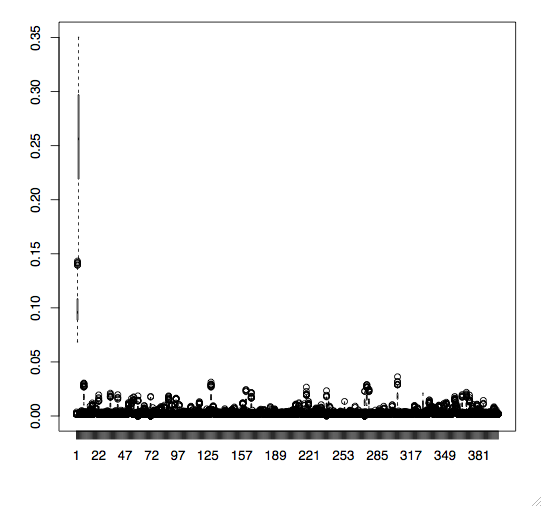
\includegraphics[scale=0.4]{figures/my_method1.png}
  \caption[Covariate inclusion probabilities for the 400 covariate example]{Covariate weights on the 400 dimension simulated example. Note the first two covariates are selected with high probability and the rest with negligible probability.}\label{fig:awesome_image6}
\endminipage\hfill
\end{figure}
\begin{table}[h]\footnotesize
\centering
  \begin{tabular}{| c | c | c }
  \hline 
Method & Misclass Prob.\\
      \hline 
Greedy &   11.6\%    \\
 CGM &     62.4\% \\
   Weighted & 10.8\%   \\
      \hline
  \end{tabular}
    \caption[Misclassification probabilities for $d=100$]{Misclassification probabilities of the three tree fitting methods for $d=100$.}
  \label{tab:sim_misclass1}
\centering
\end{table}

\begin{table}[h]\footnotesize
\centering
  \begin{tabular}{| c | c | c }
  \hline 
Method & Misclass Prob.\\
      \hline 
Greedy &  24.8\%     \\
 CGM &    57.2\% \\
   Weighted &  10.0\%  \\
      \hline
  \end{tabular}
    \caption[Misclassification Probabilities of the three tree fitting methods for $d=400$]{Misclassification Probabilities of the three tree fitting methods for $d=400$.}
  \label{tab:sim_misclass2}
\centering
\end{table}


To compare the three methods, we calculate misclassification probabilities for each of the three methods. To calculate misclassification probabilities we took a random sample of 250 observations as hold out test data. The misclassification probabilities are calculated by dropping all data points from the test data set through the resulting trees. We fit the trees using only the 250 observations from the training data. The tables of misclassification probabilities are displayed in Tables \ref{tab:sim_misclass1} and \ref{tab:sim_misclass2}.

We see that the pruning rule fails to collect the correct covariates as important in the greedily grown tree. The problem is that the deterministic procedure is overwhelmed by candidate splits and thus overfits, in fact the misclassification probability \emph{within} the training data is 4.8\%, better than the Bayes rate! However, this method performed poorly on hold out data compared to the weighted method, as shown in Tables \ref{tab:sim_misclass1} and \ref{tab:sim_misclass2}. The greedy method eventually finds some suboptimal splits. Of course, in this example we know the truth, and these extra splits are far from the truth. In addition, we see that the CGM approach fails on these trees. Much like the greedy method, the CGM approach is also overwhelmed with possible splits. Each new covariate adds exponentially more possible trees. This plethora of trees often allows one to find many locally optimal trees, but at the cost of exponentially more search time. A benefit of our method is the improved search by effectively ignoring certain covariates and preventing some trapping of the chain in local optima. By allowing non-uniform probabilities of selecting covariates, the algorithm spends more time searching through covariates that have good splits, while not spending time in other covariates that have mostly useless splits. This behavior leads to a more efficient search of the tree space and, consequently, better predictive trees than those found by the CGM search approach.A s indicated by the results in Table \ref{tab:sim_misclass2}, the trees built using our weighted approach are better or competitive in prediction but simpler for inference compared with those found by a greedy search. 

\subsubsection{Choosing Covariates}
A natural question to ask is: How should one choose covariates? This question is important because there are often covariates which have estimated probabilities which might be considered large enough to be important but also could be small enough to be considered   not important. We approach this question from the context of the learning achieved during the sampling. We call the prior moment estimator defined here by Equation \ref{eqn:mom_est_dirichlet} as

\begin{equation}\label{eqn:mom_est_dirichlet}
\Pr(\text{covariate $j$ included})= \frac{\alpha_j}{\sum_{j=1}^d \alpha_j}.
\end{equation}

Nonetheless, the prior moment estimator does not take into account the learning performed by the MCMC algorithm. We now discuss a method that accounts for the learning occurring as the MCMC algorithm progresses.

Note that Equation \ref{eqn:mom_est_dirichlet} is simply the maximum likelihood estimator of the \emph{a priori} probabilities of each covariate being selected to split on in the decision tree. To choose which covariates to use (in some subsequent model building), one might select those covariates where the \emph{a posteriori} probabilities are larger than the \emph{a priori} probabilities. This then indicates that information on the covariates was learned during the course of the MCMC algorithm. Formally, select the set of covariates for inclusion according to the rule 

\begin{equation}\label{eqn:cov_inclusion_rule}
 J = \left\{ \text{all } j:\frac{\alpha^\prime_j}{\sum_{j=1}^d\alpha^\prime_j}>  \frac{\alpha_j}{\sum_{j=1}^d\alpha_j } \right\},
\end{equation}

 where the $\alpha_j^\prime = \alpha_j +\widetilde{\alpha}s_j$ denote posterior concentration parameters for each covariate.
 
 Other methods for covariate selection are possible but we do not discuss them here. 
We present a small simulation study to determine the efficacy of the proposed method. We simulate data as described in the earlier portion of this section, where we know the specified covariates that should be selected, and those that should not. We ran the simulation 100 times and present the average percentage correctly selected by using the rule in Equation \ref{eqn:cov_inclusion_rule} for our weighted method. We also compared our weighted method results to simple frequency estimates using bootstrap samples and using the CGM method for fitting decision trees. The results are presented in Table \ref{tab:sim_study}. We fit a collection of trees using a bootstrap resample of 100 and using 1000 trees and calculate the number of times the correct covariates are selected. These entries are the subscripted `100' and `1000' entries in Table \ref{tab:sim_study}. 

% \begin{table}[h]\centering
%  \begin{tabular}{| c | c  c  c  c  c |}  \hline 
%
%      \hline 
%$\Pr(\text{covariate 1 selected})$ & - & - & - & - & - \\
%$\Pr(\text{covariate 2 selected})$&  - & - & - & - & - \\
% $\Pr(\text{ covariates 1 and 2 selected})$&  - & - & - & - & - \\
%$\Pr(\text{any other covariates  selected})$&  - & - & - & - & - \\
%   \hline
%  \end{tabular}
%  \caption{The empirical performance of the tree fitting methods on the variable selection problem using 100 simulations.}
%  \label{tab:sim_study}
%\centering
%\end{table}

% latex table generated in R 2.15.0 by xtable 1.7-0 package
% Thu Feb 21 09:12:06 2013

\begin{table}[ht]
\begin{center}
\begin{tabular}{l | rrrrr}
  \hline
  & Weights & Boot$_{100}$ & Boot$_{1000}$ & Greedy & CGM \\ 
  \hline
$\Pr(\text{covariate 1 selected})$ & 0.32140 & 0.12405 & 0.12664 & 0.12178 & 0.13333 \\ 
$\Pr(\text{covariate 2 selected})$ & 0.33806 & 0.10795 & 0.10835 & 0.12376 & 0.06667 \\ 
  $\Pr(\text{covariates 1 and 2 selected})$& 0.15429 & 0.08712 & 0.08365 & 0.08614 & 0.06667 \\ 
  $\Pr(\text{any other covariates  selected})$ & 0.34054 & 0.76799 & 0.76502 & 0.75446 & 0.80000 \\ 
   \hline
\end{tabular}
 \caption[Empirical covariate selection with 100 simulations]{The empirical performance of the tree fitting methods on the variable selection problem using 100 simulations.}
 \label{tab:sim_study}
 \end{center}
\end{table}


From Table \ref{tab:sim_study} it is clear that the weighted method outperforms the four other methods in correctly selecting the important covariates. Also, our weighted method selects the correct covariates jointly better than the other methods. Moreover, our weighted method selects incorrect covariates less often. whereas the other methods have a higher frequency of incorrectly selecting covariates. It is important to note that theoretically we do not want the entries in the last line to approach zero. If we did this then the MCMC would get immediately stuck in a local maximum of the likelihood space and would not find many good local maxima. Our weighted method is able to more evenly balance the search for new local maxima with the search for the correct splits and tree topology within the basin of attraction of the current local maximum. This leads to improved searching of the tree space and leads to better trees in terms of inference, which are competitive in terms of prediction.  

\section{A Case Study of the DiVaS Model}\label{sec:real_data}
In this section we compare our method against the greedy approach and the CGM approach using the publicly available internet ads dataset from the UCI data repository \cite{Frank:2010uq}. The internet ads data set contains 1558 covariates, some numeric and some categorical. The data set was first used in a paper by Kushmerick \cite{kushmerick1999learning} and has since been used in several statistical classification studies. The UCI machine learning repository contains a more complete listing of papers using this dataset. 

As noted by Kushmerick \cite{kushmerick1999learning}, there are several reasons for wanting to remove advertisements from webpages. Some reasons are: Images tend to dominate a page�s total download time, users dislike paying for services indirectly through advertisers, preferring direct payment for services rendered, and malicious software can be unintentionally placed on a user's machine through images masked as advertisements. 

We used a random subset of internet advertisements data to fit a greedy tree, a CGM tree and a tree fit using our weighted method. We first removed all observations that contain missing values. We then took a 50\% random sample of training and test data. The resulting trees are shown in Figures \ref{fig:ads_image1}-\ref{fig:ads_image3}. The misclassification probabilities are calculated by dropping all data points from the test data set through the trees built using the training data. The resulting trees are fit using only the training data.  
\begin{figure}[h]
\label{fig:3fig_tree}
\minipage{0.35\textwidth}
  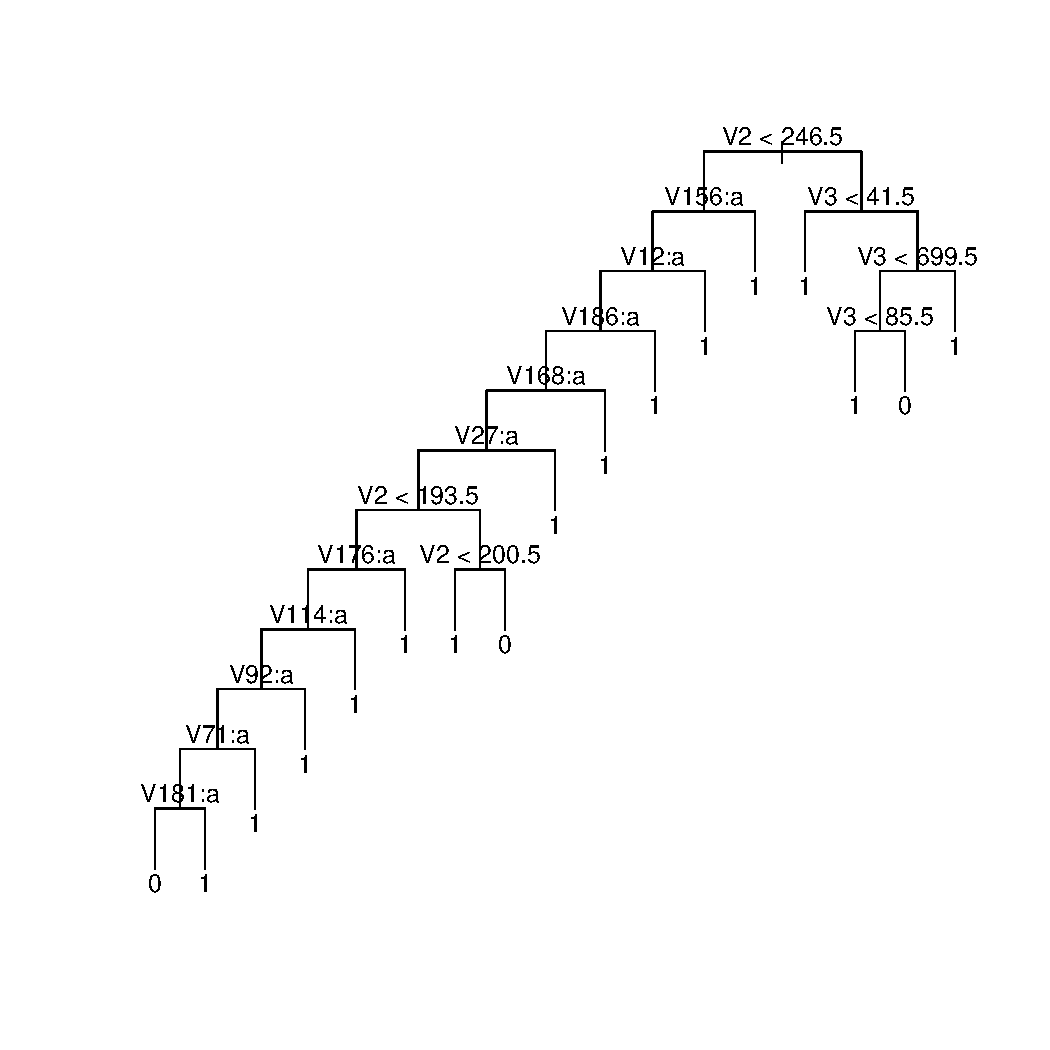
\includegraphics[scale=0.4]{ad_tree.pdf}
  \caption[The greedy algorithm tree for the internet ads dataset]{The greedy tree.}\label{fig:ads_image1}
\endminipage\hfill
\minipage{0.35\textwidth}
  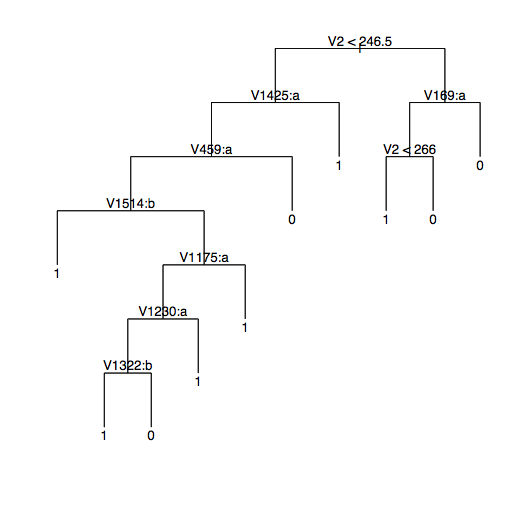
\includegraphics[scale=0.4]{CGM.png}
  \caption[The CGM algorithm tree for the internet ads dataset]{The tree found by the CGM algorithm on the internet ads dataset.}\label{fig:ads_image2}
\endminipage\hfill
\end{figure}
\begin{figure}
\minipage{0.35\textwidth}%
  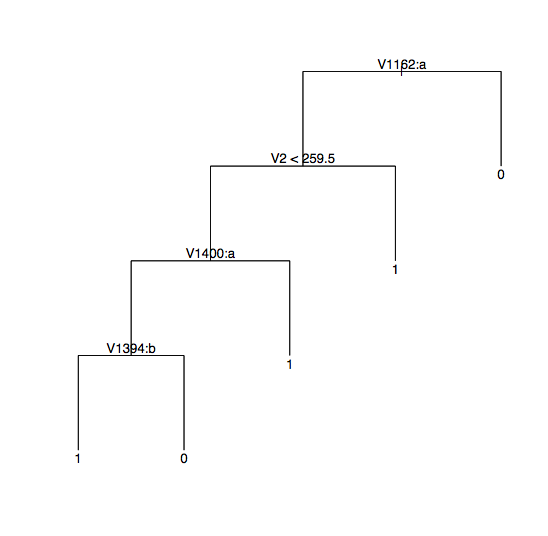
\includegraphics[scale=0.4]{estim2_tree.png}
  \caption[The weighted method tree for the internet ads dataset]{Best tree using the weighted method on the internet ads dataset.}\label{fig:ads_image3}
\endminipage\hfill
\minipage{0.35\textwidth}%
  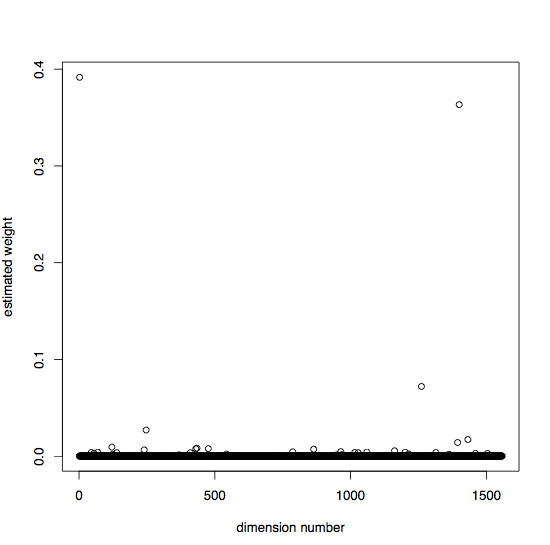
\includegraphics[scale=0.4]{weights_estim2.png}
  \caption[Estimated covariate weights for the internet ads dataset]{Estimated covariate weights using the internet ads dataset.}\label{fig:ads_image4}
\label{fig:uci_cov_weights}
\endminipage
\end{figure}
\begin{table}[h]\footnotesize
\centering
  \begin{tabular}{| c | c | c }
  \hline 
Method & Misclass Prob.\\
      \hline 
Greedy & 5.578\% \\ %0.0557598      \\
 CGM &   7.2\% \\%.0716912   \\
   Weighted & 5.598\% \\%0.0559853   \\
      \hline
  \end{tabular}
    \caption[Misclassification probabilities for internet ads dataset]{Misclassification probabilities of the three tree fitting methods on the internet ads dataset.}
      \label{tab:misclass_uci}
\centering
\end{table}

% latex table generated in R 2.15.0 by xtable 1.7-0 package
% Thu Feb 21 12:06:56 2013

\begin{table}[ht]
\hspace{-.7in}
\begin{tabular}{r|rrrrrrrrrrrrrrrrrrrrrrrrrrrrrrrrrrrr}
  \hline
 Cov Num & 2$^*$ & 1400$^*$ & 1261 & 247 & 1432 & 1394$^*$ & 121 & 434 & 476 & 430 & 864 & 240 \\
 Rank & 607.78$^*$ & 563.94$^*$ & 111.91 & 42.00 & 26.78 & 21.99$^*$ & 14.66 & 12.97 & 12.12 & 11.84 & 11.28 & 10.15 \\
 \hline
Cov Num & 1162$^*$ & 964 & 787 & 1060 & 69 & 1201 & 45 & 1015 & 1314 & 139 & 410 & 1028 \\ 
 Rank   & 8.74$^*$ & 7.33 & 7.05 & 6.77 & 6.48 & 6.48 & 5.92 & 5.92 & 5.92 & 5.64 & 5.64 & 5.64\\
 \hline
 Cov Num& 55 & 1460 & 1504 & 1214 & 543 & 123 & 1362 & 967 & 368 & 949 & 253 & 813 \\ 
  Rank   & 4.79 & 4.51 & 4.51 & 3.66 & 3.38 & 3.10 & 3.10 & 2.54 & 2.26 & 2.26 & 1.41 & 1.13 \\ 
   \hline
\end{tabular}
\caption[The set $J$ of covariates using Equation \ref{eqn:cov_inclusion_rule}]{The set $J$ of possibly included covariates from Equation \ref{eqn:cov_inclusion_rule}. Covariates are listed in decreasing order of the value used to include them in $J$. Stars indicate covariates used in Figure \ref{fig:ads_image3}. The rank is a numeric value that follows from Equation \ref{eqn:cov_inclusion_rule}.  }
\label{tab:ads_data_ranks}

\end{table}

The best tree is fit using our weighted method. The tree is best both in terms of simplicity, and in terms of misclassification probabilities, see Table \ref{tab:misclass_uci}. The CGM approach is not as good at predicting as those trees found by either the greedy or our weighted approach. Amongst the weighted and greedy approaches, the tree found by the greedy algorithm is far more complex than the tree found by our weighted method. The weighted method is essentially as good in terms of prediction error as the greedy method and is simpler to understand and interpret. Moreover, the greedy method and the CGM method do not provide output explicitly indicating which covariates are useful in the model.

Figure \ref{fig:uci_cov_weights} presents the estimated  probability of selection from our model. In this case there are three covariates that are clearly important in the model. The covariates selected according to the rule from Equation \ref{eqn:cov_inclusion_rule} are listed in decreasing order in Table \ref{tab:ads_data_ranks}. The covariates used in the tree in Figure \ref{fig:ads_image3} correspond to a subset of these covariates and are starred in the table. The starred covariates are: the width of the image, the url tag ``tkaine+bars'', the url tag ``www.irish-times.com'', and the url tag ``click''. The tag ``click'' is not particularly surprising because many ads are in the form of images that pop up a secondary webpage if you click on the image. The ``Irish Times'' is a newspaper and a perusal of their current webpage indicates that they have many images that accompany news articles and we can reasonable assume the website was similar when the dataset was created. The width field is also not surprising, wide windows facilitate better views of images. It is not very clear what the field ``tkaine+bars'' means. Perhaps some of the images come from a collection of webpages during Tim Kaine's race for mayor of Richmond, Virginia, in 1998. Admittedly, more information on this field would be desirable. 
 
\subsection{Discussion of Results}\label{sec:conc}
In this chapter we studied the application of MCMC data partitioning models to large dimensional data. We showed that, in large dimensional data sets, the methods used on low dimensional examples will not work effectively. We provided a simple modification that greatly improves the accuracy and utility of the partitioning scheme in large dimensional datasets. 

 When running MCMC algorithms on large dimensional data,we spend more time searching the covariates that are important (high probability) and ignoring the covariates that are not useful (the low probability ones). Moreover, the values of the probabilities for each covariate are on a probability scale providing intuitive interpretation of the values sampled from the posterior distribution of weights.
Sparsifying our tree search procedure provides us with several benefits. Firstly, we are able to separate the covariates into groups of high and low probability. Secondly, this gives us simplified interpretation of the tree models by searching for simple trees and eases inference for the analyst. Thirdly, we explore the state space more efficiently than the nonsparse greedy approach or the CGM search approach. 

Finally, we note that our approach to sparsity is different from the approach in Chipman, George and McCulloch \cite{chipman2000hierarchical}. In their work the goal was to model using short trees, so sparsity was achieved as a byproduct of constraining the complexity of the decision tree. Furthermore, a simple tree was their primary goal and no measure of usefulness on each covariate was desired. The inferential difficulties of the pruning rule noted in the introduction still apply to the Chipman et al. \cite{chipman2000hierarchical} method, whereas our dimension weighting does not have this difficulty. 

%\subsubsection*{Acknowledgements}
%We would like to thank Dr. Robert Gramacy for clarification of several aspects of his papers and for the referees for their comments which improved on an early draft of this paper. 
%\subsubsection*{References}



%% Chapter(s) on ALoVaS method

\section{Additive Logistic Variable Selection: The ALoVaS method}

\subsection{Normal Distributions Transformed to the Unit Simplex: ALT and ALN Dynamics. }\label{sec:ALN_chapter}

This chapter outlines the additive logistic transformation, which transforms a $d$ dimensional multivariate normal distribution onto the unit simplex in $d+1$ dimensions. Note that the unit simplex in $d+1$ dimensions actually lies in a subspace of $d$ dimensions because of the constraint that the sum of the probabilities equals one. 

The goal of this chapter is to find a transform that moves the space $\mathbb{R}^d$ \newnot{symbol:real} to the simplex $\mathbb{S}^d$. \newnot{symbol:simp} The simplex $\mathbb{S}^d$ is a space defined by the constraints $\{x_i: 0<x_i<1, \sum_{j=1}^dx_j <1 \}$, and the extra term $x_{d+1}=1-\sum_{j=1}^d x_j$ ensures the total sums to 1.  

Define the notation $\yvec$, for the normal random variables that reside in the $\Rsp{d}$  dimensional space. Define the notation $\xvec$  for the vector that resides on $\simp{d}$, the simplex in $d$ dimensions. We use an underline to indicate that the stated quantity is a column vector and capital greek letters (and $I$) will denote matrices (the identity matrix) 

\begin{equation}\label{eqn:simplex_transform}
x_i = \frac{e^{y_i}}{1+\displaystyle{\sum_{j=1}^de^{y_j}}}. \\
\end{equation}
Define the Jacobian of the transformation as
\newnot{symbol:jacobian}
\begin{equation}\label{eqn:jacobian}
J(\yvec \vert \xvec) = \left( \prod_{j=1}^{d+1}x_j \right)^{-1}.
\end{equation}

It is important to note that $\yvec\in\Rsp{d}$, whereas $\xvec\in\simp{d}$. The $d$ dimensional normal has the usual parameters and density

\begin{equation}\label{eqn:multinormal}
f_{\yvec}(\yvec\vert \Sigma, \mu)=(2\pi)^{-d/2}|\Sigma|^{-1/2}\exp{\left(-1/2(\yvec-\muvec)^T\Sigma^{-1}(\yvec-\muvec)\right)}.
\end{equation}

Upon applying the transformation defined by Equation \ref{eqn:simplex_transform}, we arrive at the additive logistic normal (ALN) distribution, with density 

\begin{equation}
f_{\xvec}(\xvec\vert \Sigma, \mu)=\frac{(2\pi)^{-d/2}}{\sqrt{\vert\Sigma\vert}\prod_{j=1}^{d+1}x_j } 
\exp{\left(-1/2(\text{log}(\xvec_{(d+1)}/x_{d+1})-\muvec)^T\Sigma^{-1}(\text{log}(\xvec_{(d+1)}/x_{d+1})-\muvec)\right)}.
\end{equation}
The vector notation $\xvec_{(d+1)}$ denotes the vector in $d$ dimensions that has the $d+1$ entry removed from the vector $\xvec$. 
It is important to note that this density function is defined on the space $\simp{d}$ and \emph{not} on the space $\Rsp{d}$. 

A useful property of this transform is that we can handle probabilities defined on the $d$ dimensional simplex while working with a normal distribution. This is a common and comfortable probability distribution for most statisticians and applied scientists.
We now wish to understand how the specification of the mean vector $\muvec$ and the covariance matrix $\Sigma$ impact the structure of the ALN density. From simulation we can formulate the following conclusions: 

\begin{itemize}
\item With $\Sigma=I$, increasing the mean vector in the positive direction in any one of the $d$ components individually corresponds to shifting density towards the corner of the simplex associated with that covariate. 
\item With $\Sigma=I$, increasing the mean vector in the negative in \emph{all} $d$ components corresponds to shifting density towards the $d+1$ corner of the simplex. 
\item Keeping $\muvec =\vec{0}$, adjusting any of the variances corresponds to shifting towards a projected space of $\simp{d}$. 
\item With $\muvec =\vec{0}$, making one variance small corresponds to the shifting density towards the median of the simplex associated with the remaining $d$ dimensions. 
\item Making the $\Sigma$ matrix approximately singular and moving $\muvec$ in the negative direction for all components places most of the probability density along the median of simplex associated with first $d$ dimensions. 
\item If $\Sigma = \text{Diag}(\sigma^2_j)$,\newnot{symbol:diag} as the $\sigma^2_j$ entries become smaller, the probabilities approach the CGM specification.    
\end{itemize}

The ALN density can be simulated using the transformation defined in Equation \ref{eqn:simplex_transform} and the fact that it is easy to simulate from the vector normal distribution. 

\begin{figure}[ht]
\begin{minipage}[b]{0.45\linewidth}
\centering
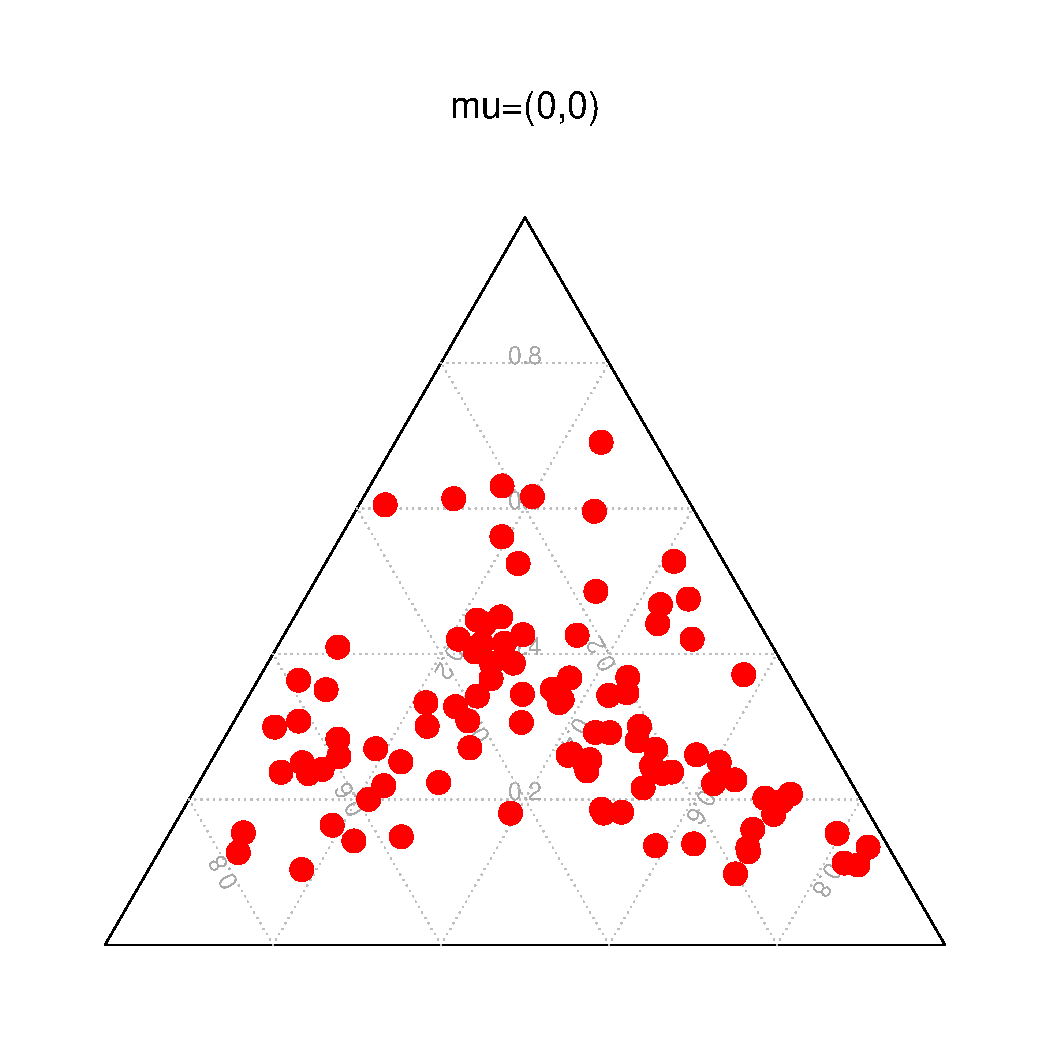
\includegraphics[width=\textwidth]{mu0_0.pdf}
\caption[ALN plot with a zero mean vector]{In this figure, $\muvec$ has all zero entries, with $\Sigma=I$, corresponding to the equiprobable case. Each probability is approximately $1/(d+1)$. }
\label{fig:figure9}
\end{minipage}
\hspace{0.5cm}
\begin{minipage}[b]{0.45\linewidth}
\centering
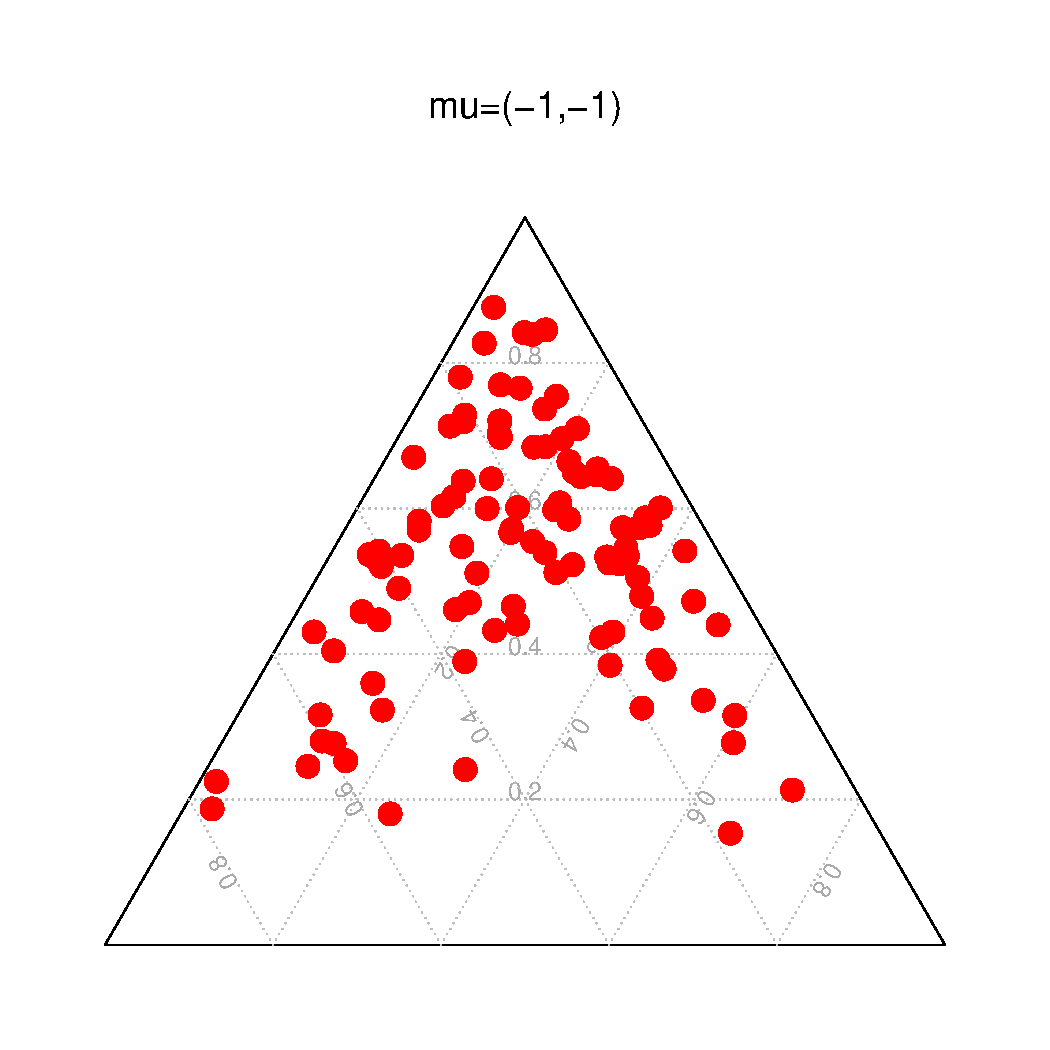
\includegraphics[width=\textwidth]{mu-1-1.pdf}
\caption[ALN plot with a negative one mean vector]{In this figure, $\vec{\mu}=(-1,-1)^T$, with $\Sigma=I$, corresponds to moving towards a sparser set of covariates. }
\label{fig:figure10}
\end{minipage}
\end{figure}

\begin{figure}[ht]
\begin{minipage}[b]{0.45\linewidth}
\centering
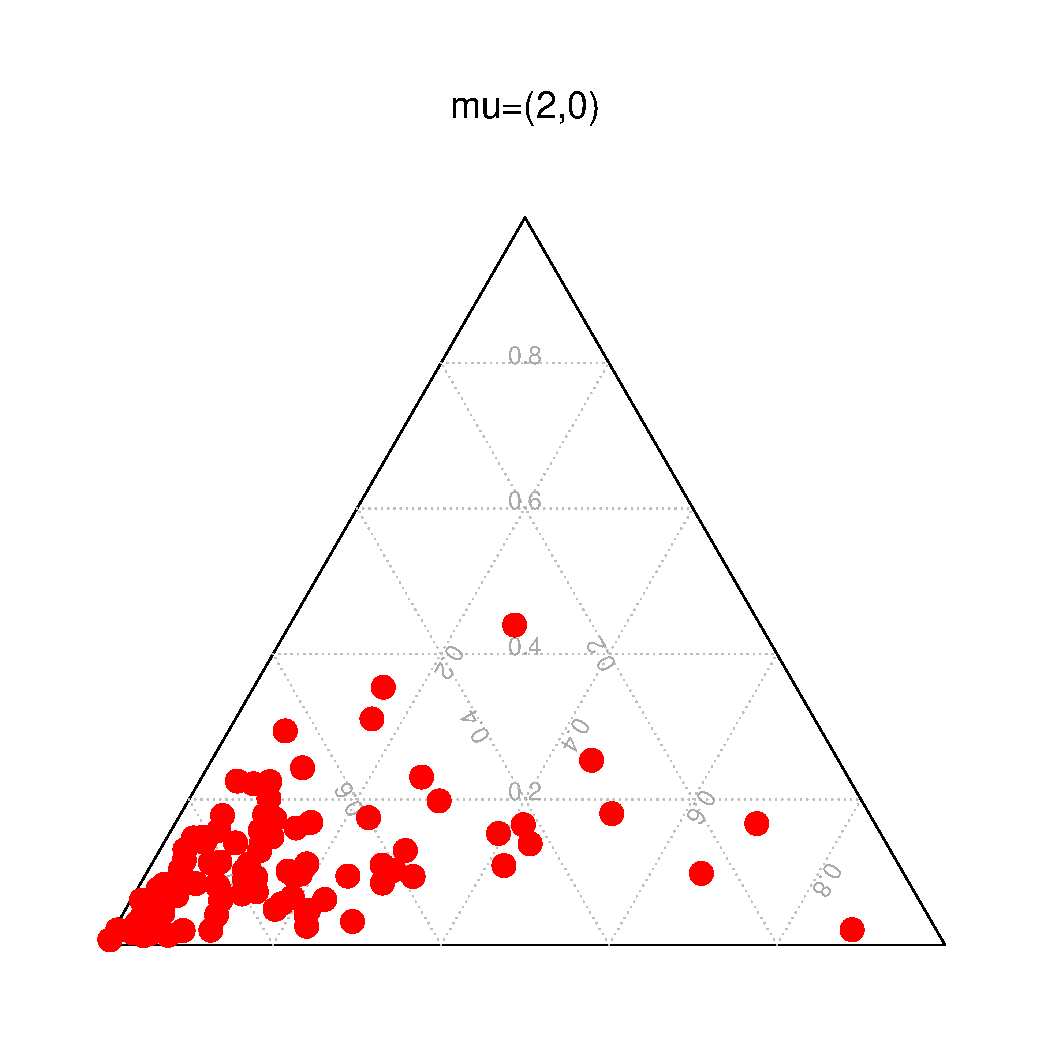
\includegraphics[width=\textwidth]{mu2_0.pdf}
\caption[ALN plot with a mean vector $(2,0)^{T}$]{$\vec{\mu}=(2,0)^T$, with $\Sigma=I$, moves the density towards one corner of the simplex. }
\label{fig:figure1}
\end{minipage}
\hspace{0.5cm}
\begin{minipage}[b]{0.45\linewidth}
\centering
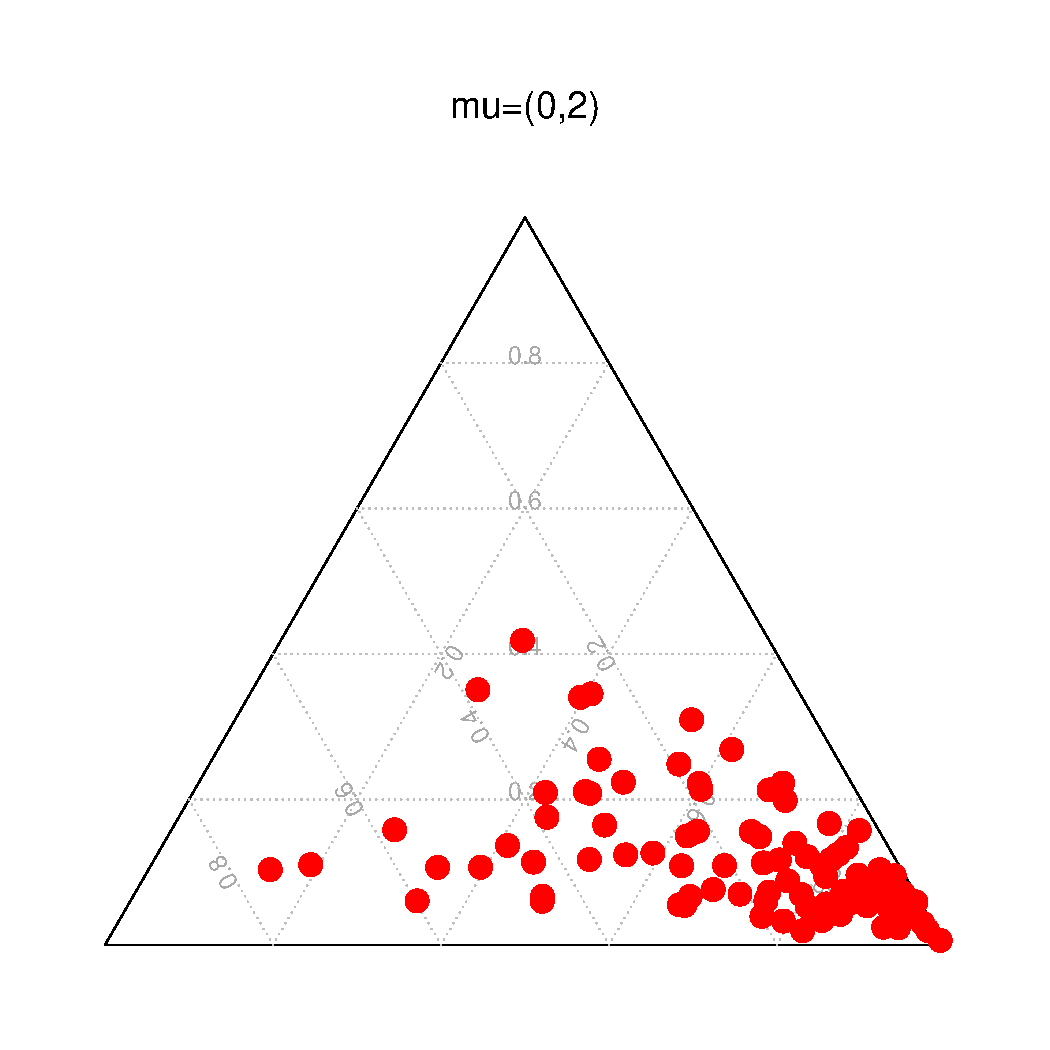
\includegraphics[width=\textwidth]{mu0_2.pdf}
\caption[ALN plot with mean vector $(2,0)^{T}$]{$\vec{\mu}=(0,2)^T$, with $\Sigma=I$, moves the density towards the other corner of the simplex. }
\label{fig:figur2}
\end{minipage}
\end{figure}

\begin{figure}[ht]
\begin{minipage}[b]{0.45\linewidth}
\centering
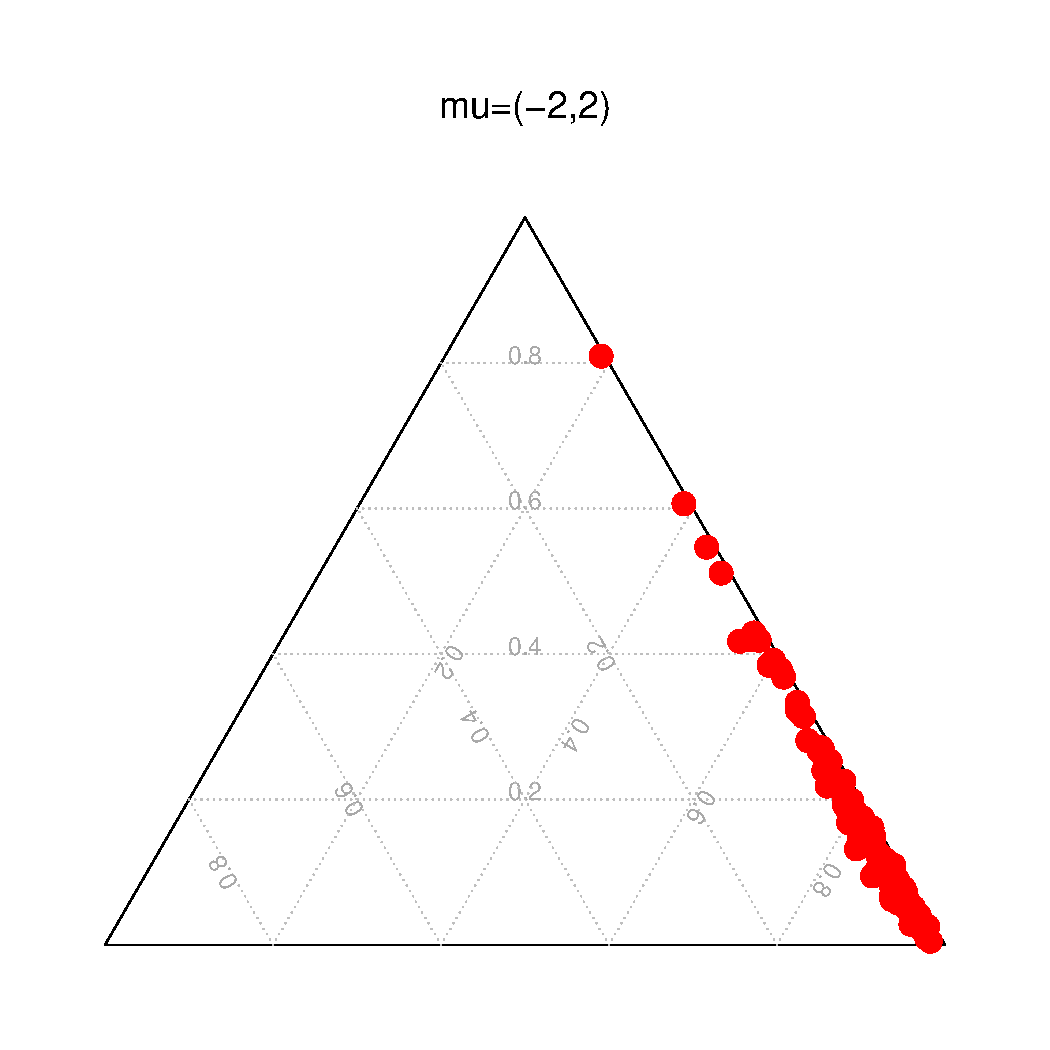
\includegraphics[width=\textwidth]{mu-2_2.pdf}
\caption[ALN plot with a mean vector of $(-2,2)^{T}$]{$\vec{\mu}=(-2,2)^T$, with $\Sigma=I$, corresponds to most probability mass along a corner of the simplex and is a sparse representation.} 
\label{fig:figure3}
\end{minipage}
\hspace{0.5cm}
\begin{minipage}[b]{0.45\linewidth}
\centering
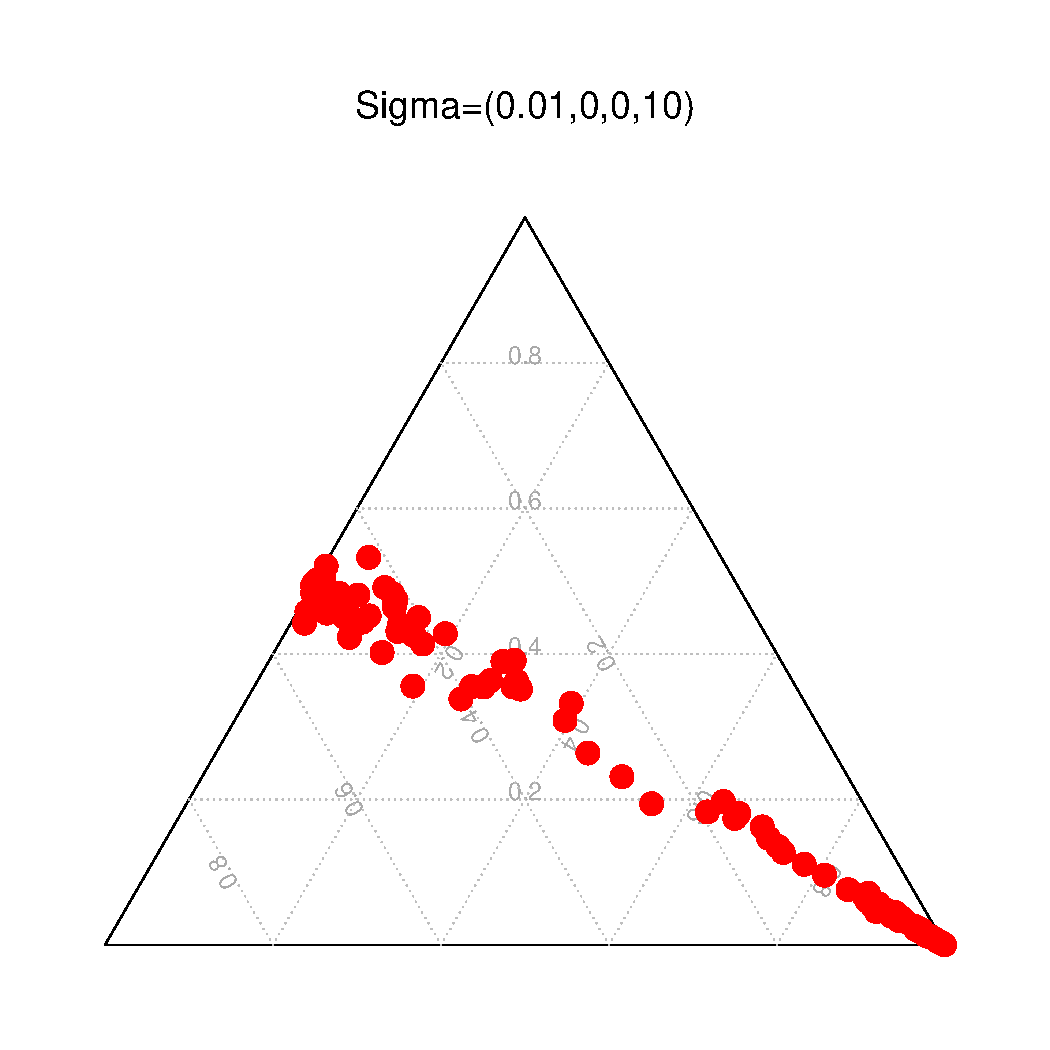
\includegraphics[width=\textwidth]{Sigma0_01_10.pdf}
\caption[ALN plot $\Sigma=\text{Diag(0.01,100)}$]{ $\vec{\mu}=\vec{0}$, with
 $\Sigma= \text{diag}(0.01, 100)$, corresponds to most density lying on a one dimensional subspace (the second covariate in the $\Rsp\ $ space).  }
\label{fig:figure4}
\end{minipage}
\end{figure}


\begin{figure}[ht]
\begin{minipage}[b]{0.45\linewidth}
\centering
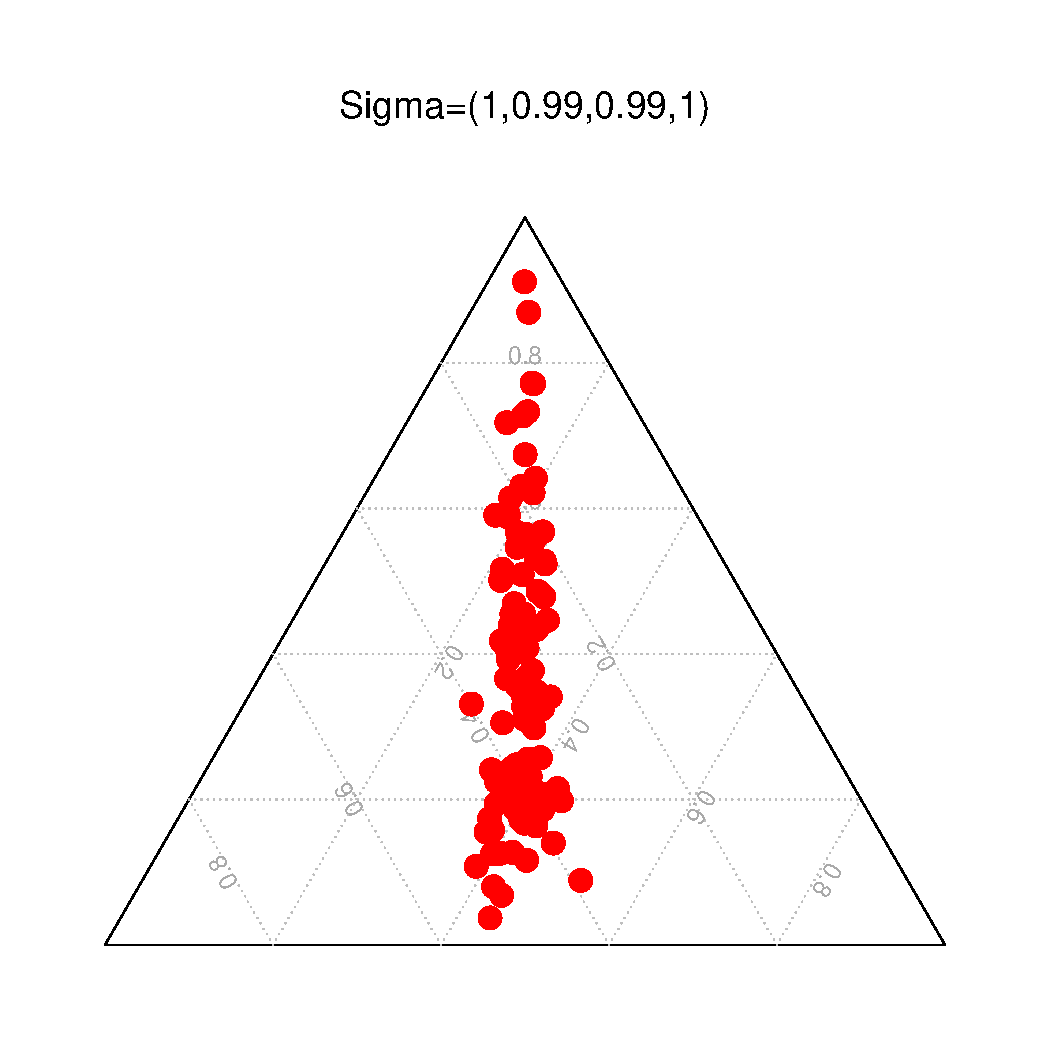
\includegraphics[width=\textwidth]{Sigma1_9_9_1.pdf}
\caption[ALN plot $\Sigma$ numerically singular]{Here $\Sigma$ is approximately singular and most of the probability mass in concentrated along the $d+1$th dimension in the $\mathbb{R}^{d+1}$ space.  }
\label{fig:figure5}
\end{minipage}
\hspace{0.5cm}
\begin{minipage}[b]{0.45\linewidth}
\centering
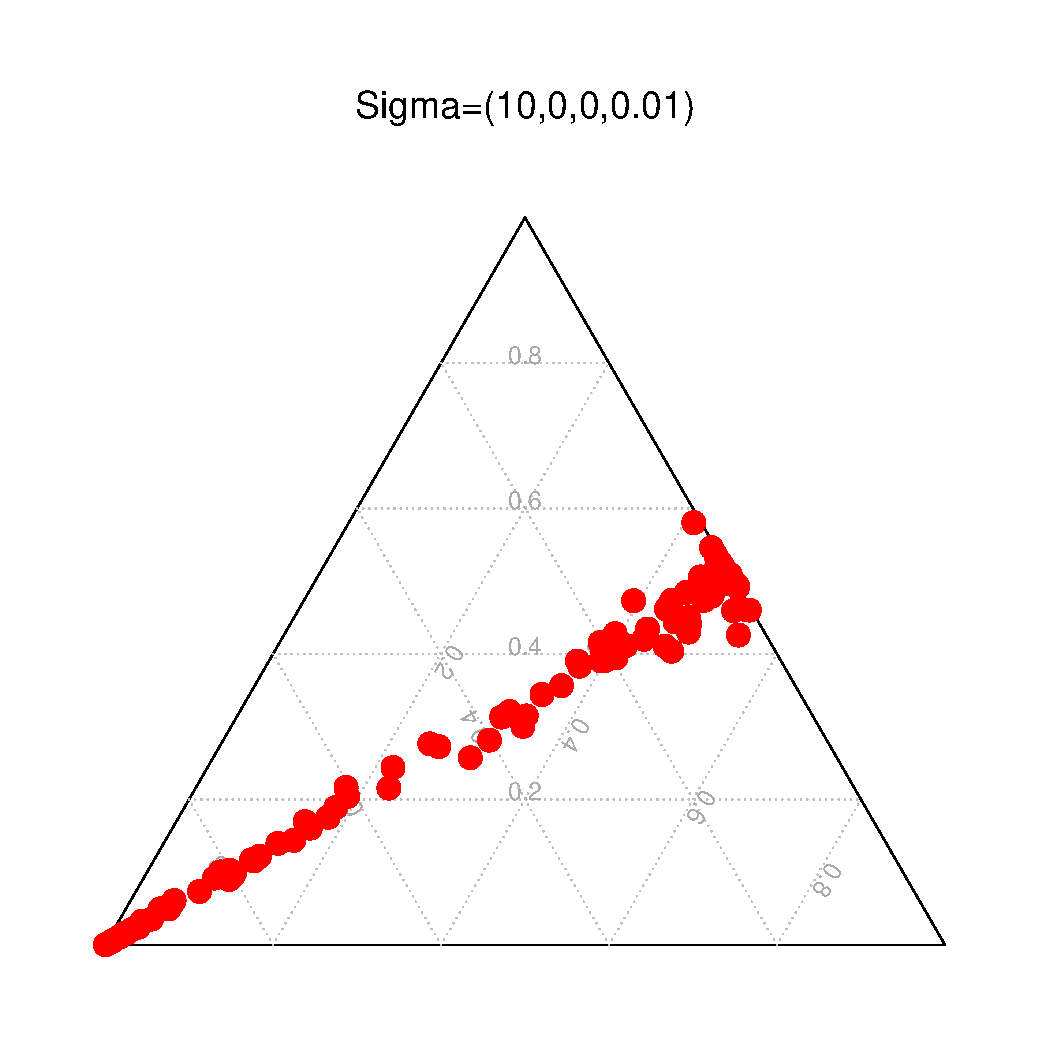
\includegraphics[width=\textwidth]{Sigma10_0_01.pdf}
\caption[Similar to the case in Figure \ref{fig:figure4} but with the variances reversed]{Similar to the case in Figure \ref{fig:figure4} but with the variances reversed.}
\label{fig:figure6}
\end{minipage}
\end{figure}

 \begin{figure}[ht]
\begin{minipage}[b]{0.45\linewidth}
\centering
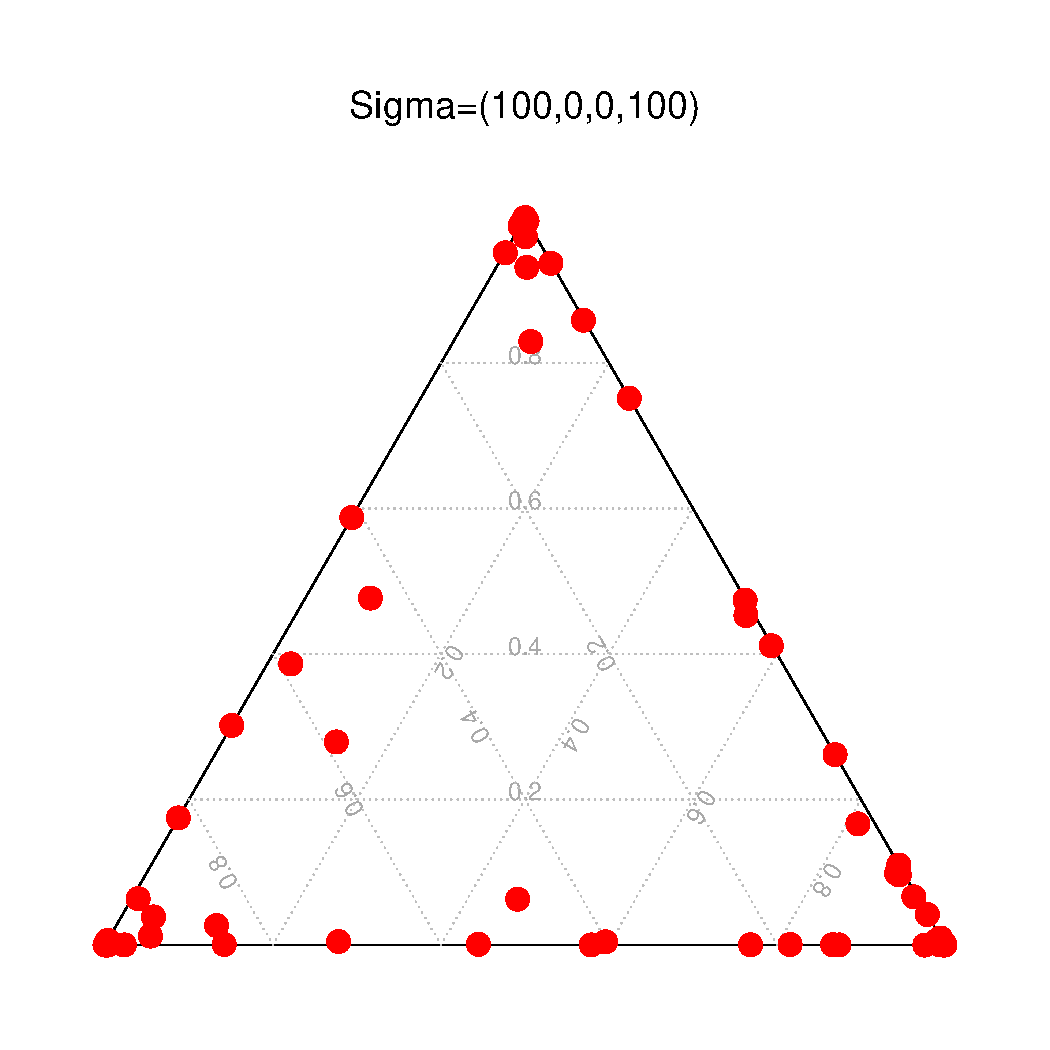
\includegraphics[width=\textwidth]{Sigma100_100.pdf}
\caption[ALN plot with a zero vector mean and $\Sigma=\text{Diag}(100,100)$]{$\vec{\mu}=\vec{0}$, with
 $\Sigma= \text{diag}(100, 100)$, corresponds to encouraging sparse representations \emph{a priori}.  }
\label{fig:figure7}
\end{minipage}
\hspace{0.5cm}
\begin{minipage}[b]{0.45\linewidth}
\centering
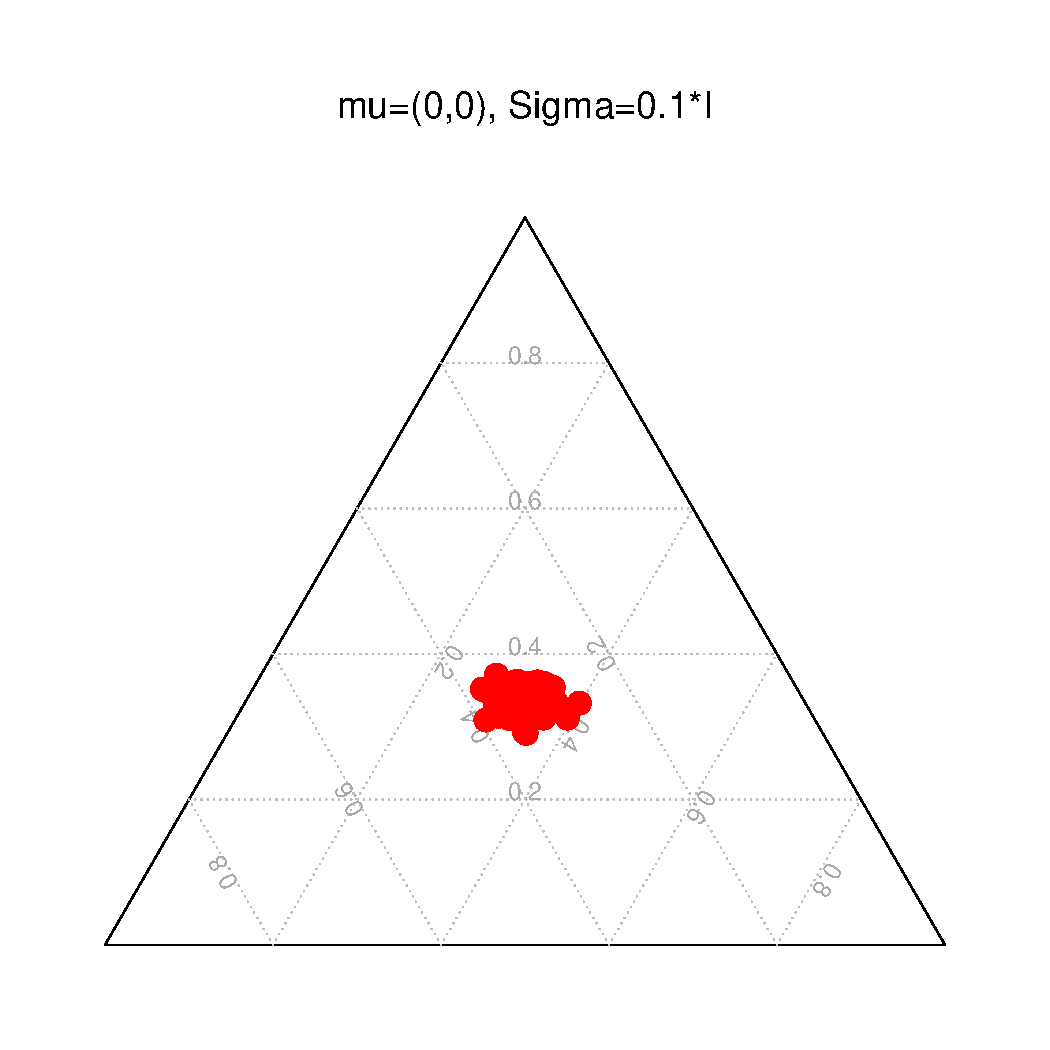
\includegraphics[width=\textwidth]{Sigma01_01.pdf}
\caption[ALN plot approximating the CGM model]{Here $\Sigma=0.1I$, and $\muvec=\vec{0}$, corresponds to roughly the CGM specification.}
\label{fig:figure8}
\end{minipage}
\end{figure}

 The simulations indicate that we can scale everything at approximately an $\mathcal{O}(d)$\newnot{symbol:big_oh} rate because of the diagonality of the variance covariance matrix, and no matrix inversions are required. The step that remains is to link this portion of the model with the (currently) observed data in the tree, so that better trees are favored over trees that are worse, when each is observed in the Markov chain. We will first work in the space $\Rsp{d}$ and then translate to probabilities by using Equation \ref{eqn:simplex_transform}.  
 
 If we focus on the means and a collection of variances in a multivariate normal i.i.d. model, then we must fully specify the likelihood and the prior to form our posterior. 
 
We define the likelihood of the tree by counting the tree's selected covariates and summing across all observed splits. The counting leads to the likelihood taking on discrete values for the observed data. Let us define a multiplier that can take on an arbitrary positive or negative value in a compact region. We then multiply the counts of splits on each covariate by this quantity, effectively creating a mean which can take arbitrary values in $\Rsp{}$. 

\subsection{A Simple Sampler Approach}

This subsection derives the full conditional densities for each necessary update in the Gibbs loop to sample posterior weights on each dimension in the CGM decision tree sampler. 
 Throughout this subsection we will use the notation $\odot$\newnot{symbol:hadamard} to denote a Hadamard product of two matrices or vectors. 
 
 \subsubsection{The General Strategy}
 There are many problems with using a Dirichlet prior and a Multinomial conjugate likelihood. The two most glaring problems are the implicit prior assumption of same scales on each covariate and the fact that all covariances or, equivalently, correlations must be negative. If the generative model of the data is a linear model with an interaction term and a decision tree model is fit to the data, then several splits will occur on the two interacting covariates. These splits will occur alternately until the curvature is sufficiently approximated \cite{ishwaran2010high}. This situation indicates a positive correlation between the two covariates. Higher order interactions will result in similar positive correlations between collections of covariates. Therefore we conclude the Dirichlet density as a posterior for the probability of selecting a covariate is an inferior model. Moreover, the initial motivation for modeling data with a decision tree was to handle survey data that contained many complex interactions that would be too computationally expensive to evaluate using linear model methods \cite{morgan1963problems}. 
 
 The likelihood will be denoted by
 
 \begin{equation}\newnot{symbol:mvn}
 MVN(\vec{c}\odot\vec{s}\vert \vec{\mu}, \Sigma=\text{Diag}(\sigma^2_j)).
 \end{equation}
 
 The prior is also a normal 
 
 \begin{equation}
 \pi(\vec{\mu}\vert \vec{\mu}_p, \Sigma)=MVN(\vec{\mu}\vert \vec{\mu}_p, \Sigma).
 \end{equation}

The priors on the variances are \iid $\sim \invgam{\sigma_j^2}{a_j}{b_j}$.
Finally the priors on the $c_j$s are \iid\ scaled beta's with densities 

\begin{equation}\newnot{symbol:scaled_beta}
S\beta(c_j\vert \alpha_j, \beta_j, -a, a)\equiv\pi(c_j\vert \alpha_j, \beta_j, -a, a)= \frac{(c_j+a)^{\alpha_j-1}(a-c_j)^{\beta_j-1}\Gamma(\alpha_j+\beta_j)}{(2a)^{\alpha_j+\beta_j-1}\Gamma(\alpha_j)\Gamma(\beta_j)}.
\end{equation}

A special case of these scaled beta densities is when $\alpha_j=\beta_j=1$, which yields uniform r.v.'s on the region  $[-a,a]$. 
For each $j=1, \dots, d$, we first calculate $s_j = \epsilon+\sum_{\forall \eta \in \mathcal{T}}\mathds{1}[\text{split on covariate j at node $\eta$}]$, for some fixed $\epsilon>0$.
Through basic Bayesian calculations we find that the full conditional distributionss are 

\begin{equation}
\pi(c_j\vert \mu_j, \sigma_j^2, a) \sim N_{[-a,a]}(c_js_j\vert \mu_j, \sigma^2_j) \text{(a normal truncated to the region $(-a,a)$),}
\end{equation}

\begin{equation}
\pi(\sigma^2_j \vert \mu_j, c_j, a) \sim \invgam{\sigma_j^2}{2a_j+2}{\frac{(c_js_j-\mu_j)^2+ (\mu_j-\mu_j^p)^2+b_j}{2}}, \text{ and } 
\end{equation}

\begin{equation}
\pi(\mu_j\vert \mu_j^p, c_j, \sigma^2_j)\sim N[c_js_j+\mu_j^p, \sigma_j^2].
\end{equation}

\subsection{Slice Sampling Gibbs Updates}

Ideally we would like everything to be a Gibbs step. This can be accomplished numerically using numerical approximations to the cumulative density of the standard normal distribution, here denoted $\Phi$, and $\Phi^{-1}$, the quantile function of the standard normal cumulative density. \newnot{symbol:sncdf} However, we can accomplish this directly using the technique of parameter expansion set forth in Damien and Walker \cite{damien2001sampling}, which we review here for completeness. 
 
We begin with the joint density of two random variables 

\begin{equation}
f(x,y) \propto \mathds{1}[0, \exp{(-x^2/2)}](y).
\end{equation}
The marginal of $x$ is a standard normal density. Through elementary probability calculations we find 

\begin{equation}\newnot{symbol:unif}
f(y\vert X=x) \propto Unif(0, \exp{(-x^2/2)}),
\end{equation}
 and 
 
 \begin{equation}
f(x\vert Y=y) \propto Unif(-\sqrt{-2log(y)}, \sqrt{-2log(y)}).
\end{equation}
The region upon which $X$ is defined arises from the solution of the inequalities $\{0\leq y \leq \exp{(-x^2/2)} \} $ for $X$, which is a quadratic equation in $X$. Similarly, if we have a truncated distribution truncated to the region $[a,b]$, we write the joint density 
 
 \begin{equation}
 f(x,y)=Unif((0\leq y\leq \exp{(-x^2/2)})\times (a,b)).
 \end{equation}
 Solving the resulting system of inequalities leads to the set 
 
 \begin{equation}
 \{-\sqrt{-2log(y)}, \sqrt{-2log(y)} \} \cap \{a, b\},
 \end{equation}
which results in the region for $x$

\begin{equation}
 \{\text{max}(a,-\sqrt{-2log(y)}), \text{min}(b,\sqrt{-2log(y)} )\} .
 \end{equation}
 Simulating from a truncated normal is equivalent to simulating from two uniforms on the appropriate regions and evaluating a natural logarithm and a square root function at each iteration. 
 
 A special case of these scaled beta densities is when $\alpha_j=\beta_j=1$, which yields uniform random variables on the region $[-a,a]$. 
For each $j=1, \dots, d$, we first calculate $s_j = \epsilon+\sum_{\forall \eta \in \mathcal{T}}\mathds{1}[\text{split on covariate j at node $\eta$}]$, for some fixed $\epsilon>0$.
Through basic Bayesian calculations we find the full conditionals in closed form
 
\begin{equation}\label{eqn:u_given_cjsj}
\pi(u \vert c_js_j, \mu_j, \sigma_j^2)= \text{Unif}(0, \exp{(\frac{-(c_js_j-\mu_j)^2}{2\sigma_j^2} )}),
\end{equation}

\begin{equation}
\pi(c_j \vert u) = \text{Unif}(\text{max}(-a,-\sqrt{-2log(u)}), \text{min}(a,\sqrt{-2log(u)} )),
\end{equation}

\begin{equation}
\pi(\sigma^2_j \vert \mu_j, c_j, a) \sim \invgam{\sigma_j^2}{2a_j+2}{\frac{(c_js_j-\mu_j)^2+ (\mu_j-\mu_j^p)^2+b_j}{2}}, \text{ and}
\end{equation}

\begin{equation}\label{eqn:muj_given_cj}
\pi(\mu_j\vert \mu_j^p, c_j, \sigma^2_j)\sim N[c_js_j+\mu_j^p, \sigma_j^2].
\end{equation}

 The Gibbs sampling step, nested within the MH sampler, proceeds by sampling from Equations \ref{eqn:u_given_cjsj}-\ref{eqn:muj_given_cj}.
At each iteration, once samples are drawn in sequence from the distributions given in Equations \ref{eqn:u_given_cjsj}- \ref{eqn:muj_given_cj}, we take the posterior samples of $\mu_j$ and transform these onto the $[0,1]$ scale, by using the ALN transform given in Equation \ref{eqn:simplex_transform}. 

We show results from a preliminary coding of the stated algorithm. We use two specificications for the prior means $\vec{\mu}^p$. One specification uses  $\vec{\mu}^p = \vec{0}$ (Figure \ref{fig:simple_sampler2}) and another uses $\vec{\mu}^p=(-2,-2,2,\dots,2)$ (Figure \ref{fig:simple_sampler1}). The difference in the results of sampled weights indicates that, if we can move from a negative to a positive value for the prior mean, we can greatly influence the selection of covariates. The graphic of posterior weights shown in Figure \ref{fig:simple_sampler1} is the correct set of weights for the data. 


%%%% -------Graphics from preliminary simulations using the simple sampler approach

 \begin{figure}[ht]
\begin{minipage}[b]{0.45\linewidth}
\centering
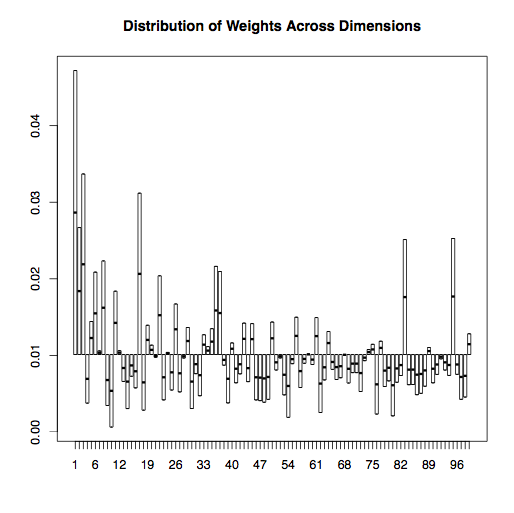
\includegraphics[scale=0.4]{simple_sampler2.png}
\caption[Results for the zero mean prior]{A zero mean prior. Note that the two covariates that should have large probabilities are covariates 1 and 2.}
\label{fig:simple_sampler2}
\end{minipage}
\hspace{0.5cm}
\begin{minipage}[b]{0.45\linewidth}
\centering
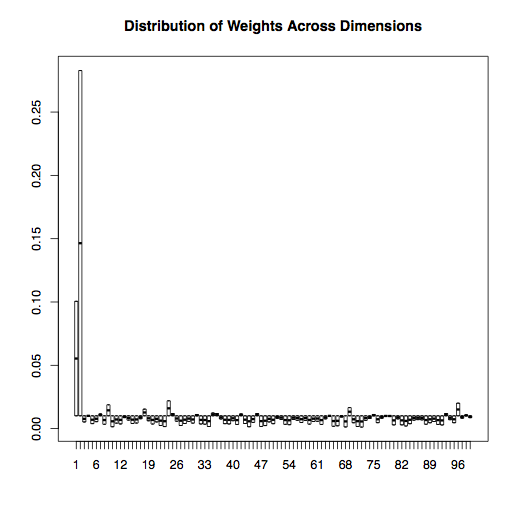
\includegraphics[scale=0.4]{simple_sampler1.png}
\caption[Results for the informative prior]{An informative prior. The first two prior means are 2 and the remaining prior means are set at -2.}
\label{fig:simple_sampler1}
\end{minipage}
\end{figure}


%%%%---------END OF: Graphics from preliminary simulations using the simple sampler approach

\subsection{A Stochastic Search Variable Selection Approach}

Using the results of George and McCulloch we derive Gibbs updates for each of the parameters and have as a special case the approach of CGM if all the dimension indicators are selected to be the point masses at zero. In this case the ALN transform puts probability $1/(d+1)$ on each dimension. 


We investigate three priors for use in variable selection with decision trees. They are: 

\begin{itemize}
\item A stochastic search approach using method of George and McCulloch \cite{cui2008empirical,george1993variable}. 
\item A lasso prior on the means of the MVN, \newabbrev{abbrev:MVN} using parameter expansion to use Gibbs updates \cite{park2008bayesian}. 
\item A multivariate half-Cauchy prior using parameter expansion (Huang and Wand method) \cite{huang2013simple,polson2011half,carvalho2010horseshoe,carvalhohandling}. 
\end{itemize}

We will discuss the preliminary details of each method in sequence in this chapter. 

Variable selection with SSVS facilitates a Bayesian approach to variable selection in decision trees. Prior methods have examined bootstrapping approaches and used some complicated math to allow the statistician to peer inside the black box method known as randomForest \cite{ishwaran2010high, ishwaran2007variable}, often with little insight or understanding. The SSVS prior allows us to ``test'' whether the constant prior probability of selecting a covariate for all dimensions is appropriate for the given dataset. This means we can test, for any dataset, whether the CGM model of covariate selection is appropriate.

%We will implement and compare our method against other methods such as observed frequency, a na\"{i}ve method, as well as the maximal subtree approach of Ishwaran et al. \cite{ishwaran2010high, ishwaran2007variable}. The SSVS approach involves a prior on the normal means of the form 

\begin{equation}
\pi(\mu_i\vert \tau_i, p_i, c_i) \propto p_iN(\mu_i, \tau_i^2)+(1-p_i)N(\mu_i, \psi^2_i+\tau_i^2).
\end{equation}

Here the $\psi_i >0$ and the $\tau_i>0$. Usually $p_i\equiv1/2$ but it is also possible to put a prior on these hyper-parameters. The advantage of a mixture prior in this form is that Gibbs samples are readily available for each of the desired quantities facilitating fast sampling.     

\subsection{Parameter Expansions For the Lasso and Horseshoe Priors}
In this section we propose to use parameter expansion to facilitate Gibbs sampling within the sampling framework for the posterior means ($\mu_j$) for each covariate in the normal space. We use the ALN transform to convert the $\mu_j$ to probabilities using the ALT transform. 
We use the scale mixture of normals representation to write the Laplace prior is parameter expanded form. This representation is stated here for reference.

If $V \sim \text{Exponential(1)}$ and $Z \sim N(0, 1)$ independent of $V$, then $X = \mu + b \sqrt{2 V}Z \sim \mathrm{Laplace}(\mu,b)$. 

Equivalently we can write this as the hierarchy

\begin{equation}\label{eqn:normal_cond_lhood_lasso}
X \vert V \sim N[\mu, \sigma^22V],
\end{equation}

\begin{equation}\newnot{symbol:exponential_dist}
V \sim \text{Exponential}(1), \text{ and}
\end{equation}

\begin{equation}\newnot{symbol:laplace_dist}
X \sim \text{Laplace}(\mu, \sigma).
\end{equation}

What we want to examine here is whether shrinkage along an $L_1$ penalty will achieve similar results to the SSVS approach and give us meaningful results. The belief here is the same as in the SSVS approach, shrinkage will shrink means toward zero in the multivariate normal. These sampled values from the multivariate normal will then be transformed into something on the $[0,1]$ (probability) scale using the ALN transform. Values of zero, or near zero, on the normal space transform into values of approximately $1/(d+1)$. The probabilities with values around $1/(d+1)$ correspond to covariates we are indifferent about. A confounding aspect of interpreting the probabilities is that they must all sum to 1. Therefore if some values are excessively small this may push all the other probabilities to be larger. If something like this happens it is then difficult to determine which covariates are non-informative. Further simulations regarding selecting covariates using the rule of Equation \ref{eqn:cov_inclusion_rule} will be conducted using the ALN transform and will be done on several simulated and real data examples.    

The following result will be useful for parameter expansion. If 

$X\vert a \sim \mathrm{Inv\textendash Gamma}(\nu/2, \nu/a)$ and  $a \sim \mathrm{Inv\textendash Gamma}(1/2,A^2)$, then $\sqrt{X}\sim \mathrm{Half\textendash Cauchy}$. 

\begin{align*}
f(x) &= \int_0^\infty \underbrace{  \frac{\nu^{\nu/2}}{a^{\nu/2}\Gamma(\nu/2)x^{(\nu/2)+1}}\exp{(-\frac{\nu}{ax})}   }_{=f(x\vert a)} \underbrace{\frac{\exp{(-\frac{1}{aA^2})}}{A\sqrt{\pi}a^{3/2}}}_{=f(a)} da\\
&=\frac{\nu^{\nu/2}}{A\sqrt{\pi}\Gamma(\nu/2)x^{(\nu+2)/2}}\underbrace{\int_0^\infty a^{-\nu/2-1/2-1}\exp{(-(1/a)(\nu/x+1/A^2))}da}_{=\text{Inv-Gamma kernel}}\\
&=\frac{\nu^{\nu/2}\Gamma((\nu+1)/2)}{A\sqrt{\pi}\Gamma(\nu/2)x^{(\nu+2)/2}(\nu/x+1/A^2)^{(\nu+1)/2}}\\
&\propto \frac{1}{\sqrt{x}x^{(\nu+1)/2}(\nu/x+1/A^2)^{(\nu+1)/2}}\\
& =\frac{1}{\sqrt{x}(\nu+x/A^2)^{(\nu+1)/2}  }\\
&=\frac{1}{\sqrt{x}(\nu+x/A^2)^{(\nu+1)/2}  }.
\end{align*}

Making the change of variable $x=y^2$, which implies $dx/(2\sqrt{x})=dy$, shows us that 

\begin{equation}
f(y) \propto (1+(y/A)^2/\nu)^{-(\nu+1)/2},
\end{equation}
for $y>0$ which is the definition of a half-Cauchy density. 

Huang and Wand \cite{huang2013simple} indicate that using an inverse-Wishart prior on the variances, with each standard deviation having a half-Cauchy prior, gives a scaled beta marginal for each correlation. At this point it is worth recalling that the t and half-t distributions have as special cases, the Cauchy and half-Cauchy distributions when the degrees of freedom parameter ($\nu$) in the t and half-t is set to $\nu=1$. 



\section{The ALoVaS Model}\label{sec:Introduction}
	
In this paper we describe a decision tree method to explicitly handle variable selection in high-dimensional data, called the Additive Logistic Variable Selection  (ALoVaS) method. This method allows us to reuse regularization approaches, prominent in the linear model literature, and apply them to decision trees. Although Bayesian methods have been available for use with decision trees since the seminal papers of Chipman, George, and McCulloch \cite{chipman1998bayesian}  and Denison, Mallick, and Smith \cite{denison1998bayesian}, there has been little work to alleviate the practical difficulties of applying Bayesian decision trees for high-dimensional data. A notable exception is the approach of Roberts and Leman \cite{Roberts:2013uq} who used a Dirichlet prior on the covariate selection probabilities. Also, the non-Bayesian approaches described by Ishwaran and coauthers \cite{ishwaran2011random,ishwaran2010high,ishwaran2007variable} deserve mentioning these authors use an initial bootstrap sample to determine the covariate selection probabilities and then use these estimated covariate selection probabilities in a subsequent random forest algorithm. Moreover, in the discussion of Chipman et al., it is noted by Knight, Kustra, and Tibshirani \cite{knight1998bayesian} that the Bayesian approach to decision trees breaks down as the number of covariates increases. 

In contrast to the literature on decision tree variable selection, the literature on variable selection for linear models is voluminous. Textbooks have been written on variable selection for linear models \cite{miller2002subset}. Each year several papers are published in major statistical journals developing properties of various variable selection methods and proposing modifications to improve known deficiencies. 

Let us start with the linear model
\begin{equation}\label{def:linear_model}
\vec{y} = X\vec{\mu} + \vec{\epsilon},
\end{equation}
where $\vec{\epsilon}$ is an $n \times 1$ vector of random errors, typically assumed to follow a multivariate normal distribution. Also, $X$ is an $n \times p$ matrix, also called the design matrix, which determines the mean value associated with each observed response, the associated element of the $n\times 1$ vector $\vec{y}$. It should be noted that in this section and throughout this paper we use the cell means model to describe the ANOVA linear model. Thus here $X$ denotes an incidence matrix of full rank. It is well known that if $n$, the number of observations, is less than $p$, the number of covariates, then the estimated values of the $\mu_j$, for $j=1,\dots,p$, denoted $\hat{\mu}_j$, are not estimable. However, regularizing, or equivalently putting a prior on the $\mu_j$, results in estimable values for the $\hat{\mu}_j$. Moreover, a nice property of the linear model is that covariates deemed not useful can have their coefficients coded as zero, whereas useful covariates can be encoded with non-zero coefficients. Thus, a sparse linear model indicates knowledge that certain covariates are not useful. Sparse linear models are typically necessary when dealing with high-dimensional data, especially in the $p>n$ case. 

The Additive Logistic Transform (\ALT), when employed with a multi-category logistic regression, is used as the canonical inverse link function \cite{mccullagh1989generalized}. The \ALT\ is referred to as the softmax function in the machine learning literature \cite{bishop2006pattern}. Additionally, the \ALT\ is fundamental to the analysis of compositional data \cite{aitchison1986statistical}. The \ALT\ is defined by the vector valued function given in Equation \ref{eqn:alt}, 
\begin{equation}\label{eqn:alt}
\vec{q} = \left[ q_1, q_2,\dots, q_{p-1}, q_p \right] =\vec{g}^{-1}(\vec{\mu})= \left[ \frac{e^{\mu_1}}{1+S_{p-1}},\frac{e^{\mu_2}}{1+S_{p-1}}, \dots,\frac{e^{\mu_{p-1}}}{1+S_{p-1}},\frac{1}{1+S_{p-1}} \right],\end{equation} 
where $S_{p-1}=\sum_{j=1}^{p-1}e^{\mu_j}$. Moreover, the \ALT\ is an invertible mapping from the $p$ dimensional real number system to a probability simplex. This allows us to calculate the distribution of the random variables obtained by the \ALT\ via a change of variables. In this paper we focus on the Additive Logistic Normal (\ALN) density, obtained by applying the \ALT\ to a random vector with a multivariate normal density. The \ALN\ density has proved successful in the correlated topic model \cite{blei2007correlated,lafferty2005correlated}.  Additionally, for our applications the \ALN\ density allows us to model covariate selection probabilities that have both positive and negative correlations, whereas distributions like the Dirichlet density only permit negative correlations.

By focusing on the \ALT, we are able to transform the decision tree variable selection problem into a problem of variable selection in a linear model. The upshot of this is that we may use variable selection methods, prevalent in the linear model literature, with decision trees. Thus, we can sample from a posterior distribution of the covariate selection probabilities and determine the utility of covariates, simultaneously performing variable selection and decision tree fitting. 
 
\begin{figure}[H]
  \centering
  \begin{tabular}{ccc}
 \subfigure[]
 {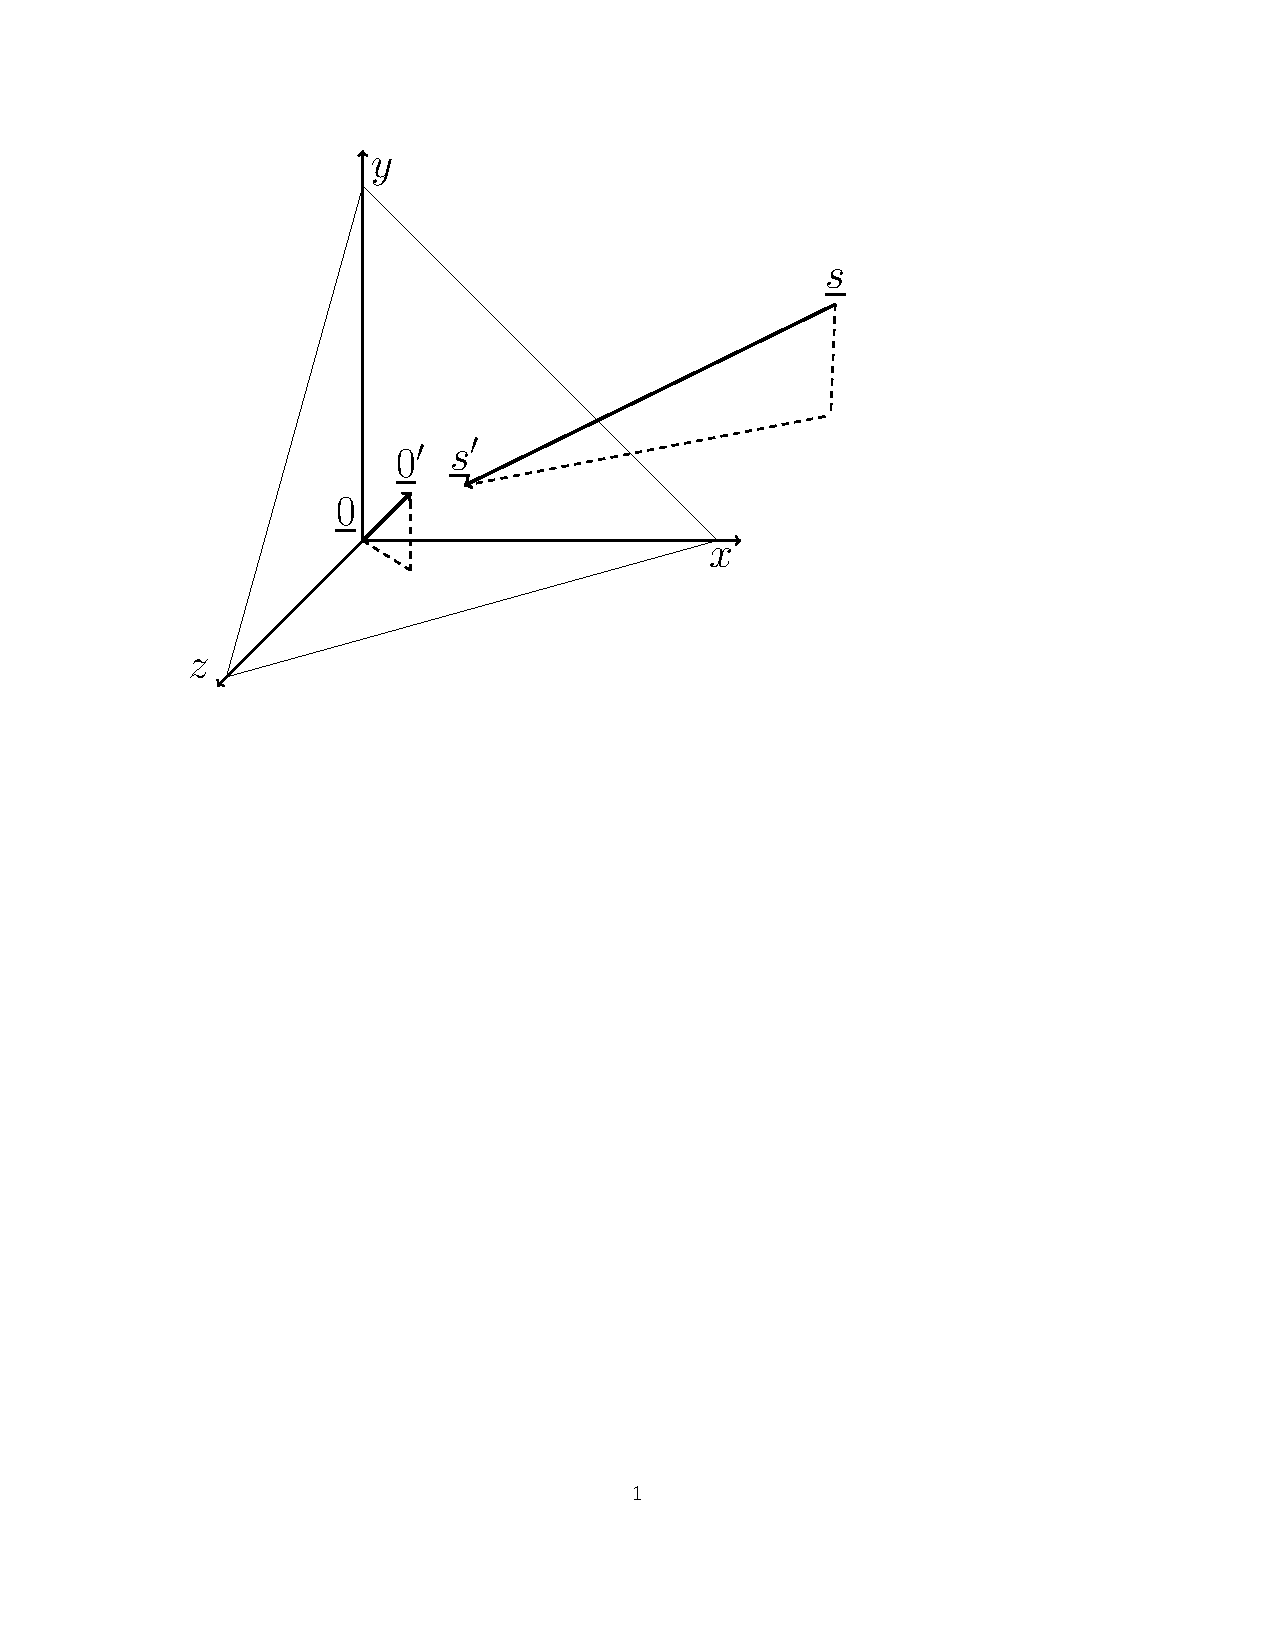
\includegraphics[trim={3cm 16cm 5cm 1cm},clip,scale=0.5]{figures/prob_plot_tikz_bw.pdf}}
%    & \num\putindeepbox[2pt]{\includegraphics[scale=0.25]{figures/real_space_tikz.png}} 
    & \subfigure[]{\includegraphics[trim={2cm 11cm 8cm 10.1cm},clip,scale=0.7]{figures/simple_tree_tikz.pdf}} \\
\end{tabular}
  \caption{In (a) we plot the points in the Euclidean space and the primed points represent the points mapped to the probability simplex, represented in the plot by the surface of the triangular plane given by the equation $x+y+z=1, x,y,z >0$. The primes indicate points on the probability simplex after applying the additive logistic transformation to the split counts. In (b) we plot an example decision tree splitting on two of three possible covariates.}
  \label{fig:trees_and_probability}
\end{figure}
 
 Consider Figure \ref{fig:trees_and_probability}; in this figure we have a plot of a decision tree and a plot of the probabilities associated with the tree on a two-dimensional simplex and the three-dimensional Euclidean space. If the observed data has only three covariates and we only observe the first two covariates, $x_1$ and $x_2$ in the estimated tree, then the covariate selection probability vector is approximately $\vec{p} = [0.50, 0.31, 0.19]$. The covariate that has no observed splits receives a lower assigned probability for the subsequent iteration, whereas the two covariates with larger numbers of splits receive proportionally higher covariate selection probabilities for the following iteration of the algorithm. Note the point $\vec{0}^\prime$ in Figure \ref{fig:trees_and_probability} is the point $(1/3,1/3,1/3)$ which functions as the origin on the simplex in 3 dimensions. 

This paper proceeds as follows: Section \ref{sec:Model} contains a description of the models used in this paper. Also in Section \ref{sec:Model}, we state the likelihood function and review the Chipman et al. Bayesian CART \cite{chipman1998bayesian} model for completeness.  In Section \ref{sec:ALoVaS_model}, we present the ALoVaS model, we show the relation with the CGM model, and detail the simulation algorithms used. Then in Section \ref{sec:Examples}, we present simulated examples where we study the efficacy of our proposed method using the regularization priors we describe in Section \ref{sec:Model}. Concluding Section \ref{sec:Examples}, we give an example classifying webpages according to whether those webpages contain ads or not. Finally, in Section \ref{sec:Conclusion} we summarize our findings and discuss the limitations, extensions, and possible variations of our work.      

\subsection{The Model}\label{sec:ALoVaS_model}

In this section we detail the ALoVaS model in the most general form. Then we detail the model for an arbitrary choice of priors for the means and variances. This allows the reader to see concrete examples of the ALoVaS method for clarity while preserving the general applicability of the method. 

We begin the model description by stating our posterior, 
\begin{equation}\label{eqn:post}
\pi(\mathcal{T}, \theta, \vec{q} \vert Y,X) \propto \mathcal{L}(Y \vert X, \mathcal{T}, \theta, \vec{q})\pi(\theta \vert \mathcal{T})\pi(\vec{q}\vert \mathcal{T})\pi(\mathcal{T}), 
\end{equation}
where $Y$ denotes the response vector, $X$ is the design matrix or the collection of covariates, $\mathcal{T}$ denotes the decision tree, and $\vec{q}$ denotes the vector of covariate selection probabilities. 

Instead of defining $\pi(\vec{q} \vert \mathcal{T})$ in terms of $\vec{q}$ we define on a linear scale, and once we have the linear scale parameters we convert to a probability using the \ALT
\begin{equation}\label{eqn:alt}
\vec{q} = \left[ q_1, q_2,\dots, q_{p-1}, q_p \right] =\vec{g}^{-1}(\vec{\mu})= \left[ \frac{e^{\mu_1}}{1+S_{p-1}},\frac{e^{\mu_2}}{1+S_{p-1}}, \dots,\frac{e^{\mu_{p-1}}}{1+S_{p-1}},\frac{1}{1+S_{p-1}} \right],
\end{equation} 
where the notation is the same as in Section \ref{sec:Introduction}. The parameters on the linear scale are denoted $\mu_j$ and can be interpreted as log-odds of selecting covariate $j$. The number of splits on each covariate at each iteration are denoted as $s_{jt}$. We assume these to have an approximately normal distribution once multiplied by a parameter $c_j$. The parameter $c_j$ is distributed on the support $[-1,1]$ and has a scaled-beta prior scaled and shifted to cover the support of $c_j$. This framework is written succinctly in Equations \ref{eqn:alovas1} and \ref{eqn:alovas2}. These equations are written out here for completeness

\begin{equation}\label{eqn:alovas1}
c_js_{jt} \vert c_j \sim N\left(\mu_j=log(q_j/q_p),\sigma_j^2\right),
\end{equation}

\begin{equation}\label{eqn:alovas2}
c_j \sim \text{ ScaledBeta}(-1,1,\alpha, \beta), \text{   and}	
\end{equation}

\begin{equation}\label{eqn:flavor_prior}
\mu_j \sim g(\mu_j). 
\end{equation}

Here the density function $g$ can be specified by the analyst. In this paper we detail the specification of $g$ as a double exponential (Equation \ref{eqn:lasso}) prior, SSVS (Equation \ref{eqn:ssvs}) prior, and horseshoe (Equation \ref{eqn:horseshoe}) prior. The form of $g$ should now be recognized as a regularization prior. In Appendix \ref{sec:appendix} we include details for each of the three stated priors. Namely, the pseudocode for the lasso, SSVS, and horseshoe priors may be found in Sections \ref{sec:lasso_app}, \ref{sec:ssvs_app}, and \ref{sec:horseshoe_app}, respectively.
Finally, we assume the usual Jeffreys' prior for the variances, 
\begin{equation}
\pi(\sigma^2_j) \propto \ \  \sigma^{-2}_j. 
\end{equation}

In practice inference should not be conducted on all the parameters in the model. There are many additional parameters in this model compared to the CGM version. For us, the main parameters of interest are $\mathcal{T}_i$, the $i$th decision tree and $\vec{q}$, the covariate selection probabilities. The probabilities are a function of the parameters $\vec{\mu},\vec{c},\vec{\sigma}$ and any other hyper-parameters estimated or sampled over. For full implementation details of the ALoVaS methods we study we include pseudocode in Appendix \ref{sec:appendix} for the SSVS, lasso, and horseshoe methods we implement. However, as noted in this section, different choices of $g(\mu_j)$ priors that regularize will result in different types of ALoVaS methods so the careful reader should be able to tailor the existing methods to whatever specific regularization prior they desire. 

 %We now describe the detailed balance criteria and give the equation that must be satisfied for this criteria to hold in our model. 
 The proposed trees are accepted or rejected based on the usual Metropolis-Hastings rule which is written here for completeness
 
 \begin{equation}
\alpha(\mathcal{T}\vert \mathcal{T}^\prime) = \text{min}\left(\frac{\Pr(\mathcal{T}^\prime \vert X, \vec{q}, \vec{y} )\Pr(\mathcal{T}| \mathcal{T}^\prime) }{ \Pr(\mathcal{T} \vert X, \vec{q}, \vec{y})\Pr(\mathcal{T}^\prime \vert \mathcal{T}) } ,1\right)
 \end{equation}
 
Detailed balance is a formal property imposed on Markov Chains after convergence. Intuitively, the detailed balance equation indicates that after convergence the process has the same distribution when run forwards in time as when run backwards in time. Formally, this is represented in Equation \ref{eqn:detailed_balance}, 
\begin{equation}\label{eqn:detailed_balance}
\alpha (\mathcal{T}^{(t)} \vert \mathcal{T}^{(t-1)}, \vec{q}^{(t-1)})\pi(\mathcal{T}^{(t)}\vert \vec{q}^{(t-1)})\pi(\vec{q}^{(t-1)}) = \pi(\vec{q}^{(t)}\vert \mathcal{T}^{(t-1)})\pi(\mathcal{T}^{(t-1)})\alpha(\mathcal{T}^{(t-1)} \vert \mathcal{T}^{(t-1)}, \vec{q}^{(t)} ),
\end{equation}
where the superscripts denote the (discrete time) nature of the Markov Chain. Where we are holding the $\vec{q}$ constant while transitioning from $\mathcal{T}^{(t)}$ to $\mathcal{T}^{(t-1)}$. Once the transition on $\mathcal{T}$ has been made we update $\vec{q}$ using a Gibbs step. Thus, our algorithm is a Metropolics within Gibbs algorithm. The Metropolis step updates $\mathcal{T}$ and the Gibbs step updates $\vec{q}$ and we iterate until convergence. It can be shown that any algorithm satisfying the detailed balance criteria is guaranteed to converge to the stationary distribution \cite{robert1999monte}. 

The Markov Transition Density (MTD),  for $q_j$ is given by Equation \ref{eqn:markov_trans_density}
\begin{equation}\label{eqn:markov_trans_density}
\Pr(q_j^{(t)}\vert q_j^{(t-1)})=\sum_{\mathcal{T}}\Pr(q_j^{(t)}\vert \mathcal{T}^{(t-1)})\Pr(\mathcal{T}^{(t-1)} \vert q_j^{(t-1)}).
\end{equation}
A similar MTD can be formulated for $\mathcal{T}$. When closed forms exist for these MTDs, and minorization and drift conditions are also satisfied, geometric convergence may be established. For examples and more details on this line of study, see the very readable introduction by Jones and Hobert \cite{jones2001honest}. For our example, the MTD for $\vec{q}$ involves evaluating an NP-Hard sum, thus exact convergence rates seem unlikely to be found. 

In this section we write out the ALoVaS model for a specific regularization prior. In general, the prior on the set $\{\mu_j,\sigma^2_j\}_{j=1}^{p}$ will change, giving us different flavors of the ALoVaS method. In this paper we include a study of the lasso, horseshoe, and SSVS priors, but other variations are certainly possible. Moreover, we do not claim optimality of our results. Indeed, many of these priors are optimal only in specific circumstances. If a model is not optimal in a linear model, this will carry over to our ALoVaS model and therefore, the ALoVaS method will be sub-optimal as well. This is not a drawback of our proposed ALoVaS method but is a drawback of the choice of the regularization prior in the given situation.  


\newpage
\chapter{ALoVaS Examples and a Case Study}\label{sec:Examples}

In this chapter we present simulation studies to illustrate properties of our methods. The two illustrated properties are handling multi-modality and handling highly non-balanced categorical response variable class probabilities. Following these simulation studies we present a case study using the internet ads dataset from the UC-Irvine machine learning database \cite{Frank:2010uq}. 

We first present simulated examples where we study the efficacy of our proposed method. We use the regularization priors we describe in Chapter \ref{sec:Introduction}. Concluding Section \ref{sec:real_data}, we give an example classifying webpages according to whether those webpages contain ads or not. Finally, in Section \ref{sec:Conclusion}, we summarize our findings and discuss the limitations, extensions, and possible variations of the ALoVaS model.     

	\section{Simulated Examples}
	In this section we present two collections of simulations. The first collection aims to study the effects of having multiple best trees in the generative model. The second collection aims to study the effects of class imbalance when dealing with a categorical response. 
	
%\subsubsection{Correlated Covariate Simulations}
%		
%		\begin{figure}[H]
%  \centering
%  \includegraphics[width=4in]{figures/scaled_shifted_beta_plots_bw.pdf}
%  \caption{Plots of the scaled-beta densities for the parameter settings we use to simulate correlation parameters. }
%  \label{fig:scaled_shifted_beta}
%\end{figure}
%
%We simulate data according to the linear regression model given by Equation \ref{def:linear_model}. The $X$ matrix contains row vectors of covariates denoted $\vec{x}_i^T$. The covariates are draws from a correlated multivariate normal density with the correlation matrix given by $4\nu I + \rho J$, where $I$ and $J$ are conformable identity and and all 1 matrices respectively. The parameter $\nu$ is sampled from an inverse gamma distribution with shape and scale parameters of $1/2$ and $1$. The parameter $\rho$ is sampled from one of the beta distributions given in Figure \ref{fig:scaled_shifted_beta} depending on which correlation scenario is given. Moreover, we simulate the random coefficients, $\vec{\mu}$, according to a continuous uniform distribution on the support $[-20,20]$. Thus, our simulations have scenarios of highly and weakly correlated covariates, as well as both positive and negative coefficients.
%
%%%% table of simulation results for correlated covariates simulations. 
%
%\begin{table}[H]
%\begin{center}
%\begin{tabular}{cc|c|c|c|c|c|c|}
%\cline{3-8}
%& & \multicolumn{6}{|c|}{Correlation Scenarios }\\  \cline{3-5}
%& & All High & All Mid & All Low  \\\cline{1-5}
%\multicolumn{1}{ |c| }{\multirow{3}{*}{50\% Sparsity} }  &
%\multicolumn{1}{ |c| }{SSVS} & 719679.05 &605340.89  &259739.80    \\  \cline{2-5}
%\multicolumn{1}{ |c| }{}&LASSO&321976.86  & 289537.96& 185282.31    \\ \cline{2-5}
%\multicolumn{1}{ |c| }{}&HORSESHOE  & 653732.97 &153722.46  &  445669.36 \\ \cline{1-5} 
%\multicolumn{1}{ |c| }{\multirow{3}{*}{60\% Sparsity} }  &
%\multicolumn{1}{ |c| }{SSVS} &591305.83  &507564.78  & 140295.82   \\  \cline{2-5}
%\multicolumn{1}{ |c| }{}&LASSO& 681873.23 &803175.40  &112567.28    \\ \cline{2-5}
%\multicolumn{1}{ |c| }{}&HORSESHOE  & 317808.78 & 205273.51 &199787.11   \\ \cline{1-5} 
%\multicolumn{1}{ |c| }{\multirow{3}{*}{70\% Sparsity} }  &
%\multicolumn{1}{ |c| }{SSVS} &42107.02  &36544.59  & 72987.87   \\  \cline{2-5}
%\multicolumn{1}{ |c| }{}&LASSO& 54788.10 & 26672.33 &  57799.72    \\ \cline{2-5}
%\multicolumn{1}{ |c| }{}&HORSESHOE  &62239.98& 33495.43 & 65066.95  \\ \cline{1-5} 
%\multicolumn{1}{ |c| }{\multirow{3}{*}{80\% Sparsity} }  &
%\multicolumn{1}{ |c| }{SSVS} &25452.16&28720.73 &4039.34 \\  \cline{2-5}
%\multicolumn{1}{ |c| }{}&LASSO&21379.87  &21292.66  &  3174.12     \\ \cline{2-5}
%\multicolumn{1}{ |c| }{}&HORSESHOE  & 34541.69 & 44203.84 & 2266.33  \\ \cline{1-5} 
%\multicolumn{1}{ |c| }{\multirow{3}{*}{90\% Sparsity} }  &
%\multicolumn{1}{ |c| }{SSVS} &18639.01 & 2299.55 &1302.07    \\  \cline{2-5}
%\multicolumn{1}{ |c| }{}&LASSO&20570.07  & 2877.12 &1467.92\\ \cline{2-5}
%\multicolumn{1}{ |c| }{}&HORSESHOE  & 27485.12 &1278.87  & 3230.96  \\ \cline{1-5} 
%\multicolumn{1}{ |c| }{\multirow{3}{*}{95\% Sparsity} }  &
%\multicolumn{1}{ |c| }{SSVS} &89319.59 &1309.86 &4894.39      \\  \cline{2-5}
%\multicolumn{1}{ |c| }{}&LASSO& 79849.77 & 1507.78 & 1124.96      \\ \cline{2-5}
%\multicolumn{1}{ |c| }{}&HORSESHOE  &21061.88 & 4186.80 & 1260.12  \\ \cline{1-5} 
%\multicolumn{1}{ |c| }{\multirow{3}{*}{99\% Sparsity} }  &
%\multicolumn{1}{ |c| }{SSVS} &12031.52  &2383.80  &1233.37    \\  \cline{2-5}
%\multicolumn{1}{ |c| }{}&LASSO&19271.86  &1287.68 & 1231.78     \\ \cline{2-5}
%\multicolumn{1}{ |c| }{}&HORSESHOE  &16897.56  &1726.18  & 3282.69 \\ \cline{1-5} 
%\end{tabular}
%\caption{Correlated simulation study results, each entry represents the MSE for that scenario and model. The MSE is calculated as $\sum_{i}(\hat{y}_{i}-y_i)^{2}/10000$, where $i$ runs from draw $1,000$ to $11,000$. Thus our burn-in is $1,000$.}
%\label{tab:corr_study_results}
%\end{center}
%\end{table}
%%%% end of table of simulation results for the correlated covariates simulations
%
%What is apparent from Table \ref{tab:corr_study_results} is that there is no clearly better flavor of ALoVaS. The choice of which method works best is likely to depend on the correlations of the covariates and the degree of sparsity present in the underlying data generating process. Moreover, We notice an increase in the mean squared prediction error as the sparsity decreases, in particular we notice a large increase as we move from a 90\% sparse data generating process to one that is less sparse. This corresponds with findings from Monte Carlo simulations the authors have conducted on the linear model equivalents of the three ALoVaS models. The finding that the best choice of method depends on unknown and difficult to estimate parameters is troubling from a practical standpoint. While it may be taken as a given that in genomics problems the sparsity of the underlying model is 99+\%, in many other application areas like insurance, econometric, and environmental statistics to name a few, the degree of sparsity is not so clear and may vary from less than 10\% to over 99\% depending on the data and the phenomenon being modeled.  

\subsection{Multimodal Simulation Study}
In this collection of simulations we study is a class of simulations where more than one model explains the data equally well. We simulate data according to the model described in Wu, Tjelmland, and West \cite{wu2007bayesian}, which exhibits multi-modality, also called the Rashomon effect by Breiman \cite{breiman2001statistical}. To simulate effectively from the data generating process, we need to be able to sample the two models in the same chain. 

For this simulated example we take $x_{i1} \sim \text{Unif}(.1,.4)$, for $i=1,\dots ,200$, and $x_{i1} \sim \text{Unif}(.6,.9)$, for $i=201,\dots,300$. Similarly, $x_{i2} \sim \text{Unif}(.1,.4)$, for $i=1,\dots ,100$, $x_{i2} \sim \text{Unif}(.6,.9)$, for $i=101, \dots,200$ , and $x_{i2} \sim \text{Unif}(.1,.9)$, for $i=201, \dots,300$. Finally, $x_{i3} \sim \text{Unif}(.6,.9)$ for $i =1, \dots 200$, and $x_{i3} \sim \text{Unif}(.1,.4)$, for $i=201, \dots,300$. Then, given these values, 

\[
 y_i =
  \begin{cases} 
      \hfill 1+N(0,0.25)    \hfill & \text{ if $x_{1i} \leq 0.5$ and $x_{2i} \leq 0.5$, } \\
      \hfill 3+ N(0,0.25) \hfill & \text{ if $x_{1i} \leq 0.5$ and $x_{2i} > 0.5$, } \\
      \hfill 5+ N(0,0.25) \hfill & \text{if $x_{1i} > 0.5$. }\\
  \end{cases}
\]

We run our algorithm using the regularized methods on the number of splits and then transform all the sampled $\mu_j$ using the \ALT. In this simulation, varying the sparsity is not something easily parametrized. Whereas in the next simulation we can vary the number of active covariates, in this simulation we must fix the number of active covariates to $3$ and vary the total number of covariates to accomplish a varying of the percentage of sparsity. Similarly to the next simulation, we compare the linear model methods: lasso, horseshoe, and SSVS. so for a sparsity of 50\% we simulate $x_1, \dots, x_6$ with the last three covariates being independent draws from standard normals higher sparsity percentages correspond to a larger number of additional standard normal covariates being independently sampled. The various models correspond to the rows within a sparsity level in Table \ref{tab:rashomon_study_results}.  

\begin{table}[H]
\begin{center}
\begin{tabular}{cc|c|c|c|}
  \\ \cline{3-3}
& & MSE  \\\cline{1-3}
\multicolumn{1}{ |c| }{\multirow{3}{*}{sparsity 50\%} } & 
\multicolumn{1}{ |c| }{CGM} & $34.74 \pm 12.27$\%  \\  \cline{2-3}
\multicolumn{1}{ |c| }{}&SSVS &$12.43 \pm 6.21$\%  \\  \cline{2-3}
\multicolumn{1}{ |c| }{}&LASSO& $5.89 \pm 3.48$\%    \\ \cline{2-3}
\multicolumn{1}{ |c| }{}&HORSESHOE &$7.35 \pm 8.21$ \%  \\ \cline{1-3}
\multicolumn{1}{ |c| }{\multirow{3}{*}{sparsity 60\%} } & 
\multicolumn{1}{ |c| }{CGM} &$34.44 \pm 9.62$ \%  \\  \cline{2-3}
\multicolumn{1}{ |c| }{}&SSVS & $9.64 \pm 5.81$\%    \\  \cline{2-3}
\multicolumn{1}{ |c| }{}&LASSO&$6.19 \pm 2.61$\%     \\ \cline{2-3}
\multicolumn{1}{ |c| }{}&HORSESHOE &$9.22 \pm 7.14$\%  \\ \cline{1-3}
\multicolumn{1}{ |c| }{\multirow{3}{*}{sparsity70\%} } & 
\multicolumn{1}{ |c| }{CGM} &$27.13 \pm 11.83$\%  \\  \cline{2-3}
\multicolumn{1}{ |c| }{}&SSVS &$8.41 \pm 5.79$\%    \\  \cline{2-3}
\multicolumn{1}{ |c| }{}&LASSO&$6.64 \pm 2.63$\%    \\ \cline{2-3}
\multicolumn{1}{ |c| }{}&HORSESHOE &$16.05 \pm 7.23$\%   \\ \cline{1-3}
\multicolumn{1}{ |c| }{\multirow{3}{*}{sparsity 80\%} } & 
\multicolumn{1}{ |c| }{CGM} & $27.64 \pm12.91$\%  \\  \cline{2-3}
\multicolumn{1}{ |c| }{}&SSVS &$8.69 \pm 3.43$ \%   \\  \cline{2-3}
\multicolumn{1}{ |c| }{}&LASSO&$6.12 \pm 1.01$\%    \\ \cline{2-3}
\multicolumn{1}{ |c| }{}&HORSESHOE &$7.52 \pm 5.21$\%  \\ \cline{1-3}
\end{tabular}
\caption{Multimodal simulation study results. Each entry represents the mean squared error of the optimal tree from the Markov chain. The numbers after the $\pm$ are the standard errors across the ten optima for the parallel chains. The $^*$ indicates that 3 cannot be divided by a number to get 60\% sparsity exactly. }
\label{tab:rashomon_study_results}
\end{center}
\end{table}

\begin{table}[H]
\begin{center}
\begin{tabular}{cc|c|c|c|}
  \\ \cline{3-3}
& & MSE  \\\cline{1-3}
\multicolumn{1}{ |c| }{\multirow{3}{*}{sparsity 90\%} } & 
\multicolumn{1}{ |c| }{CGM} &$68.06 \pm 13.76$ \%  \\  \cline{2-3}
\multicolumn{1}{ |c| }{}&SSVS &$11.94 \pm 4.68$ \%   \\  \cline{2-3}
\multicolumn{1}{ |c| }{}&LASSO& $8.41\pm 2.09$\%     \\ \cline{2-3}
\multicolumn{1}{ |c| }{}&HORSESHOE & $ 9.63\pm 7.89$\%   \\ \cline{1-3}
\multicolumn{1}{ |c| }{\multirow{3}{*}{sparsity 95\%} } & 
\multicolumn{1}{ |c| }{CGM} &$47.37 \pm 17.89$\%  \\  \cline{2-3}
\multicolumn{1}{ |c| }{}&SSVS & $7.08 \pm 4.37$\%    \\  \cline{2-3}
\multicolumn{1}{ |c| }{}&LASSO& $11.15\pm 3.70$\%     \\ \cline{2-3}
\multicolumn{1}{ |c| }{}&HORSESHOE &$8.98 \pm 3.88$ \%   \\ \cline{1-3}
\multicolumn{1}{ |c| }{\multirow{3}{*}{sparsity 99\%} } & 
\multicolumn{1}{ |c| }{CGM} & $47.51 \pm 18.31$ \%  \\  \cline{2-3}
\multicolumn{1}{ |c| }{}&SSVS & $6.82 \pm 3.17$\%   \\  \cline{2-3}
\multicolumn{1}{ |c| }{}&LASSO&$7.33 \pm 3.21$\%     \\ \cline{2-3}
\multicolumn{1}{ |c| }{}&HORSESHOE &$5.73 \pm  4.01$\%   \\ \cline{1-3}
\end{tabular}
\caption{Second table of multimodal simulation study results. Each entry represents the mean squared error of the optimal tree from the Markov chain. }
\label{tab:rashomon_study_results2}
\end{center}
\end{table}


 \begin{figure}[H]
  \begin{center}
\begin{tikzpicture}
 \node [circle,draw]{$X_1 \leq 0.5$} [level distance=25mm,sibling distance=50mm]
child { node [circle,draw]{$X_2 \leq 0.5$} [level distance=25mm ,sibling distance=25mm]
child {node [circle,draw] {}}
child {node [circle,draw]{}}
}
child {node [circle,draw] {} [level distance=25mm ,sibling distance=25mm]
};
\end{tikzpicture}
\hspace{1cm}
\begin{tikzpicture}
 \node [circle,draw]{$X_3 \leq 0.5$} [level distance=25mm,sibling distance=50mm]
child { node [circle,draw]{} [level distance=25mm ,sibling distance=25mm]
}
child {node [circle,draw] {$X_2 \leq 0.5$} [level distance=25mm ,sibling distance=25mm]
child {node [circle,draw] {}}
child {node [circle,draw]{}}
};
\end{tikzpicture}
\caption{The two optimal trees for the multimodal simulation study. }
\label{fig:best_two_trees}  
\end{center}
\end{figure}
For the results presented in Table \ref{tab:rashomon_study_results} our burn-in is $1,000$. Additionally, we calculate MSEs using the 10,000 observations after burn in. Convergence diagnostics indicated a minimum sample size of 3746, so 10,000 samples is beyond adequate. 
 
Moreover, in Table \ref{tab:rashomon_study_results} a sentiment appears. There is no clear winner across sparsity levels. While the lasso and the horseshoe appear to be competitive at higher sparsity levels, the SSVS method might also be competitive at lower and higher sparsity levels but there is some degree of variability across the sparsity levels. Additionally, while all three models are able to attain one of the two modes, all three models have difficulty moving from one of the two modes in the underlying model to the other mode. This is exactly a result of the sparsity imposed on the fitted model. The two posterior trees in the two modes have different sets of covariates and thus the sparsity patterns will have difficulty switching from one to the other. A similar pattern can be found in sparse linear models. Typically, correlation constraints are imposed on the $(X^TX)$ matrix to ensure consistency of the selected sparsity pattern. 

\subsection{Class Unbalancedness Simulation Study}
We next perform a simulation on unbalanced response class probabilities. We examine various states of unbalancedness of the categorical response variable. The intent of this simulation study is to determine the effect of response class unbalancedness, a phenomenon widely seen in statistical practice. We simulate data according to the $3$ category logistic regression model with a varying number of covariates. In this simulation we fix the number of active covariates to $2$ so that varying the sparsity requires the number of covariates to range from $4$ total (sparsity =$50\%$) to $200$ total ($99\%$ sparsity). For convenience we fix the coefficient vector at $\vec{\beta}^T =[1,1,0,\dots, 0]$, varying the dimensionality of the $\beta$ vector as necessary for the desired sparsity. We vary the means of the normal distributions of the first two covariates to achieve the desired class response probabilities for the three classes. The additional covariates, added as noise, and to increase the sparsity are simulated as independent standard normal draws drawn independently of each other and across observations. We include Figure \ref{fig:simulated_unbalanced_simplex} to give the reader a visual idea of the points on the three dimensional simplex where we study the class unbalanced problem. Note that by the self-similarity of the simplex space we don't need to study the areas of the simplex that are empty. Switching the labeling of the axes accomplishes this for us. In this case the settings where certain classes are extremely rare require a sample of $n=10000$ per simulation. This setting is used for the highly unbalanced cases, as well as all the other cases in Figure \ref{fig:unbalanced_study_results}.

\begin{figure}[H]
\begin{center}
\begin{tikzpicture}
	[scale=4,
		axis/.style={->,black,thick},
		vector/.style={-stealth,black,very thick},
		vector guide/.style={dashed,black,thick}]
	\coordinate (O) at (0,0,0);
	\draw[axis] (0,0,0) -- (1.6,0,0) node[anchor=north east]{$x$};
	\draw[axis] (0,0,0) -- (0,1.6,0) node[anchor=north west]{$y$};
	\draw[axis] (0,0,0) -- (0,0,1.6) node[anchor=south]{$z$};
	\coordinate (A) at (1.1,0,0);
\coordinate (B) at (0,1.1,0);
\coordinate (C) at (0,0,1.1);
\coordinate[label=above left:$\underline{0}$] (D) at (0,0,0);
\coordinate[label=above:$ \bullet$] (D') at (0.333,0.333,0.333);
\coordinate[label=above:$ \bullet$] (D'') at (0.5,0.25,0.25);
\coordinate[label=above:$ \bullet$] (D''') at (0.6,0.2,0.2);
\coordinate[label=above:$ \bullet$] (D') at (0.8,0.1,0.1);
\coordinate[label=above:$ \bullet$] (D') at (0.98,0.01,0.01);
\coordinate[label=above:$ \bullet$] (D') at (0.998,0.001,0.001);
%\coordinate[label=above:$ \bullet$] (E) at (0.45,0.45,0.1);
%\coordinate[label=above:$ \bullet$] (F) at (0.4,0.4,0.2);
%\coordinate[label=above:$ \bullet$] (G) at (0.7,0.25,0.05);
%\coordinate[label=above:$ \bullet$] (H) at (0.85,0.1,0.05);
%\coordinate[label=above:$ \bullet$] (H) at (0.55,0.3,0.05);
\coordinate (Oxz) at (0.33,0,0.33);
\coordinate (Pxy) at (2, 0.55, 0.05);
\coordinate (R) at (0.165,0.66,0.165);
\coordinate (R') at (1.4,1.08,0);
\draw (A)--(B)--(C)--cycle;
\path (A) -- (B) -- (C) -- cycle;
\end{tikzpicture}
\caption{The points on the three dimensional simplex space we use as unbalanced classes in the simulation study. }
\label{fig:simulated_unbalanced_simplex}
\end{center}
\end{figure}

%class_imbalance_50_sparsity.pdf

\begin{figure}[H]
\begin{center} 
\begin{tabular}{cc}
 \subfigure[]{\includegraphics[scale=0.4]{figures/class_imbalance_50_sparsity1.pdf}}
    & \subfigure[]{\includegraphics[scale=0.4]{figures/class_imbalance_60_sparsity1.pdf}} \\
  \subfigure[]{\includegraphics[scale=0.4]{figures/class_imbalance_70_sparsity1.pdf}}
    & \subfigure[]{\includegraphics[scale=0.4]{figures/class_imbalance_80_sparsity1.pdf}} \\
   \end{tabular}
\caption{ Box plots of the errors in prediction with the hold out data from the sampled trees after burn-in in the unbalanced simulation study. The three box plots are the prediction errors for the sampled trees for SSVS, lasso, and horseshoe within each set of class probabilities. The fractions displayed with each set of four box plots label the  correspondence with the proportion used to simulate each of the three response classes in the simulated data. Also these proportions are the points on the simplex displayed in Figure \ref{fig:simulated_unbalanced_simplex}. Each letter in the figure, corresponding to the different box plots is a different sparsity value, corresponding to different sparsity levels in the number of covariates. Figure  (a) corresponds to 50\% sparsity, Figure (b) 60\%, Figure (c) 70\%, and Figure (d) 80\%. }
\label{fig:unbalanced_study_results}
\end{center}
\end{figure}

\begin{figure}[H]
\begin{center} 
   \subfigure[]{\includegraphics[scale=0.4]{figures/class_imbalance_90_sparsity1.pdf}}
     \subfigure[]{\includegraphics[scale=0.4]{figures/class_imbalance_95_sparsity1.pdf}} \\
\subfigure[]{\includegraphics[scale=0.4]{figures/class_imbalance_99_sparsity1.pdf}}
\caption{ Box plots of the errors in prediction with the hold out data from the sampled trees after burn-in in the unbalanced simulation study. This is for the case of 90\% (a) sparsity, 95\% (b) sparsity, and (c) 99\% sparsity. }
\label{fig:unbalanced_study_results2}
\end{center}
\end{figure}

%\begin{table}[H]
%\begin{center}
%\begin{tabular}{cc|c|c|c|c|c|c|}
%\cline{3-8}
%& & \multicolumn{6}{|c|}{Class Imbalance Scenarios }\\  \cline{3-8}
%& & \tiny{(1/3,1/3,1/3)} & \tiny{(1/4,1/4,2/4)} & \tiny{(1/5,1/5,3/5)}  & \tiny{(1/10,1/10,8/10)} &\tiny{(1/100,1/100,98/100)} & \tiny{(1/$10^3$,1/$10^3$,998/$10^3$)}\\\cline{1-8}
%\multicolumn{1}{ |c| }{\multirow{3}{*}{Sparsity 50\%} } & 
%\multicolumn{1}{ |c| }{SSVS} &0.00\%  &0.00\%  & 0.30\% &0.00\%  &0.00\%&0.80\%  \\  \cline{2-8}
%\multicolumn{1}{ |c| }{}&LASSO&0.00\%  &0.00\%  &0.00\%  &0.00\%   &0.00\%  &0.10\%     \\ \cline{2-8}
%\multicolumn{1}{ |c| }{}&HORSESHOE  &0.20\%  &0.10\%  &0.00\%  &0.00\%  &0.20\%  &0.10\%\\ \cline{1-8}
%\multicolumn{1}{ |c| }{\multirow{3}{*}{Sparsity 60\%} } & 
%\multicolumn{1}{ |c| }{SSVS} &0.39\%  &0.10\%  & 0.10\% &0.00\%  &0.20\%&0.40\%  \\  \cline{2-8}
%\multicolumn{1}{ |c| }{}&LASSO&0.27\%  &0.25\%  &0.00\%  &0.00\%   &0.00\%  &0.10\%     \\ \cline{2-8}
%\multicolumn{1}{ |c| }{}&HORSESHOE  &0.20\%  &0.09\%  &0.08\%  &0.00\%  &0.00\%  &0.50\%\\ \cline{1-8}
%\multicolumn{1}{ |c| }{\multirow{3}{*}{Sparsity 70\%} } & 
%\multicolumn{1}{ |c| }{SSVS} &0.13\%  &0.24\%  &0.30\%  &0.04\%  &0.00\%&0.60\%  \\  \cline{2-8}
%\multicolumn{1}{ |c| }{}&LASSO& 0.10\% &0.15\%  &0.20\%  &0.00\%   &0.00\%  &0.30\%     \\ \cline{2-8}
%\multicolumn{1}{ |c| }{}&HORSESHOE  &0.10\%&0.30\%  &0.00\%  &0.00\%  &0.00\%  &0.40\%\\ \cline{1-8}
%\multicolumn{1}{ |c| }{\multirow{3}{*}{Sparsity 80\%} } & 
%\multicolumn{1}{ |c| }{SSVS} &1.012\%  &1.05\%  &0.10\%  &0.40\%  &0.01\%&0.40\%  \\  \cline{2-8}
%\multicolumn{1}{ |c| }{}&LASSO&0.50\%  &0.50\%  &0.40\%  & 0.40\%  & 0.40\% &0.38\%     \\ \cline{2-8}
%\multicolumn{1}{ |c| }{}&HORSESHOE  &0.08\%  &0.20\%  &0.00\%  &0.38\%  &1.20\%  &0.40\%\\ \cline{1-8}
%\multicolumn{1}{ |c| }{\multirow{3}{*}{Sparsity 90\%} } & 
%\multicolumn{1}{ |c| }{SSVS} &2.77\%  &0.20\%  &1.50\%  &1.15\%  &1.01\%&0.20\%  \\  \cline{2-8}
%\multicolumn{1}{ |c| }{}&LASSO&1.97\%  &1.20\%  &1.70\%  &1.40\%   &0.95\%  & 1.30\%    \\ \cline{2-8}
%\multicolumn{1}{ |c| }{}&HORSESHOE  &1.16\%  &0.40\%  &1.84\%  &0.02\%  &0.36\%  &0.50\%\\ \cline{1-8}
%\multicolumn{1}{ |c| }{\multirow{3}{*}{Sparsity 95\%} } & 
%\multicolumn{1}{ |c| }{SSVS} & 0.53\% &0.40\%  &7.51\%  &3.27\%  &0.79\%&0.21\%  \\  \cline{2-8}
%\multicolumn{1}{ |c| }{}&LASSO&0.00\%  &1.20\%  &3.96\%  &2.26\%   & 1.22\% & 0.80\%    \\ \cline{2-8}
%\multicolumn{1}{ |c| }{}&HORSESHOE  &1.96\%  &6.29\%  &1.74\%  &8.08\%  &1.40\%  &0.50\%\\ \cline{1-8}
%\multicolumn{1}{ |c| }{\multirow{3}{*}{Sparsity 99\%} } & 
%\multicolumn{1}{ |c| }{SSVS} &16.52\%  &16.43\%  &14.28\%  &0.20\%  &2.39\%& 0.10\% \\  \cline{2-8}
%\multicolumn{1}{ |c| }{}&LASSO&14.40\%  &16.21\%  &7.36\%  &3.23\%   &1.62  &0.50\%     \\ \cline{2-8}
%\multicolumn{1}{ |c| }{}&HORSESHOE  &16.78\%  &3.36\%  &16.43\%  &7.78\% &0.70\%  &7.78\%\\ \cline{1-8}
%\end{tabular}
%\caption{Class unbalancedness simulation study results, each entry represents the MSE for that scenario and model. The MSE is calculated as $\sum_{i}(\hat{y}_{i}-y_i)^{2}$, where $i$ runs from draw $1,000$ to $10,000$. Thus our burn-in is $1,000$.}
%\label{tab:unbalanced_study_results}
%\end{center}
%\end{table}

Intuitively, the results of Figures \ref{fig:unbalanced_study_results} and \ref{fig:unbalanced_study_results2} make sense. The less sparse the true model, the easier the model can classify the categories. Sparse models are not terribly difficult to classify. However, cases of extreme sparsity, such as those where 99+\% sparsity exists, are likely to have a far greater error rate. Interestingly, the degree of imbalance in the true, underlying model appear to affect the error as well. The explanation here is that, a decision tree can more easily partition a subset of the covariate space to classify responses that are rare as compared to more prevalent responses.

The results here are somewhat inconclusive on which specific model, ssvs, lasso, or horseshoe is best in a given scenario. It appears from the unbalanced simulation studies that, aside from Monte Carlo variability, there is no clear winner amongst the three ALoVaS models. It does appear that given a certain sparsity and perhaps other characteristics of the underlying model, such as correlation or class unbalanceness, it may be better to choose one type of ALoVaS model over the others. However, this information seems unlikely to be known \emph{a priori} except in special circumstances. Moreover, any of the ALoVaS methods is likely to prove useful and provide improvements over the traditional Bayesian decision tree algorithm proposed by CGM. 

\section{Case Study}\label{sec:real_data}

In this section we compare the ALoVaS method against the CGM approach, a variable importance (VIMP) based frequentist method \cite{ishwaran2010high}, and a non-decision tree based approach, the logistic-lasso. We compare these methods using the publicly available internet ads dataset from the UCI data repository \cite{Frank:2010uq}. The internet ads data set contains 1558 covariates, some numeric and some categorical. The data set was first used in a paper by Kushmerick \cite{kushmerick1999learning} and has since been used in several statistical classification studies. A more complete description of the data and references to other papers using this dataset can be found at the UCI machine learning repository website, at the following link: \url{https://archive.ics.uci.edu/ml/datasets/Internet+Advertisements}.

As noted by Kushmerick \cite{kushmerick1999learning}, there are several reasons for wanting to remove advertisements from webpages. Some reasons are: images tend to dominate a pages total download time, users dislike paying for services indirectly through advertisers preferring direct payment for services rendered, and malicious software can be unintentionally placed on a user's machine through images masked as advertisements. 

		\begin{table}[H]
\begin{center}
\begin{tabular}{|c|c|} \hline
Model & Error \\ \hline
ALoVaS-SSVS&$7.48 \pm 2.01$\%\\ \hline
ALoVaS-Lasso &$5.12 \pm 1.38$\% \\ \hline
ALoVaS-Horseshoe& $5.40 \pm 3.22$\% \\ \hline
VIMP& $15.30 \pm 4.10$\%\\ \hline
CGM& $7.20 \pm 3.57$\%\\ \hline
Logistic-lasso&$11.20 \pm 4.11$\%\\ \hline
\end{tabular}
\caption{Class unbalancedness simulation study results, each entry represents the MSE for that scenario and model. }
\label{tab:ads_misclass}
\end{center}
\end{table}

	
\begin{figure}[H]
\begin{center} 
\begin{tabular}{cc}
 \subfigure[]{\includegraphics[scale=0.35]{figures/CGM.png}}
    & \subfigure[]{\includegraphics[scale=0.35]{figures/ads_dataset_lasso_tree.pdf}} \\
  \subfigure[]{\includegraphics[scale=0.35]{figures/ads_dataset_ssvs_tree.pdf}}
    & \subfigure[]{\includegraphics[scale=0.35]{figures/ads_dataset_horseshoe_tree.pdf}} \\
    \end{tabular}
\caption{The  decision trees fitted to the internet ads dataset. The CGM (a) is much deeper than the remaining three trees fit using the ALoVaS method. The SSVS (b), Lasso (c) and horseshoe (d) all select the 1245th variable along with a second variable. The second variable differs in each of the three ALoVaS variants we use but the fact that the 1245th variable is common to all three gives further credence to the claim that a choice between the SSVS, lasso, or horseshoe types of ALoVaS is largely a choice of personal preference. }
\label{fig:unbalanced_study_results_trees}
\end{center}
\end{figure}
	
	
%	\begin{figure}[H]
%  \centering
%  \includegraphics[width=4in]{figures/CGM.png}
%  \caption{The tree fit using the CGM approach.}
%  \label{fig:CGM_tree}
%\end{figure}	
%
%%	\begin{figure}[H]
%%  \centering
%%  \includegraphics[width=4in]{figures/ad_tree.pdf}
%%  \caption{The tree fit using the greedy approach.}
%%  \label{fig:greedy_tree}
%%\end{figure}	
%
%	\begin{figure}[H]
%\begin{center}
%  \includegraphics[scale=0.3]{figures/ads_dataset_lasso_tree.pdf}
%  \caption{The lasso ALoVaS decision tree. }
%  \label{fig:horseshoe_ads_tree}
%  \end{center}
% \end{figure}		
%
%	\begin{figure}[H]
%\begin{center}
%  \includegraphics[scale=0.3]{figures/ads_dataset_ssvs_tree.pdf}
%  \caption{The ssvs ALoVaS decision tree. }
%  \label{fig:ssvs_ads_tree}
%  \end{center}
% \end{figure}	
%
%	\begin{figure}[H]
%\begin{center}
%  \includegraphics[scale=0.3]{figures/ads_dataset_horseshoe_tree.pdf}
%  \caption{The horseshoe ALoVaS decision tree. }
%  \label{fig:horseshoe_ads_tree}
%  \end{center}
% \end{figure}		
%		
		We use a random subset of the internet ads data to fit a CGM tree and an ALoVaS tree. We first remove all observations that contain missing values. We then take a 50\% random sample of training and test data. The MSE is calculated as $\sum_{i}(\hat{y}_{i}-y_i)^{2}$/10,000, where $i$ runs from draw $1,000$ to $11,000$. Thus our burn-in is $1,000$. Figure \ref{fig:unbalanced_study_results_trees} shows the estimated trees. The misclassification probabilities are calculated by dropping all data points from the test data set through the trees built using the training data. The resulting trees are fit using only the training data.  In this example we do not know the ground truth, so comparison of misclassification rates against a ground truth is not possible. Nevertheless, we compare misclassification rates amongst the models shown in Table \ref{tab:ads_misclass}. 
		
		From the misclassification errors shown in Table \ref{tab:ads_misclass}, it is clear that some of the trees compete with each other in terms of prediction. However, once we examine the images of the fitted decision trees in Figure \ref{fig:unbalanced_study_results_trees} ,we see that there is a dramatic difference in terms of the complexity of the tree for a given prediction error. The ALoVaS models are able to select trees with maximum depth of 2 and achieve comparable error rates to the CGM tree which has more splits on more variables. 
		
		Comparing the different decision trees selected by the three types of ALoVaS methods indicates that there is little practical difference between the SSVS, lasso, and horseshoe ALoVaS methods. Additionally, the variables selected by the three ALoVaS methods are very similar. Hence, the ALoVaS method is relatively insensitive to the regularization method used. Saying that, it is clear that there is a substantive performance increase over non-sparse competitors such as the CGM method and the logistic lasso. CGM is a nonlinear dense method, whereas logistic lasso is a linear, sparse method. In a nutshell, ALoVaS merges the benefits of both CGM and the lasso. The variable 1245 indicates that the webpage includes in the url the term `psu.edu', showing that at the time the internet ads dataset was collected, Penn state's website was hosting advertisements. The other variable that is commonly occurring is variable 353, which indicates that the url term contains the text string `images+ads', which seems to be an obvious choice of predictor. Further the variable 1337 indicates that the url string contained the set of characters `sj', which is a difficult set of characters to interpret and is likely ancillary information. 
		
		The take home point of this section is that, not only is the ALoVaS method a useful conceptual method for performing variable selection when fitting Bayesian decision trees, but it is also practically useful. The ALoVaS method is capable of handling data with a large number of covariates and of performing covariate filtering by choosing various covariates. As a byproduct of the fitting method we also generate a sampled set of covariate selection probabilities which can be used if the method is to be compared with other methods that perform variable selection and use a similar approach. 

\section{Conclusions}\label{sec:Conclusion}

A lot of press is given to variable selection methods, both in terms of theoretical properties and in terms of practical results. However, these applications nearly always implement linear or generalized linear models. Non-linear models, such as decisions trees, are mathematically less tractable and thus theoretical results are more difficult to derive. Our ALoVaS method facilitates variable selection methods familiar to the researcher and allows their use with decision tree models. In non-sparse settings our method experiences similar difficulties as those experienced by methods such as the lasso and horseshoe. This is not a limitation of our method \emph{per se} but rather an effect of model misspecification. 

One difficulty with the ALoVaS method proposed in this article is that exact zeros and ones are impossible unless $\Pr(\mu_j \in \{-\infty,\infty\})\neq 0$. This is a difficulty of all models using the ALN density and was noted by Atchison and Shen \cite{atchison1980logistic}, as a point in need of remedy. Although exact zero covariate selection probabilities are not theoretically possible with our model, we are able to create sparse, simple decision trees via the ALN density by estimating zero probabilities as numerically negligible. 

Of course, there are other distributions defined on the simplex that one might find useful to use for variable selection with decision trees. Perhaps using one of the distributions on the simplex from J\o rgensen's \cite{jorgensen1997theory} dispersion model apparatus would be a fruitful line of research. However, analytical intractability would result from using this type of distribution. Additionally, one would need to generalize the definition of this density to a simplex on more than 2 dimensions. Perhaps, if other densities on the simplex are deemed applicable, the application of those densities to decision tree variable selection could follow a line of reasoning similar to that described here. 

%future work? 
There remain several avenues of future work based on the findings documented in this manuscript. We list three:

\begin{itemize}
\item Explore other regularization methods that have non-zero probability of setting $\mu_j=0$. 
\item Study the effect of imposing normality on the split counts, $s_{ij}$ instead of a Poisson or negative binomial model. 
\item Study the effects of multiplicity adjustments, false positives, and false negatives in the models detailed. 
\end{itemize}

Regarding the first comment, the model proposed by Bhattacharya, Pati, Pillai, and Dunson \cite{bhattacharya2012bayesian} might be a useful first step. For the second item listed, the Gibbs sampling method proposed by Polson, Scott, and Windle \cite{polson2013bayesian} seems to be the way forward. Finally, regarding the last item, the arguments in Scott and Berger \cite{scott2010bayes}, as well as Efron's many articles and book length treatise \cite{efron2009empirical,efron2004large,efron2007correlation,efron2010large}, are logical starting points. 

In this Chapter and the previous Chapter we proposed a novel framework for linking variable selection or regularization methods from linear models with variable selection in decision tree models. Moreover, we compared simulated and real data using our proposed ALoVaS method against common competitors, such as the logistic lasso and the CGM decision tree approach. Our ALoVas method showed improved prediction errors over the logistic lasso and the CGM methods. Moreover, our method provided sparser, less deep decision trees compared to other decision tree methods. This allows easier interpretation of the model both for trained analysts and for non-technical stakeholders. While it is inevitable that limitations exist with all methods, it appears that for sparse data generating processes where a simple structural model is desired, our ALoVaS method is to be preferred.  


\newpage
\chapter{Synthesis: Comparing the DiVaS and ALoVaS Methods}
In this chapter we compare the DiVaS and ALoVaS models. While both methods seem relatively similar, both methods performing variable selection for Bayesian decision trees, there are fundamental practical and theoretical differences between the two methods. 

\section{Theoretical differences and a simulation study}

One of the most apparent theoretical differences between the DiVaS and ALoVaS models is the way the two models handle the correlation between covariate selection probabilities. One of the properties of the Dirichlet distribution is that $Corr(p_i,p_j) < 0$ for $i\neq j$. Thus, if the prior puts zero probability on non-negative covariate selection probability correlations, then the posterior will also place zero probability on these non-negative correlations. Figure \ref{fig:corr_divas_alovas} plots the relationship of the DiVaS and ALoVaS methods in the correlation space of two arbitrary covariate selection probabilities $(p_i,p_j)$. This section elucidates the differences between the two methods and compares the similarities. 


%%%% Start of graphic

%\PreviewEnvironment{tikzpicture}
%\setlength\PreviewBorder{5pt}%
\begin{figure}[H]
\begin{center}
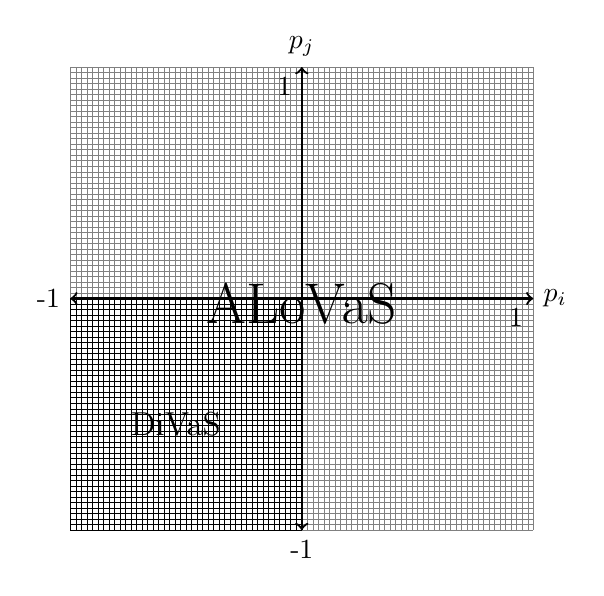
\begin{tikzpicture}[scale=.35]%\footnotesize
% grid
 
  %\draw[step=0.1cm,gray,very thin] (\xone,\yone) grid (8,8);
  \draw[step=0.2cm,gray,very thin] (-.4,-.4) grid (16.4,16.4);
  \draw[step=0.2cm,black,very thin] (-.4,-.4) grid (8,8);

% ticks
  \foreach \x/\xtext in { 8/\frac{1}{2}, 16/1}
  \draw[gray, very thin,xshift=\x cm] (0,.3) -- (0,-0.3) node[below] {};
  \draw[gray, very thin] (0,-0.3) node[below] {};
  \foreach \y/\ytext in {8/\frac{1}{2},16/1}
    \draw[gray, very thin, yshift=\y cm] (.3,0) -- (0,0)
    node[left] {};

% origin
 \draw[gray] (0,0) node[anchor=north east] {};

% labels 
\draw (3.43,3.43) node[circle]{\large{DiVaS}} circle (0cm);
\draw[thick] (8,7.8) node[]{\huge{ALoVaS}} circle (0cm);

% axes
  \draw[black,thick,<->] (-.4, 8) -- (16.4, 8) node[right] {$p_i$};
  \draw[black,thick,<->] (8, -.4) -- (8, 16.4) node[above] {$p_j$};
   \draw[black,thick] (16.4, 8) node[below left] {1};
  \draw[black,thick] (-.4, 8) node[left] {-1};
   \draw[black,thick] (8,16.4) node[below left] {1};
  \draw[black,thick] (8, -.4) node[below] {-1};

%  \draw[black,thick,<->] node[above] {$p_j$};
\end{tikzpicture}
\end{center}
\caption{A plot of the Correlation space where non-zero prior probability is placed in the DiVaS and ALoVaS models.}
\label{fig:corr_divas_alovas}
\end{figure}

%%%% End of graphic


One might be tempted to conclude that this is a element of minut\ae\ that has no practical consequence but consider a linear model data generating process that contains an interaction between two variables, $x_1$ and $x_2$

\begin{equation}\label{eqn:interaction_model}
y_i = \beta x_1x_2 + \epsilon_i,
\end{equation}  
where $\epsilon_i \sim N(0, \sigma^2$). In this case the coefficient $\beta$ controls the degree of curvature in the ($x_1, x_2$) space. The positive covariate selection probability results from using a constant function in each terminal node to approximate a curved two dimensional surface. The constant function requires alternating splits between $x_1$ and $x_2$ to approximate the curving of the ($x_1$, $x_2$) space. Thus, we see that there are really two important pieces to the model specification when fitting decision trees: specifying a tree model and specifying a terminal node model. Misspecification of one can lead to errors in the other, indicating that the two are also not independent.

A nice property of the ALoVaS method is that if $p_i$, $p_j$ are the two covariate selection probabilities, and if these $p_i$, $p_j$ have a logistic normal density, then the covariance between the two densities is 

\begin{equation}\label{eqn:cov_aln}
Cov(log(p_j / p_k), log(p_l / p_m) ) = \sigma_{jl} + \sigma_{km} - \sigma_{jm} - \sigma_{kl},
\end{equation}
where $\sigma_{ij}$ is the covariance parameter for the normal random variable before the application of the ALT. Clearly the four $\sigma_{ij} \geq 0$ in Equation \ref{eqn:cov_aln}, so that the covariance could be positive or negative.  

At this point it is worth noting that the idea of an automatic interaction detector was first proposed in the Chi-squared Automatic Interaction Detection (CHAID) \newabbrev{abbrev:CHAID} method \cite{kass1975significance}. The CHAID method claims to automatically detect interactions, yet popular documents \cite{ville2006decision} claim that CHAID and other decision tree methods cannot actually perform automatic interaction detection. The validity of this claim is not the point of this paragraph but it should be clear to the reader how one could visually inspect a fitted tree and determine if interaction is plausible. Moreover, if the ALoVaS method automatic interaction detection is plausible, by comparing the sampled values of $Cov(log(p_j/p_k), log(p_l/p_m) )$, or equivalently $Corr(p_i, p_j)$, with the point zero, one has an indication of the degree of interaction. Additionally, we cannot determine if the interaction is positive or negative, only that an interaction is present. If there was a desire to determine the sign of the interaction, then the analyst would need to provide estimates of the parameters in Equation \ref{eqn:cov_aln}. Alternately, we might estimate directly $Corr(p_i, p_j)$ with the Bayesian approach we take in the ALoVaS method. Either approach is feasible. 

We now present a small simulation study. We sampled data according to the model describing in Equation \ref{eqn:interaction_model}. We simulated $n=500$ observations from this model for a training dataset and another for a test, or hold-out dataset. We simulated data under the model with $\beta \in \{5, -5\}$. Figure \ref{fig:interaction_trees} plots the two trees fitted under a greedy optimization for the two interaction coefficients. 

\begin{figure}
\begin{center} 
\begin{tabular}{cc}
\includegraphics[scale=0.25]{figures/divas_tree_alovas_divas_compare.pdf}
\end{tabular}
\caption{The optimal DiVaS tree.}
\label{fig:interaction_trees}
\end{center}
\end{figure} 

We ran the ALoVaS and DiVaS algorithms for $11,000$ samples discarding the first $1000$ as a burn-in sample. Convergence statistics were calculated using the coda package in R with convergence statistics indicating a minimal sample size of 3764 and 3271 for the ALoVaS and DiVaS chains respectively. Figure \ref{fig:chain_max_interaction_tree} presents the trees with the largest integrated likelihood for the two chains.  

\begin{figure}
\begin{center} 
\begin{tabular}{cc}
\includegraphics[scale=0.25]{figures/lasso_compare_tree.pdf}
\end{tabular}
\caption{The optimal ALoVaS tree.}
\label{fig:chain_max_interaction_tree}
\end{center}
\end{figure} 

\section{Practical differences and a simulation study}

While the theoretical differences are important to academics and applied researchers who want to understand the limitations of a specific method, the questions most applied researchers tend to have are more practical in nature. We address the practical questions in this section. 

Practically speaking, the ALoVaS and the DiVaS methods are different in how you think about selecting a variable to split on, or to remove, from the current decision tree. While the DiVaS method allows us to \emph{quantify} these different scenarios, it does not allow us to think about these values in a manner we are familiar with. On the other hand, the ALoVaS method allows us a nice, linear framework to understand these differences. The primary difficulty lies in no standard, intuitive, basis to describe the simplex, the space of values in $d$ dimensions such that $\sum_jq_j=1$ and $q_j \geq 0$. Aitchison \cite{aitchison1986statistical} discussed several bases, none of which are intuitive, whereas Euclidean geometric space is intuitive, ubiquitous, and statisticians usually have experience with the Euclidean space.   

There are other more practical differences between the DiVaS and ALoVaS methods. For example, the ALoVaS method takes much longer to simulate. This increased simulation time should be no surprise given the additional number of parameters to simulate in the ALoVaS model relative to the DiVaS model. In the ALoVaS model we typically have means, variances, and covariances to simulate for each covariate and global parameters to simulate as well. This difference is one reason why the sampling takes longer. A second reason comes from the methods used to simulate the parameters from the DiVaS and ALoVaS methods. While the Dirichlet density is complicated because of the relationship with the gamma density there are highly optimized sampling codes for the Dirichlet density which have been used in production since at least the early 1990s and can be considered stable and highly optimized. In contrast to this, the lasso ALoVaS model requires sampling from a generalized inverse Gaussian density which is complicated to sample from. While several algorithms exist it is unclear what is the optimal algorithm for a given scenario. Nevertheless, there are well known accept-reject methods to sample the generalized inverse Gaussian density but they require more work to draw a sample (1.58 samples on average)  than more straightforward sampling methods like the polar method most commonly used to sample the Dirichlet density. In addition the sampling for the generalized inverse Gaussian density typically requires evaluating special functions like the Bessel function adding to the computational time at each iteration. 

A further practical difficulty that distinguishes the two methods is the correlations between the covariate selection probabilities. Recall the DiVaS method requires that the correlations between covariate selection probabilities are negative \emph{a priori}. Whereas the ALoVaS method allows the correlation between any two covariate selection probabilities to be any value in the range $[-1,1]$, the typical area of support for a correlation. The practical difficulty then with the DiVaS method is that it is impossible to know whether the covariate selection probabilities are negative, positive, or zero. Thus, using the DiVaS method seems to be asking for model misspecification errors. Moreover, if the model is linear with significant interactions, as shown earlier in this chapter and we estimate the response with a decision tree, then we will have positive covariate selection probabilities. 
In fact any model having a curvature in two or more of the covariates implies that when we build a decision tree we will have a positive covariate selection probability regardless of whether the generative model is linear or not, curvature of the model indicates positive covariate selection probabilities. 

A reasonable question the reader may ask now is: if positive correlations of the covariate selection probabilities are a result of curvature when do negative correlation occur? In this case we would need covariates to split in the decision tree but we would want to select either $x_1$ or $x_2$ but not both. As one simple example this might occur if the generative model was 

\begin{equation}
y_i = \beta_1x_1 + \beta_2x_2 + \epsilon_i,
\end{equation}
for $i=1, \dots, n$. The two covariates $x_1$ and $x_2$ were such that $Corr(x_1, x_2) \neq 0$. In this case we see that knowledge of one covariate indicates, at least approximately,knowledge of the other covariate as well. We would then need the generative model to be linear because the correlation is a bilinear operator. We could choose to split on $x_1<c$ for some constant $c$ or we could choose to split on $x_2 < c^\prime$ for some value $c^\prime$ because the two covariates are correlated. To reiterate, knowledge of one covariate implies approximate knowledge of the other covariate. Therefore, we would only need to split on one and not the other covariate. Thus, if we split on covariate $x_1$ for example, the prevalence of a split on covariate $x_2$ would not only be unlikely, but it would also be unnecessary, provided  $|Corr(x_1, x_2)|$ was large enough. 
 
\section{Recommendations}

The similarities and the differences between the ALoVaS and DiVaS methods having been pointed out, we now turn to the conclusions and recommendations we have for the use of the two methods. 

While the DiVaS method is a theoretically sound method, several theoretical and practical difficulties arise when trying to implement the method. In contrast, the ALoVaS method has few theoretical difficulties and the practical difficulties are primarily in terms of simulation time which will typically not be an issue for scientific problems and most problems with no dynamic time varying component. Therefore, problems involving decision trees where the data occur on a timescale of less than one day and especially less than one hour will likely not find use of the DiVaS and ALoVaS methods. Those needing these short timeframe models are likely to find some use of the time varying decision trees proposed by Gramacy, Taddy, and Polson \cite{taddy2011dynamic}. Moreover, the DiVaS approach is more of an ad-hoc method lacking a unifying idea, whereas the ALoVaS method has one underlying concept, the ALT to transform from a linear scale to a probability scale. 

The conclusion then seems straightforward. If one is to choose between the DiVaS and the ALoVaS methods, one would choose the ALoVaS method because of the  theoretical soundness, the conceptual link with linear methods, and the ease of implementation. The key drawbacks are the run-time of the algorithm and the need to choose one of the regularization techniques discussed in this text or one of the plethora of other regularization techniques available in the statistics literature. However, as indicated in Section \ref{sec:Examples}  the choice of which ALoVaS method to use is dependent largely on the underlying DGP, the knowledge of which would preclude the model fitting exercise. Also, our simulation studies presented in Section \ref{sec:Examples} largely indicate that, within a given sparsity level, the choice of which type of ALoVaS method to choose is largely irrelevant. To reiterate, any ALoVaS method, is to be preferred to the DiVaS method. 


\newpage
\chapter{Discussion}
\label{ch:discuss}
 
In this thesis we proposed two methods of variable selection for Bayesian decision trees, and we demonstrated their necessity in comparison to currently used methods such as  the approaches of Chipman et al. \cite{chipman1998bayesian} and Denison et al. \cite{denison1998bayesian}. Moreover, we showed the drawbacks of simplistic methods of variable selection such as the pruning rule and bootstrapping. While we focused on the variable selection aspects of the study of decision trees, there are several avenues forward from here and this chapter discusses those paths. 

The ability to provide good fitting decision trees with accurate predictions is of vital interest to practitioners in many fields. The use of simplistic models in the terminal nodes, such as a constant mean model or a highest class probability model, will inevitably lead to model misspecification in some datasets, such as data with many zeros. The solution to this type of model misspecification problem is to use a zero-inflated model in each of the terminal nodes. The CGM model requires  that the terminal node parameters be integrated over, as shown in Equation \ref{eqn:tbup}, to facilitate Metropolis-Hastings samples. For the zero-inflated model this can be accomplished at least to the point of a finite series, which can be calculated exactly if the number of zero observations is not too large. If the number of zero observations is too large, a numerical approximation would suffice. In future work, we intend to apply this model to several simulated and real datasets. These will include the solder data analyzed by Lee \cite{lee2006decision}, and the nematode and vine root data collected by Giese et al. \cite{giese2014,giese2014complete}. Additionally, some of these datasets could benefit from the application of the ALoVaS method to maintain a shallow tree and to select variables, while using an appropriate terminal node model, such as a zero-inflated model.  

A second area of further research is studying the equivalence of the SSVS, lasso, horseshoe, and perhaps even the generalized double Pareto model proposed by Bhattacharya et al. \cite{bhattacharya2012bayesian}. By writing the negative log posteriors in proportional form, we find that the horseshoe prior and the lasso prior have similar forms when expanding the final term involving the logarithm. The appropriate Taylor expansion here is 

\begin{equation}\label{eqn:taylor_log_one_plus_x}
log\left(1+(\lambda/\sigma)^2/p\right) = (\lambda/\sigma)^2/p + (\lambda/\sigma)^4/2p^2 + \dots+ (\lambda/\sigma)^{2k}/kp + \dots.
\end{equation}
By expanding the negative log posterior in this way, we see the asymptotic equivalence of the parameter expanded lasso and the horseshoe posteriors. It is reasonable to assume that a similar approximation will hold for the generalized double Pareto prior whose density is given in Bhattacharya et al. \cite{bhattacharya2012bayesian}. While Carvalho et al. \cite{carvalho2010horseshoe} emphasize the importance of both the singularity, or at least positive point mass probability at zero, as well as the heavy tail behavior, it is clear that the difference in the two posteriors will be governed by a power exponential density where the variance is proportional to $1/p$. Thus, in high-dimensional models, the difference will be negligible and the sparsity patterns will be similar. This seems somewhat at odds with the claims of Carvalho et al. and the claims of Bhattacharya et al. and this is an area in need of further clarification. Moreover, it remains to be seen if there is a similar asymptotic relationship with the stochastic search method. We posit the relationship exists but the difficulty lies in specifying the appropriate limiting form of the prior to give us the SSVS model while simultaneously encapsulating the lasso and horseshoe priors. 



 
\pagebreak

%% appendices for thesis/proposal

\section*{Appendix A:  Algorithms Pseudo Code}
Define $\small{\mathcal{T}^0}$ as the initialized tree, $n$ as the number of iterations of each MCMC chain, $\underline{p}^0$ as the initialized probability weights and $\underline{\alpha}^\prime$ as the initialized pseudo-counts for the splits in each dimension, $s$ are the observed split counts from each sampled tree. As defaults we take $\underline{p}^0\propto \underline{1}$, and  $\underline{\alpha}^\prime \propto \underline{1}$. Also $N$ is the tree likelihood of the new or proposed tree and $O$ is the old tree likelihood, both are on the log scale. Finally, $b$ denotes the number of terminal nodes in the current ($\mathcal{T}^i$) decision tree. 

\begin{algorithm}[H]
			%\dontprintsemicolon
			\KwData{ $n, \underline{p}^0,\mathcal{T}^0, \alpha^0, C$}
\For{ $i=2, \dots, \# \text{samples}$}{
	$ X \sim Discrete\_Uniform\left(1,5\right);$\\
\CASE {(X=1)} $ \mathcal{T}^\prime \GETS Grow(\mathcal{T}^i);$\\
\CASE {(X=2)} $ \mathcal{T}^\prime \GETS Prune(\mathcal{T}^i);$\\
\CASE {(X=3)} $ \mathcal{T}^\prime \GETS Change(\mathcal{T}^i);$\\
\CASE {(X=4)} $ \mathcal{T}^\prime \GETS Swap(\mathcal{T}^i);$\\
\CASE {(X=5)} $ \mathcal{T}^\prime \GETS Rotate(\mathcal{T}^i);$\\
\IF \{$log(U) < log(R)$\}  $\ \ \mathcal{T}^{i} \GETS \mathcal{T}^\prime; $\\
$\textbf{else}  \mathcal{T}^{i} \GETS \mathcal{T}^{i-1};$\\
$ \underline{\alpha}^{i} \GETS \underline{\alpha}^{i-1} + \widetilde{\alpha}\underline{s};$\\
$ \underline{p}^i \GETS Dirichlet(\underline{\alpha}^{i});$ \\
 $\widetilde{\alpha} \GETS C \sum_{j=1}^d\alpha_j / \sum_{i,j}s_{ij};$ 
}
\caption{DiVaS sampler.}\label{psd:DiVaS_sampler}
\end{algorithm}

The second pseudo-code listing contains the simple sampler approach from Chapter \ref{sec:ALN_chapter}, the notation is similar to the first pseudocode.  

\begin{algorithm}[H]
			%\dontprintsemicolon
			\KwData{ $n, \underline{p}^0,\mathcal{T}^0, \alpha^0$}
\For{ $i=2, \dots, \# \text{samples}$}{
	$\ \ X \GETS Discrete\_Uniform\left(1,5\right);$\\
$\CASE {(X=1)} \ \ \mathcal{T}^\prime \GETS Grow(\mathcal{T}^i);$\\
$\CASE {(X=2)} \ \ \mathcal{T}^\prime \GETS Prune(\mathcal{T}^i);$\\
$\CASE {(X=3)} \ \ \mathcal{T}^\prime \GETS Change(\mathcal{T}^i);$\\
$\CASE {(X=4)} \ \ \mathcal{T}^\prime \GETS Swap(\mathcal{T}^i);$\\
$\CASE {(X=5)} \ \ \mathcal{T}^\prime \GETS Rotate(\mathcal{T}^i);$\\
$\ \ N \GETS  log(\Pr(D \vert \mathcal{T}^\prime)); $\\
$\ \ O \GETS log(\Pr(D \vert \mathcal{T}^{i-1}));$\\
$\CASE {(X=1)} \ \ log(R) \GETS N-O+log(b);$\\
$\CASE {(X=2)} \ \ log(R) \GETS N-O+log(b+1);$\\ 
$\CASE {(X=3)} \ \ log(R) \GETS N-O+log(p_j)\ -\ log(p_{j^\prime});$\\
$\CASE {(X=4 \OR X=5)} \ \ log(R) \GETS  N\ -\ O;$\\
$\ \ U\GETS Continuous\_Uniform(0,1);$\\
$\IF\{ log(U) < log(R)\}  \ \ \mathcal{T}^{i} \GETS \mathcal{T}^\prime; $\\
$\textbf{else} \ \ \mathcal{T}^{i} \GETS \mathcal{T}^{i-1};$\\
\For{ $j = 1,\dots, d$}{
$u_j \GETS Unif(0, \exp{(-c_js_j-\mu_j)^2/2\sigma_j^2}) $\\
$c_j \GETS Unif(max(-a,-\sqrt{-2log(u_j)}), min(a, \sqrt{-2log(u_j)}))$\\
$\sigma_j^2 \GETS Inv-Gamma(2a_j +2, ( (c_js_j-\mu_j)^2+(\mu_j-\mu_j^p)^2 )/2+ b_j)$\\
$\mu_j \GETS N[c_js_j+\mu_j^p, \sigma^2_j]$\\
$p_j\GETS\exp(\mu_j)/(1+\sum_{k=1}^d\exp(\mu_k))$\\
}
$p_{d+1}\GETS 1-\sum_{k=1}^dp_k$
}
\caption{Simple sampler.}\label{psd:simple_sampler}
\end{algorithm}



%\begin{framed}
%\vspace{-.2in}
%\begin{pseudocode}{Simple Sampler}{}
%\FOR i \GETS 1 \TO n \\
%\ \ X \GETS Discrete\_Uniform\left(1,5\right);\\
%\CASE {(X=1)} \ \ \mathcal{T}^\prime \GETS Grow(\mathcal{T}^i);\\
%\CASE {(X=2)} \ \ \mathcal{T}^\prime \GETS Prune(\mathcal{T}^i);\\
%\CASE {(X=3)} \ \ \mathcal{T}^\prime \GETS Change(\mathcal{T}^i);\\
%\CASE {(X=4)} \ \ \mathcal{T}^\prime \GETS Swap(\mathcal{T}^i);\\
%\CASE {(X=5)} \ \ \mathcal{T}^\prime \GETS Rotate(\mathcal{T}^i);\\
%\ \ N \GETS  log(\Pr(D \vert \mathcal{T}^\prime)); \\
%\ \ O \GETS log(\Pr(D \vert \mathcal{T}^{i-1}));\\
%\CASE {(X=1)} \ \ log(R) \GETS N-O+log(b);\\
%\CASE {(X=2)} \ \ log(R) \GETS N-O+log(b+1);\\ 
%\CASE {(X=3)} \ \ log(R) \GETS N-O+log(p_j)\ -\ log(p_{j^\prime});\\
%\CASE {(X=4 \OR X=5)} \ \ log(R) \GETS  N\ -\ O;\\
%\ \ U\GETS Continuous\_Uniform(0,1);\\
%\IF \{log(U) < log(R)\}  \ \ \mathcal{T}^{i} \GETS \mathcal{T}^\prime; \\
%\textbf{else} \ \ \mathcal{T}^{i} \GETS \mathcal{T}^{i-1};\\
%\FOR j \GETS 1\TO d\\
%u_j \GETS Unif(0, \exp{(-c_js_j-\mu_j)^2/2\sigma_j^2}) \\
%c_j \GETS Unif(max(-a,-\sqrt{-2log(u_j)}), min(a, \sqrt{-2log(u_j)}))\\
%\sigma_j^2 \GETS Inv-Gamma(2a_j +2, ( (c_js_j-\mu_j)^2+(\mu_j-\mu_j^p)^2 )/2+ b_j)\\
%\mu_j \GETS N[c_js_j+\mu_j^p, \sigma^2_j]\\
%p_j\GETS\exp(\mu_j)/(1+\sum_{k=1}^d\exp(\mu_k))\\
%\textbf{EndFor}\\
%p_{d+1}\GETS 1-\sum_{k=1}^dp_k\\
%\end{pseudocode}
%\vspace{-.3in}
%\end{framed}

\section*{Appendix B: Non-negative Garrote Solutions when $X^TX = I$.}

In this section we derive the non-negative garrote estimators under orthogonal designs. Recall a design matrix $X$ is called orthogonal, or more properly, orthonormal, if $X^TX=I$. This implies that $\sum_ix_{ij}^2=1$ and $\sum_ix_{ij}x_{ik}=0$ for $j\neq k$. 

Recall the non-negative garrote objective function is 

\begin{equation}\label{eqn:nn_garrote_obj}
\underset{\forall j: c_j\geq 0}{argmin}\ \ \sum_{i=1}^n(y_i -\sum_{j=1}^dc_j\hat{\beta_j}x_{ij})^2 + \lambda\sum_{j=1}^dc_j,
\end{equation}    

Now for simplicity of exposition we will take $d=2$ and also assume the $y_i$ have had their mean subtracted from each observation, removing the intercept term from the model. This gives us the objective 

\begin{equation}\label{eqn:nn_garroted=2}
\underset{\forall j: c_j\geq 0}{argmin}\ \ \underbrace{\frac{1}{2}\sum_{i=1}^n(y_i -c_1\hat{\beta}_1x_{i1}-c_2\hat{\beta}_2x_{i2})^2 + \lambda(c_1+c_2)}_{=f(c_1,c_2)},
\end{equation}    

Now we optimize over $c_j$ by taking derivatives. This results in a system of 2 linear equations, the details follow: 

\begin{align}
\frac{\partial f}{\partial c_1} &= \sum_i(y_i-c_1\hat{\beta}_1x_{i1}-c_2\hat{\beta}_2x_{i2})(-\hat{\beta}_1x_{i1}) + \lambda \overset{\text{set}}{=} 0\\
\frac{\partial f}{\partial c_2} &= \sum_i(y_i-c_1\hat{\beta}_1x_{i1}-c_2\hat{\beta}_2x_{i2})(-\hat{\beta}_2x_{i2}) +\lambda \overset{\text{set}}{=} 0
\end{align}

Multiplying the extra terms through gives us the equations

\begin{align}
\frac{\partial f}{\partial c_1} &=  \sum_i(-y_i\hat{\beta}_1x_{i1}+c_1\hat{\beta}_1x_{i1}\hat{\beta}_1x_{i1}+c_2\hat{\beta}_2x_{i2}\hat{\beta}_1x_{i1})+\lambda \overset{\text{set}}{=} 0\\
\frac{\partial f}{\partial c_2} &= \sum_i(-y_i\hat{\beta}_2x_{i2}+c_1\hat{\beta}_1x_{i1}\hat{\beta}_2x_{i2}+c_2\hat{\beta}_2\hat{\beta}_2x_{i2}x_{i2}) +\lambda\overset{\text{set}}{=} 0
\end{align}

Now after some algebra we get the analogs to the ``normal'' equations in least squares

\begin{align}
  \hat{\beta}_1\sum_iy_ix_{i1}&=\sum_i(c_1\hat{\beta}_1x_{i1}^2+c_2\hat{\beta}_2x_{i1}x_{i2}) +\lambda\\
 \hat{\beta}_2\sum_iy_ix_{i2}&=\sum_i(c_1\hat{\beta}_1x_{i1}x_{i2}+c_2\hat{\beta}_2x^2_{i2})+\lambda 
\end{align}

Now applying the sum through to the RHS of both equations and applying the orthonormal conditions we get

\begin{align}
  \hat{\beta}_1\sum_iy_ix_{i1}&=c_1\hat{\beta}_1^2+\lambda \\
 \hat{\beta}_2\sum_iy_ix_{i2}&=c_2\hat{\beta}_2^2 +\lambda
\end{align}

The orthonormal conditions imply $\sum_ix_{ij}^2=1$, so we divide the $\sum_i y_i x_{ij}$ terms by this ``1'' term. Noting that if the $x_{ij}$'s are centered about their means we have

\begin{equation}
\hat{\beta}_j = \frac{\sum_i x_{ij} y_i}{\sum_ix_{ij}^2} 
\end{equation}

Solving for $c_1$ and $c_2$ gives the equations 

\begin{align}
 1- \frac{\lambda}{\hat{\beta}_1^2}&=c_1 \\
  1-\frac{\lambda}{\hat{\beta}_2^2}&=c_2 
\end{align}

and noting that $c_j \geq 0$ implies we take the positive part.  These are the closed form solutions given in \cite{breiman1995better}. The reader can now easily generalize to the case with $d>2$ covariates. $\square$

The interested reader may work out the analogous results for the constraint $\sum_{j=1}^dc_j^2 \leq s$ for some constant $s$. The closed form solution in the orthonormal $X$ case is also given in \cite{breiman1995better}.  

\section*{Appendix C}

Using the result from Villa and Escobar \cite{villa2006using},  which states. 

\noindent \textbf{Theorem}\\

Suppose $M_{x\vert y}(t)=C_1(t)\exp[C_2(t)Y]$ and there exists a $\delta>0$ such that for $t\in(-\delta, \delta)$, $\vert C_i(t) \vert < \infty$  and $\vert M_y(C_2(t))\vert < \infty$ assuming $M_y(t)$ exists, then $M_x(t) =C_1(t)M_y(C_2(t))$. In more common moment generating function (MGF) \newabbrev{abbrev:MGF} notation we have $M_x(t) = \mathbb{E}_y(M_{x\vert y}(t))$. 
See Villa and Escobar for the proof. 

We an use this result to understand the mixture of normals. To do this we recall the forms of the MGFs for three common distributions: 

\begin{equation}\label{eqn:normal_mgf}
M(t) = \exp\left(\mu t + \frac{\sigma^2t^2}{2}\right)
\end{equation}

\begin{equation}\label{eqn:exponential_mgf}
M(t) =\frac{1}{1-\lambda t}
\end{equation}

\begin{equation}\label{eqn:laplace_mgf}
M(t) = \frac{ \exp\left(\mu t\right) }{1-b^2t^2}
\end{equation}

In MGF's \ref{eqn:normal_mgf}-\ref{eqn:laplace_mgf}, the means of the densities are $\mu$, $\lambda$, and $\mu$ respectively. Also, the variances of the densities are $\sigma^2$, $\lambda^2$, and $b^2$.  

Now applying the Theorem of Villa and Escobar we have 

\begin{align*}
\mathbb{E}\left(M_{x\vert v}(t)\right)&=\mathbb{E}\left(\exp\left(\mu t +2v\sigma^2t^2  \right)\right) \\
&= \int_0^\infty \exp\left(-v +\mu t +2v\sigma^2t^2  \right)dv\\
&= \exp(\mu t) \int_0^\infty \exp\left(-v +2v\sigma^2t^2  \right)dv\\
&= \exp(\mu t) \int_0^\infty \exp\left(-v(1-2\sigma^2t^2)\right)dv\\
&= \frac{\exp(\mu t) }{1-2\sigma^2t^2} \underbrace{\int_0^\infty(1-2\sigma^2t^2)\exp\left(-v(1-2\sigma^2t^2)\right)dv}_{=1, \text{  because it is an exponential pdf}}\\
&= \frac{\exp(\mu t) }{1-2\sigma^2t^2}
\end{align*}

The result that the Laplace distribution is a normal scale mixture of exponentials is shown. 


\pagebreak

%\cleardoublepage
%\phantomsection
%\addcontentsline{toc}{chapter}{Bibliography}
%\bibliographystyle{abbrv}


\bibliographystyle{abbrv}
\bibliography{tree_biblio,tree_biblio1,tree_biblio2}


\end{document}


